%!TEX TS-program = xelatex
\documentclass[10pt, compress]{beamer}

\usetheme[usetitleprogressbar]{m}
\usepackage{booktabs}
\usepackage[scale=2]{ccicons}
\usepackage{subfig}
\captionsetup[subfigure]{labelformat=empty}
\usepackage{multicol}
\graphicspath{{Graphics/}}
\title[Foreign Aid]{\textsc{Strategic Allocation of Foreign Aid}}
\author[Cheng \& Minhas]{Cindy Cheng \& Shahryar Minhas} 
\date{\today}

\begin{document}
\frame{\titlepage}

%%%%%%%%%%%%%%%%%%%%%%%%%%%%%%%%%%%%%%%%%%%%%%%%%%%%%%%%%%%%
\frame
{
  \frametitle{Question(s)}
  \begin{itemize}
  \item Are aid patterns between developed and developing countries simply a function of strategic considerations?
  \item How do we map strategic considerations?
  \end{itemize}    
} 
%%%%%%%%%%%%%%%%%%%%%%%%%%%%%%%%%%%%%%%%%%%%%%%%%%%%%%%%%%%%

%%%%%%%%%%%%%%%%%%%%%%%%%%%%%%%%%%%%%%%%%%%%%%%%%%%%%%%%%%%%
\frame
{
  \frametitle{Extant Approaches to Modeling Strategic Interest}
  \begin{itemize}
  \item  Consensus is that strategic interest takes precedence over humanitarian ones in country level foreign aid allocation
  \pause
  \item Within this literature strategic interest takes on a variety of operationalizations, most commonly: 
  \begin{itemize}
    \item Alliances (e..g, Schraeder et al. 1998)
    \item UN Voting Scores (e.g., Dreher and Fuchs 2015)
    \item Common IGO Membership (e.g., Bermeo 2008)
  \end{itemize}
  \pause
  \item Alesina and Dollar (2000): 
  \begin{quote}
    unfortunately the measurement of what a ``strategic interest'' is varies from study to study and is occasionaly tautological
  \end{quote}  
  \end{itemize}    
} 
%%%%%%%%%%%%%%%%%%%%%%%%%%%%%%%%%%%%%%%%%%%%%%%%%%%%%%%%%%%%

%%%%%%%%%%%%%%%%%%%%%%%%%%%%%%%%%%%%%%%%%%%%%%%%%%%%%%%%%%%%
\frame
{
  \frametitle{A new measure of strategic relationships}
  \begin{itemize}
  \item Knowing something about the relationship between $i$ and $j$ as well as between $i$ and $k$ may reveal something about the relationship between $i$ and $k$
  \end{itemize}    
} 
%%%%%%%%%%%%%%%%%%%%%%%%%%%%%%%%%%%%%%%%%%%%%%%%%%%%%%%%%%%%

%%%%%%%%%%%%%%%%%%%%%%%%%%%%%%%%%%%%%%%%%%%%%%%%%%%%%%%%%%%%
\frame
{
  \frametitle{Data for Strategic Interest Variable}
  \begin{itemize}
  \item Political Strategic Interest
    \begin{itemize}
      \item COW Alliances (Gibler 2009)
      \item UN Voting Data (Strezhnev 2012)
      \item IGOs (Pevehouse 2004)
    \end{itemize}
  \end{itemize}
}
%%%%%%%%%%%%%%%%%%%%%%%%%%%%%%%%%%%%%%%%%%%%%%%%%%%%%%%%%%%%

%%%%%%%%%%%%%%%%%%%%%%%%%%%%%%%%%%%%%%%%%%%%%%%%%%%%%%%%%%%%
\frame
{
  \frametitle{Latent Space Analysis}

\begin{align*}
\theta_{i,j} = a_i + b_j + \gamma_{i,j} + z_i'z_j
\end{align*}

\begin{itemize}
  \item where $\theta_{i,j}$ is the dyadic variable of interest
  \item $a_i$ estimates sender effects
  \item $b_j$ estimates receiver effects
  \item $z_i'z_j$ is the bilinear effect which estimates the latent space
\end{itemize}

We estimate the model via Gibbs sampling using the full conditionals of the parameters
} 
%%%%%%%%%%%%%%%%%%%%%%%%%%%%%%%%%%%%%%%%%%%%%%%%%%%%%%%%%%%%

%%%%%%%%%%%%%%%%%%%%%%%%%%%%%%%%%%%%%%%%%%%%%%%%%%%%%%%%%%%%
\frame
{
  \frametitle{Latent Space of Political Strategic Interest Measure: 2005}
  \begin{figure}[ht]
  \centering
  \vspace*{-.5in}
  \begin{tabular}{cc}
    \subfloat[SubFigure 1][Alliances]{
    \includegraphics[width=.35\textwidth]{ally_2005.pdf}
    \label{fig:latAlly}} &
    \subfloat[SubFigure 1][UN voting]{
    \includegraphics[width=.35\textwidth]{un_2005.pdf}
    \label{fig:latUN}} \\
    \multicolumn{2}{c}{\subfloat[SubFigure 1][IGO Membership]{
        \includegraphics[width=.35\textwidth]{igo_2005.pdf}
        \label{fig:latIGO}} }
  \end{tabular}
  \label{fig:latPol}
\end{figure}
} 
%%%%%%%%%%%%%%%%%%%%%%%%%%%%%%%%%%%%%%%%%%%%%%%%%%%%%%%%%%%%

%%%%%%%%%%%%%%%%%%%%%%%%%%%%%%%%%%%%%%%%%%%%%%%%%%%%%%%%%%%%
\frame
{
  \frametitle{Dimension Reduction}
  \begin{itemize}
  \item Next we estimate the euclidean distance between the posterior positions of every country for every year
  \pause
  \item We estimate a PCA for each year separately and use the first principal component for each year as our measure of strategic interest
  % \item On average over all the years, we find that our political strategic interest variable, that is the first component of our PCA of the combination of alliances explains about 71\% of its variance
  \end{itemize}
} 
%%%%%%%%%%%%%%%%%%%%%%%%%%%%%%%%%%%%%%%%%%%%%%%%%%%%%%%%%%%%

%%%%%%%%%%%%%%%%%%%%%%%%%%%%%%%%%%%%%%%%%%%%%%%%%%%%%%%%%%%%
\frame
{
  \frametitle{Dependent Variable \& Sample}
  \begin{itemize}
  \item Data for foreign aid flows taken from the AidData project (Tierny et al. 2001). 
  \item We use the country level aggregated version of this database to create a directed-dyadic dataset of total aid dollars committed
  \item We focus on the 18 most active senders and 167 receivers of aid flows from 1975 to 2006
  \end{itemize}
} 
%%%%%%%%%%%%%%%%%%%%%%%%%%%%%%%%%%%%%%%%%%%%%%%%%%%%%%%%%%%%

%%%%%%%%%%%%%%%%%%%%%%%%%%%%%%%%%%%%%%%%%%%%%%%%%%%%%%%%%%%%
\frame
{
  \frametitle{Measuring Humanitarian Need}
  \begin{itemize}
  \item Life expectancy at birth (Banks 2013)
  \pause
  \item Number of Natural Disasters (EM-DAT 2009):
  \pause
  \begin{itemize}
    \item Ten or more people reported killed
    \item A hundred or more people reported affected
    \item Declaration of a state of emergency
    \item Call for international assistance
  \end{itemize}
  \end{itemize}    
} 

% For a disaster to be included into the database, at least one of the following criteria must be fulfilled: (a) Ten or more people reported killed (b) A hundred or more people reported affected (c) Declaration of a state of emergency (d) Call for international assistance.
%%%%%%%%%%%%%%%%%%%%%%%%%%%%%%%%%%%%%%%%%%%%%%%%%%%%%%%%%%%%

%%%%%%%%%%%%%%%%%%%%%%%%%%%%%%%%%%%%%%%%%%%%%%%%%%%%%%%%%%%%
\frame
{
  \frametitle{Aid Model Specification (1)}
\begin{align*}
  Log(Aid)_{sr,t} &= \beta_{1}(Pol. \; Strat.  \; Distance_{sr,t-1}) \\
  & \;+\; \beta_{2}(Colony_{sr,t-1}) \;+\; \beta_{3}(Polity_{r,t-1}) \\
  & \;+\; \beta_{4}Log(GDP \; per \; capita_{r,t-1}) \;+\; \beta_{5}(Life \; Expect_{r,t-1}) \\  
  & \;+\; \beta_{6}(No. \; Disasters_{r,t-1}) \;+\; \beta_{7}(Civil \; War_{r,t-1}) 
\end{align*}
} 
%%%%%%%%%%%%%%%%%%%%%%%%%%%%%%%%%%%%%%%%%%%%%%%%%%%%%%%%%%%%

%%%%%%%%%%%%%%%%%%%%%%%%%%%%%%%%%%%%%%%%%%%%%%%%%%%%%%%%%%%%
\frame
{
  \frametitle{Aid Model Results}
    \centering
  \resizebox{1\textwidth}{!}{% Created by tikzDevice version 0.8.1 on 2015-03-26 22:34:56
% !TEX encoding = UTF-8 Unicode
\begin{tikzpicture}[x=1pt,y=1pt]
\definecolor{fillColor}{RGB}{255,255,255}
\path[use as bounding box,fill=fillColor,fill opacity=0.00] (0,0) rectangle (578.16,361.35);
\begin{scope}
\path[clip] (  0.00,  0.00) rectangle (578.16,361.35);
\definecolor{drawColor}{RGB}{255,255,255}
\definecolor{fillColor}{RGB}{255,255,255}

\path[draw=drawColor,line width= 0.6pt,line join=round,line cap=round,fill=fillColor] (  0.00,  0.00) rectangle (578.16,361.35);
\end{scope}
\begin{scope}
\path[clip] (136.34, 34.03) rectangle (566.12,349.30);
\definecolor{fillColor}{RGB}{255,255,255}

\path[fill=fillColor] (136.34, 34.03) rectangle (566.12,349.30);
\definecolor{drawColor}{RGB}{150,150,150}

\path[draw=drawColor,draw opacity=0.30,line width= 0.3pt,line join=round] (435.13, 64.54) -- (512.21, 64.54);
\definecolor{drawColor}{RGB}{54,144,192}

\path[draw=drawColor,draw opacity=0.30,line width= 0.3pt,line join=round] (533.11,115.39) -- (546.58,115.39);

\path[draw=drawColor,draw opacity=0.30,line width= 0.3pt,line join=round] (511.20,166.24) -- (518.48,166.24);
\definecolor{drawColor}{RGB}{222,45,38}

\path[draw=drawColor,draw opacity=0.30,line width= 0.3pt,line join=round] (155.87,217.09) -- (212.55,217.09);
\definecolor{drawColor}{RGB}{54,144,192}

\path[draw=drawColor,draw opacity=0.30,line width= 0.3pt,line join=round] (508.92,267.94) -- (514.99,267.94);
\definecolor{drawColor}{RGB}{222,45,38}

\path[draw=drawColor,draw opacity=0.30,line width= 0.3pt,line join=round] (383.83,318.79) -- (439.52,318.79);
\definecolor{drawColor}{gray}{0.59}

\path[draw=drawColor,line width= 1.1pt,line join=round] (441.33, 64.54) -- (506.01, 64.54);
\definecolor{drawColor}{RGB}{54,144,192}

\path[draw=drawColor,line width= 1.1pt,line join=round] (534.20,115.39) -- (545.50,115.39);

\path[draw=drawColor,line width= 1.1pt,line join=round] (511.78,166.24) -- (517.90,166.24);
\definecolor{drawColor}{RGB}{222,45,38}

\path[draw=drawColor,line width= 1.1pt,line join=round] (160.43,217.09) -- (207.99,217.09);
\definecolor{drawColor}{RGB}{54,144,192}

\path[draw=drawColor,line width= 1.1pt,line join=round] (509.41,267.94) -- (514.50,267.94);
\definecolor{drawColor}{RGB}{222,45,38}

\path[draw=drawColor,line width= 1.1pt,line join=round] (388.31,318.79) -- (435.05,318.79);
\definecolor{drawColor}{RGB}{0,0,0}

\path[draw=drawColor,line width= 0.6pt,dash pattern=on 4pt off 4pt ,line join=round] (501.51, 34.03) -- (501.51,349.30);
\definecolor{drawColor}{RGB}{222,45,38}
\definecolor{fillColor}{RGB}{222,45,38}

\path[draw=drawColor,line width= 0.4pt,line join=round,line cap=round,fill=fillColor] (411.68,318.79) circle (  2.85);
\definecolor{drawColor}{RGB}{54,144,192}
\definecolor{fillColor}{RGB}{54,144,192}

\path[draw=drawColor,line width= 0.4pt,line join=round,line cap=round,fill=fillColor] (511.95,267.94) circle (  2.85);
\definecolor{drawColor}{RGB}{222,45,38}
\definecolor{fillColor}{RGB}{222,45,38}

\path[draw=drawColor,line width= 0.4pt,line join=round,line cap=round,fill=fillColor] (184.21,217.09) circle (  2.85);
\definecolor{drawColor}{RGB}{54,144,192}
\definecolor{fillColor}{RGB}{54,144,192}

\path[draw=drawColor,line width= 0.4pt,line join=round,line cap=round,fill=fillColor] (514.84,166.24) circle (  2.85);

\path[draw=drawColor,line width= 0.4pt,line join=round,line cap=round,fill=fillColor] (539.85,115.39) circle (  2.85);
\definecolor{drawColor}{gray}{0.59}
\definecolor{fillColor}{gray}{0.59}

\path[draw=drawColor,line width= 0.4pt,line join=round,line cap=round,fill=fillColor] (473.67, 64.54) circle (  2.85);

\path[draw=drawColor,line width= 0.6pt,line join=round] (512.21, 62.00) --
	(512.21, 67.09);

\path[draw=drawColor,line width= 0.6pt,line join=round] (512.21, 64.54) --
	(435.13, 64.54);

\path[draw=drawColor,line width= 0.6pt,line join=round] (435.13, 62.00) --
	(435.13, 67.09);
\definecolor{drawColor}{RGB}{54,144,192}

\path[draw=drawColor,line width= 0.6pt,line join=round] (546.58,112.85) --
	(546.58,117.94);

\path[draw=drawColor,line width= 0.6pt,line join=round] (546.58,115.39) --
	(533.11,115.39);

\path[draw=drawColor,line width= 0.6pt,line join=round] (533.11,112.85) --
	(533.11,117.94);

\path[draw=drawColor,line width= 0.6pt,line join=round] (518.48,163.70) --
	(518.48,168.79);

\path[draw=drawColor,line width= 0.6pt,line join=round] (518.48,166.24) --
	(511.20,166.24);

\path[draw=drawColor,line width= 0.6pt,line join=round] (511.20,163.70) --
	(511.20,168.79);
\definecolor{drawColor}{RGB}{222,45,38}

\path[draw=drawColor,line width= 0.6pt,line join=round] (212.55,214.55) --
	(212.55,219.64);

\path[draw=drawColor,line width= 0.6pt,line join=round] (212.55,217.09) --
	(155.87,217.09);

\path[draw=drawColor,line width= 0.6pt,line join=round] (155.87,214.55) --
	(155.87,219.64);
\definecolor{drawColor}{RGB}{54,144,192}

\path[draw=drawColor,line width= 0.6pt,line join=round] (514.99,265.40) --
	(514.99,270.49);

\path[draw=drawColor,line width= 0.6pt,line join=round] (514.99,267.94) --
	(508.92,267.94);

\path[draw=drawColor,line width= 0.6pt,line join=round] (508.92,265.40) --
	(508.92,270.49);
\definecolor{drawColor}{RGB}{222,45,38}

\path[draw=drawColor,line width= 0.6pt,line join=round] (439.52,316.25) --
	(439.52,321.34);

\path[draw=drawColor,line width= 0.6pt,line join=round] (439.52,318.79) --
	(383.83,318.79);

\path[draw=drawColor,line width= 0.6pt,line join=round] (383.83,316.25) --
	(383.83,321.34);
\end{scope}
\begin{scope}
\path[clip] (  0.00,  0.00) rectangle (578.16,361.35);
\definecolor{drawColor}{RGB}{0,0,0}

\path[draw=drawColor,line width= 0.6pt,line join=round] (136.34, 34.03) --
	(136.34,349.30);
\end{scope}
\begin{scope}
\path[clip] (  0.00,  0.00) rectangle (578.16,361.35);
\definecolor{drawColor}{RGB}{0,0,0}

\node[text=drawColor,anchor=base east,inner sep=0pt, outer sep=0pt, scale=  0.96] at (129.23, 61.24) {Civil War$_{r,t-1}$};

\node[text=drawColor,anchor=base east,inner sep=0pt, outer sep=0pt, scale=  0.96] at (129.23,112.09) {No. Disasters$_{r,t-1}$};

\node[text=drawColor,anchor=base east,inner sep=0pt, outer sep=0pt, scale=  0.96] at (129.23,162.94) {Life Expectancy$_{r,t-1}$};

\node[text=drawColor,anchor=base east,inner sep=0pt, outer sep=0pt, scale=  0.96] at (129.23,213.79) {Log(GDP per capita)$_{r,t-1}$};

\node[text=drawColor,anchor=base east,inner sep=0pt, outer sep=0pt, scale=  0.96] at (129.23,264.64) {Polity$_{r,t-1}$};

\node[text=drawColor,anchor=base east,inner sep=0pt, outer sep=0pt, scale=  0.96] at (129.23,315.49) {Pol. Strat. Distance$_{sr,t-1}$};
\end{scope}
\begin{scope}
\path[clip] (  0.00,  0.00) rectangle (578.16,361.35);
\definecolor{drawColor}{RGB}{0,0,0}

\path[draw=drawColor,line width= 0.6pt,line join=round] (136.34, 34.03) --
	(566.12, 34.03);
\end{scope}
\begin{scope}
\path[clip] (  0.00,  0.00) rectangle (578.16,361.35);
\definecolor{drawColor}{RGB}{0,0,0}

\node[text=drawColor,anchor=base,inner sep=0pt, outer sep=0pt, scale=  0.96] at (148.28, 20.31) {-0.5};

\node[text=drawColor,anchor=base,inner sep=0pt, outer sep=0pt, scale=  0.96] at (218.93, 20.31) {-0.4};

\node[text=drawColor,anchor=base,inner sep=0pt, outer sep=0pt, scale=  0.96] at (289.57, 20.31) {-0.3};

\node[text=drawColor,anchor=base,inner sep=0pt, outer sep=0pt, scale=  0.96] at (360.22, 20.31) {-0.2};

\node[text=drawColor,anchor=base,inner sep=0pt, outer sep=0pt, scale=  0.96] at (430.86, 20.31) {-0.1};

\node[text=drawColor,anchor=base,inner sep=0pt, outer sep=0pt, scale=  0.96] at (501.51, 20.31) {0.0};
\end{scope}
\end{tikzpicture}
}
} 
%%%%%%%%%%%%%%%%%%%%%%%%%%%%%%%%%%%%%%%%%%%%%%%%%%%%%%%%%%%%

%%%%%%%%%%%%%%%%%%%%%%%%%%%%%%%%%%%%%%%%%%%%%%%%%%%%%%%%%%%%
\frame
{
  \frametitle{Substantive Effects}
  \resizebox{1\textwidth}{!}{% Created by tikzDevice version 0.8.1 on 2015-03-26 23:37:54
% !TEX encoding = UTF-8 Unicode
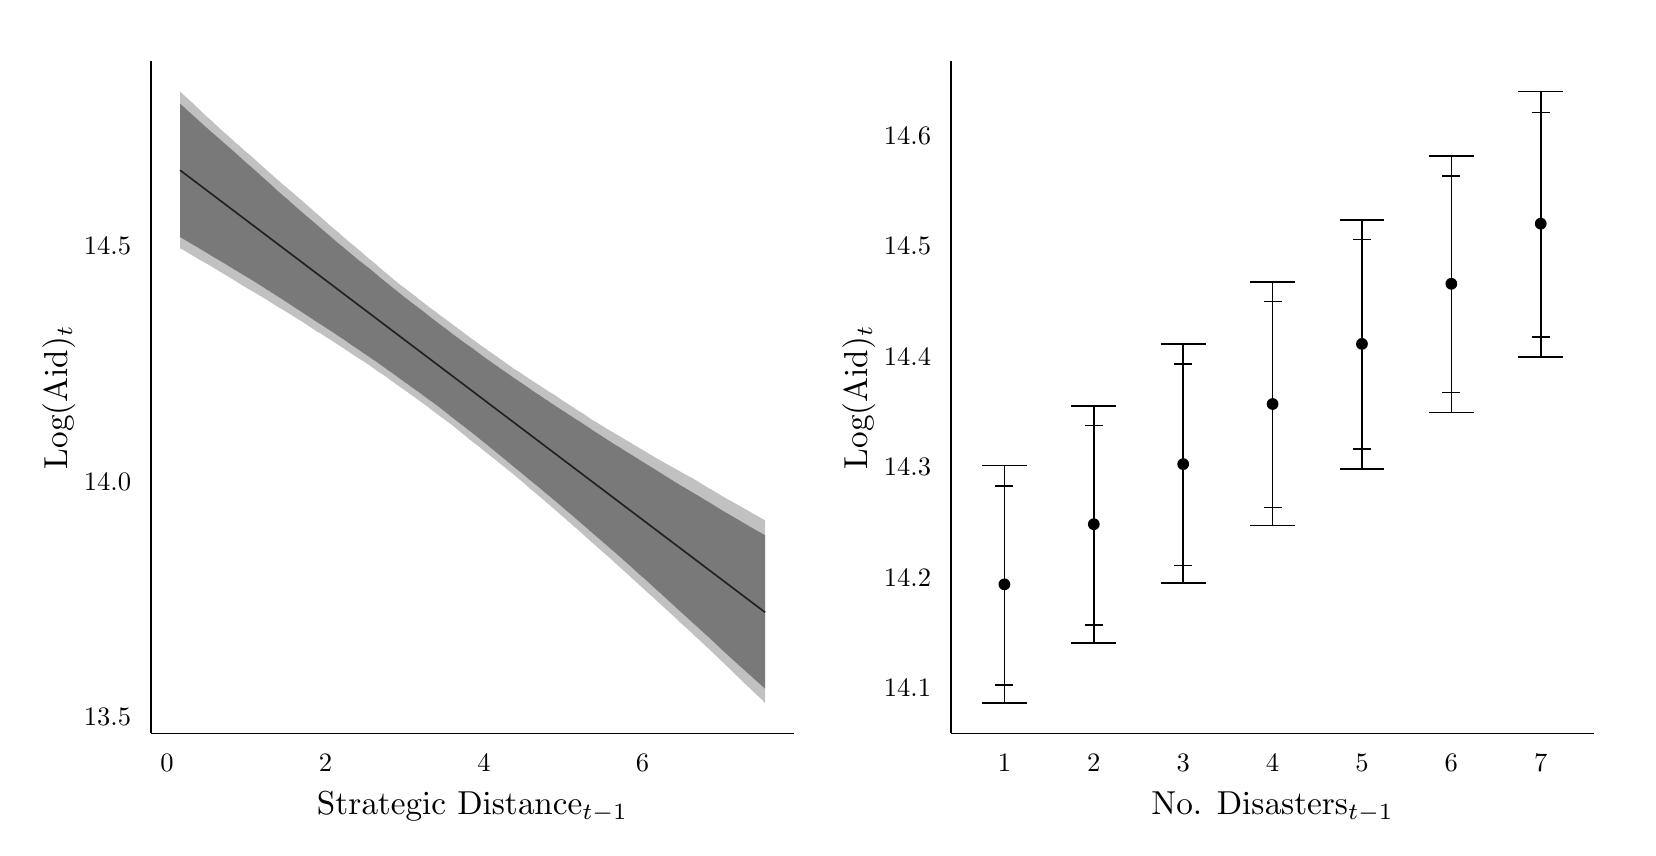
\begin{tikzpicture}[x=1pt,y=1pt]
\definecolor{fillColor}{RGB}{255,255,255}
\path[use as bounding box,fill=fillColor,fill opacity=0.00] (0,0) rectangle (578.16,289.08);
\begin{scope}
\path[clip] (  0.00,  0.00) rectangle (289.08,289.08);
\definecolor{drawColor}{RGB}{255,255,255}
\definecolor{fillColor}{RGB}{255,255,255}

\path[draw=drawColor,line width= 0.6pt,line join=round,line cap=round,fill=fillColor] ( -0.00,  0.00) rectangle (289.08,289.08);
\end{scope}
\begin{scope}
\path[clip] ( 44.49, 34.03) rectangle (277.04,277.03);
\definecolor{fillColor}{RGB}{255,255,255}

\path[fill=fillColor] ( 44.49, 34.03) rectangle (277.04,277.03);
\definecolor{drawColor}{RGB}{0,0,0}

\path[draw=drawColor,line width= 0.6pt,line join=round] ( 55.06,237.59) --
	( 55.34,237.37) --
	( 55.63,237.15) --
	( 55.92,236.94) --
	( 56.20,236.72) --
	( 56.49,236.50) --
	( 56.77,236.29) --
	( 57.06,236.07) --
	( 57.35,235.85) --
	( 57.63,235.64) --
	( 57.92,235.42) --
	( 58.21,235.21) --
	( 58.49,234.99) --
	( 58.78,234.77) --
	( 59.07,234.56) --
	( 59.35,234.34) --
	( 59.64,234.12) --
	( 59.93,233.91) --
	( 60.21,233.69) --
	( 60.50,233.47) --
	( 60.79,233.26) --
	( 61.07,233.04) --
	( 61.36,232.82) --
	( 61.64,232.61) --
	( 61.93,232.39) --
	( 62.22,232.17) --
	( 62.50,231.96) --
	( 62.79,231.74) --
	( 63.08,231.52) --
	( 63.36,231.31) --
	( 63.65,231.09) --
	( 63.94,230.88) --
	( 64.22,230.66) --
	( 64.51,230.44) --
	( 64.80,230.23) --
	( 65.08,230.01) --
	( 65.37,229.79) --
	( 65.65,229.58) --
	( 65.94,229.36) --
	( 66.23,229.14) --
	( 66.51,228.93) --
	( 66.80,228.71) --
	( 67.09,228.49) --
	( 67.37,228.28) --
	( 67.66,228.06) --
	( 67.95,227.84) --
	( 68.23,227.63) --
	( 68.52,227.41) --
	( 68.81,227.19) --
	( 69.09,226.98) --
	( 69.38,226.76) --
	( 69.67,226.55) --
	( 69.95,226.33) --
	( 70.24,226.11) --
	( 70.52,225.90) --
	( 70.81,225.68) --
	( 71.10,225.46) --
	( 71.38,225.25) --
	( 71.67,225.03) --
	( 71.96,224.81) --
	( 72.24,224.60) --
	( 72.53,224.38) --
	( 72.82,224.16) --
	( 73.10,223.95) --
	( 73.39,223.73) --
	( 73.68,223.51) --
	( 73.96,223.30) --
	( 74.25,223.08) --
	( 74.54,222.86) --
	( 74.82,222.65) --
	( 75.11,222.43) --
	( 75.39,222.22) --
	( 75.68,222.00) --
	( 75.97,221.78) --
	( 76.25,221.57) --
	( 76.54,221.35) --
	( 76.83,221.13) --
	( 77.11,220.92) --
	( 77.40,220.70) --
	( 77.69,220.48) --
	( 77.97,220.27) --
	( 78.26,220.05) --
	( 78.55,219.83) --
	( 78.83,219.62) --
	( 79.12,219.40) --
	( 79.41,219.18) --
	( 79.69,218.97) --
	( 79.98,218.75) --
	( 80.26,218.53) --
	( 80.55,218.32) --
	( 80.84,218.10) --
	( 81.12,217.89) --
	( 81.41,217.67) --
	( 81.70,217.45) --
	( 81.98,217.24) --
	( 82.27,217.02) --
	( 82.56,216.80) --
	( 82.84,216.59) --
	( 83.13,216.37) --
	( 83.42,216.15) --
	( 83.70,215.94) --
	( 83.99,215.72) --
	( 84.27,215.50) --
	( 84.56,215.29) --
	( 84.85,215.07) --
	( 85.13,214.85) --
	( 85.42,214.64) --
	( 85.71,214.42) --
	( 85.99,214.20) --
	( 86.28,213.99) --
	( 86.57,213.77) --
	( 86.85,213.56) --
	( 87.14,213.34) --
	( 87.43,213.12) --
	( 87.71,212.91) --
	( 88.00,212.69) --
	( 88.29,212.47) --
	( 88.57,212.26) --
	( 88.86,212.04) --
	( 89.14,211.82) --
	( 89.43,211.61) --
	( 89.72,211.39) --
	( 90.00,211.17) --
	( 90.29,210.96) --
	( 90.58,210.74) --
	( 90.86,210.52) --
	( 91.15,210.31) --
	( 91.44,210.09) --
	( 91.72,209.87) --
	( 92.01,209.66) --
	( 92.30,209.44) --
	( 92.58,209.23) --
	( 92.87,209.01) --
	( 93.16,208.79) --
	( 93.44,208.58) --
	( 93.73,208.36) --
	( 94.01,208.14) --
	( 94.30,207.93) --
	( 94.59,207.71) --
	( 94.87,207.49) --
	( 95.16,207.28) --
	( 95.45,207.06) --
	( 95.73,206.84) --
	( 96.02,206.63) --
	( 96.31,206.41) --
	( 96.59,206.19) --
	( 96.88,205.98) --
	( 97.17,205.76) --
	( 97.45,205.54) --
	( 97.74,205.33) --
	( 98.03,205.11) --
	( 98.31,204.90) --
	( 98.60,204.68) --
	( 98.88,204.46) --
	( 99.17,204.25) --
	( 99.46,204.03) --
	( 99.74,203.81) --
	(100.03,203.60) --
	(100.32,203.38) --
	(100.60,203.16) --
	(100.89,202.95) --
	(101.18,202.73) --
	(101.46,202.51) --
	(101.75,202.30) --
	(102.04,202.08) --
	(102.32,201.86) --
	(102.61,201.65) --
	(102.89,201.43) --
	(103.18,201.21) --
	(103.47,201.00) --
	(103.75,200.78) --
	(104.04,200.57) --
	(104.33,200.35) --
	(104.61,200.13) --
	(104.90,199.92) --
	(105.19,199.70) --
	(105.47,199.48) --
	(105.76,199.27) --
	(106.05,199.05) --
	(106.33,198.83) --
	(106.62,198.62) --
	(106.91,198.40) --
	(107.19,198.18) --
	(107.48,197.97) --
	(107.76,197.75) --
	(108.05,197.53) --
	(108.34,197.32) --
	(108.62,197.10) --
	(108.91,196.88) --
	(109.20,196.67) --
	(109.48,196.45) --
	(109.77,196.24) --
	(110.06,196.02) --
	(110.34,195.80) --
	(110.63,195.59) --
	(110.92,195.37) --
	(111.20,195.15) --
	(111.49,194.94) --
	(111.78,194.72) --
	(112.06,194.50) --
	(112.35,194.29) --
	(112.63,194.07) --
	(112.92,193.85) --
	(113.21,193.64) --
	(113.49,193.42) --
	(113.78,193.20) --
	(114.07,192.99) --
	(114.35,192.77) --
	(114.64,192.55) --
	(114.93,192.34) --
	(115.21,192.12) --
	(115.50,191.91) --
	(115.79,191.69) --
	(116.07,191.47) --
	(116.36,191.26) --
	(116.65,191.04) --
	(116.93,190.82) --
	(117.22,190.61) --
	(117.50,190.39) --
	(117.79,190.17) --
	(118.08,189.96) --
	(118.36,189.74) --
	(118.65,189.52) --
	(118.94,189.31) --
	(119.22,189.09) --
	(119.51,188.87) --
	(119.80,188.66) --
	(120.08,188.44) --
	(120.37,188.22) --
	(120.66,188.01) --
	(120.94,187.79) --
	(121.23,187.58) --
	(121.51,187.36) --
	(121.80,187.14) --
	(122.09,186.93) --
	(122.37,186.71) --
	(122.66,186.49) --
	(122.95,186.28) --
	(123.23,186.06) --
	(123.52,185.84) --
	(123.81,185.63) --
	(124.09,185.41) --
	(124.38,185.19) --
	(124.67,184.98) --
	(124.95,184.76) --
	(125.24,184.54) --
	(125.53,184.33) --
	(125.81,184.11) --
	(126.10,183.89) --
	(126.38,183.68) --
	(126.67,183.46) --
	(126.96,183.25) --
	(127.24,183.03) --
	(127.53,182.81) --
	(127.82,182.60) --
	(128.10,182.38) --
	(128.39,182.16) --
	(128.68,181.95) --
	(128.96,181.73) --
	(129.25,181.51) --
	(129.54,181.30) --
	(129.82,181.08) --
	(130.11,180.86) --
	(130.40,180.65) --
	(130.68,180.43) --
	(130.97,180.21) --
	(131.25,180.00) --
	(131.54,179.78) --
	(131.83,179.56) --
	(132.11,179.35) --
	(132.40,179.13) --
	(132.69,178.92) --
	(132.97,178.70) --
	(133.26,178.48) --
	(133.55,178.27) --
	(133.83,178.05) --
	(134.12,177.83) --
	(134.41,177.62) --
	(134.69,177.40) --
	(134.98,177.18) --
	(135.27,176.97) --
	(135.55,176.75) --
	(135.84,176.53) --
	(136.12,176.32) --
	(136.41,176.10) --
	(136.70,175.88) --
	(136.98,175.67) --
	(137.27,175.45) --
	(137.56,175.23) --
	(137.84,175.02) --
	(138.13,174.80) --
	(138.42,174.59) --
	(138.70,174.37) --
	(138.99,174.15) --
	(139.28,173.94) --
	(139.56,173.72) --
	(139.85,173.50) --
	(140.13,173.29) --
	(140.42,173.07) --
	(140.71,172.85) --
	(140.99,172.64) --
	(141.28,172.42) --
	(141.57,172.20) --
	(141.85,171.99) --
	(142.14,171.77) --
	(142.43,171.55) --
	(142.71,171.34) --
	(143.00,171.12) --
	(143.29,170.90) --
	(143.57,170.69) --
	(143.86,170.47) --
	(144.15,170.26) --
	(144.43,170.04) --
	(144.72,169.82) --
	(145.00,169.61) --
	(145.29,169.39) --
	(145.58,169.17) --
	(145.86,168.96) --
	(146.15,168.74) --
	(146.44,168.52) --
	(146.72,168.31) --
	(147.01,168.09) --
	(147.30,167.87) --
	(147.58,167.66) --
	(147.87,167.44) --
	(148.16,167.22) --
	(148.44,167.01) --
	(148.73,166.79) --
	(149.02,166.57) --
	(149.30,166.36) --
	(149.59,166.14) --
	(149.87,165.93) --
	(150.16,165.71) --
	(150.45,165.49) --
	(150.73,165.28) --
	(151.02,165.06) --
	(151.31,164.84) --
	(151.59,164.63) --
	(151.88,164.41) --
	(152.17,164.19) --
	(152.45,163.98) --
	(152.74,163.76) --
	(153.03,163.54) --
	(153.31,163.33) --
	(153.60,163.11) --
	(153.89,162.89) --
	(154.17,162.68) --
	(154.46,162.46) --
	(154.74,162.24) --
	(155.03,162.03) --
	(155.32,161.81) --
	(155.60,161.60) --
	(155.89,161.38) --
	(156.18,161.16) --
	(156.46,160.95) --
	(156.75,160.73) --
	(157.04,160.51) --
	(157.32,160.30) --
	(157.61,160.08) --
	(157.90,159.86) --
	(158.18,159.65) --
	(158.47,159.43) --
	(158.75,159.21) --
	(159.04,159.00) --
	(159.33,158.78) --
	(159.61,158.56) --
	(159.90,158.35) --
	(160.19,158.13) --
	(160.47,157.91) --
	(160.76,157.70) --
	(161.05,157.48) --
	(161.33,157.27) --
	(161.62,157.05) --
	(161.91,156.83) --
	(162.19,156.62) --
	(162.48,156.40) --
	(162.77,156.18) --
	(163.05,155.97) --
	(163.34,155.75) --
	(163.62,155.53) --
	(163.91,155.32) --
	(164.20,155.10) --
	(164.48,154.88) --
	(164.77,154.67) --
	(165.06,154.45) --
	(165.34,154.23) --
	(165.63,154.02) --
	(165.92,153.80) --
	(166.20,153.58) --
	(166.49,153.37) --
	(166.78,153.15) --
	(167.06,152.94) --
	(167.35,152.72) --
	(167.64,152.50) --
	(167.92,152.29) --
	(168.21,152.07) --
	(168.49,151.85) --
	(168.78,151.64) --
	(169.07,151.42) --
	(169.35,151.20) --
	(169.64,150.99) --
	(169.93,150.77) --
	(170.21,150.55) --
	(170.50,150.34) --
	(170.79,150.12) --
	(171.07,149.90) --
	(171.36,149.69) --
	(171.65,149.47) --
	(171.93,149.25) --
	(172.22,149.04) --
	(172.51,148.82) --
	(172.79,148.61) --
	(173.08,148.39) --
	(173.36,148.17) --
	(173.65,147.96) --
	(173.94,147.74) --
	(174.22,147.52) --
	(174.51,147.31) --
	(174.80,147.09) --
	(175.08,146.87) --
	(175.37,146.66) --
	(175.66,146.44) --
	(175.94,146.22) --
	(176.23,146.01) --
	(176.52,145.79) --
	(176.80,145.57) --
	(177.09,145.36) --
	(177.37,145.14) --
	(177.66,144.92) --
	(177.95,144.71) --
	(178.23,144.49) --
	(178.52,144.28) --
	(178.81,144.06) --
	(179.09,143.84) --
	(179.38,143.63) --
	(179.67,143.41) --
	(179.95,143.19) --
	(180.24,142.98) --
	(180.53,142.76) --
	(180.81,142.54) --
	(181.10,142.33) --
	(181.39,142.11) --
	(181.67,141.89) --
	(181.96,141.68) --
	(182.24,141.46) --
	(182.53,141.24) --
	(182.82,141.03) --
	(183.10,140.81) --
	(183.39,140.59) --
	(183.68,140.38) --
	(183.96,140.16) --
	(184.25,139.95) --
	(184.54,139.73) --
	(184.82,139.51) --
	(185.11,139.30) --
	(185.40,139.08) --
	(185.68,138.86) --
	(185.97,138.65) --
	(186.26,138.43) --
	(186.54,138.21) --
	(186.83,138.00) --
	(187.11,137.78) --
	(187.40,137.56) --
	(187.69,137.35) --
	(187.97,137.13) --
	(188.26,136.91) --
	(188.55,136.70) --
	(188.83,136.48) --
	(189.12,136.26) --
	(189.41,136.05) --
	(189.69,135.83) --
	(189.98,135.62) --
	(190.27,135.40) --
	(190.55,135.18) --
	(190.84,134.97) --
	(191.13,134.75) --
	(191.41,134.53) --
	(191.70,134.32) --
	(191.98,134.10) --
	(192.27,133.88) --
	(192.56,133.67) --
	(192.84,133.45) --
	(193.13,133.23) --
	(193.42,133.02) --
	(193.70,132.80) --
	(193.99,132.58) --
	(194.28,132.37) --
	(194.56,132.15) --
	(194.85,131.93) --
	(195.14,131.72) --
	(195.42,131.50) --
	(195.71,131.29) --
	(195.99,131.07) --
	(196.28,130.85) --
	(196.57,130.64) --
	(196.85,130.42) --
	(197.14,130.20) --
	(197.43,129.99) --
	(197.71,129.77) --
	(198.00,129.55) --
	(198.29,129.34) --
	(198.57,129.12) --
	(198.86,128.90) --
	(199.15,128.69) --
	(199.43,128.47) --
	(199.72,128.25) --
	(200.01,128.04) --
	(200.29,127.82) --
	(200.58,127.60) --
	(200.86,127.39) --
	(201.15,127.17) --
	(201.44,126.96) --
	(201.72,126.74) --
	(202.01,126.52) --
	(202.30,126.31) --
	(202.58,126.09) --
	(202.87,125.87) --
	(203.16,125.66) --
	(203.44,125.44) --
	(203.73,125.22) --
	(204.02,125.01) --
	(204.30,124.79) --
	(204.59,124.57) --
	(204.88,124.36) --
	(205.16,124.14) --
	(205.45,123.92) --
	(205.73,123.71) --
	(206.02,123.49) --
	(206.31,123.28) --
	(206.59,123.06) --
	(206.88,122.84) --
	(207.17,122.63) --
	(207.45,122.41) --
	(207.74,122.19) --
	(208.03,121.98) --
	(208.31,121.76) --
	(208.60,121.54) --
	(208.89,121.33) --
	(209.17,121.11) --
	(209.46,120.89) --
	(209.75,120.68) --
	(210.03,120.46) --
	(210.32,120.24) --
	(210.60,120.03) --
	(210.89,119.81) --
	(211.18,119.59) --
	(211.46,119.38) --
	(211.75,119.16) --
	(212.04,118.95) --
	(212.32,118.73) --
	(212.61,118.51) --
	(212.90,118.30) --
	(213.18,118.08) --
	(213.47,117.86) --
	(213.76,117.65) --
	(214.04,117.43) --
	(214.33,117.21) --
	(214.62,117.00) --
	(214.90,116.78) --
	(215.19,116.56) --
	(215.47,116.35) --
	(215.76,116.13) --
	(216.05,115.91) --
	(216.33,115.70) --
	(216.62,115.48) --
	(216.91,115.26) --
	(217.19,115.05) --
	(217.48,114.83) --
	(217.77,114.62) --
	(218.05,114.40) --
	(218.34,114.18) --
	(218.63,113.97) --
	(218.91,113.75) --
	(219.20,113.53) --
	(219.48,113.32) --
	(219.77,113.10) --
	(220.06,112.88) --
	(220.34,112.67) --
	(220.63,112.45) --
	(220.92,112.23) --
	(221.20,112.02) --
	(221.49,111.80) --
	(221.78,111.58) --
	(222.06,111.37) --
	(222.35,111.15) --
	(222.64,110.93) --
	(222.92,110.72) --
	(223.21,110.50) --
	(223.50,110.29) --
	(223.78,110.07) --
	(224.07,109.85) --
	(224.35,109.64) --
	(224.64,109.42) --
	(224.93,109.20) --
	(225.21,108.99) --
	(225.50,108.77) --
	(225.79,108.55) --
	(226.07,108.34) --
	(226.36,108.12) --
	(226.65,107.90) --
	(226.93,107.69) --
	(227.22,107.47) --
	(227.51,107.25) --
	(227.79,107.04) --
	(228.08,106.82) --
	(228.37,106.60) --
	(228.65,106.39) --
	(228.94,106.17) --
	(229.22,105.96) --
	(229.51,105.74) --
	(229.80,105.52) --
	(230.08,105.31) --
	(230.37,105.09) --
	(230.66,104.87) --
	(230.94,104.66) --
	(231.23,104.44) --
	(231.52,104.22) --
	(231.80,104.01) --
	(232.09,103.79) --
	(232.38,103.57) --
	(232.66,103.36) --
	(232.95,103.14) --
	(233.24,102.92) --
	(233.52,102.71) --
	(233.81,102.49) --
	(234.09,102.27) --
	(234.38,102.06) --
	(234.67,101.84) --
	(234.95,101.63) --
	(235.24,101.41) --
	(235.53,101.19) --
	(235.81,100.98) --
	(236.10,100.76) --
	(236.39,100.54) --
	(236.67,100.33) --
	(236.96,100.11) --
	(237.25, 99.89) --
	(237.53, 99.68) --
	(237.82, 99.46) --
	(238.10, 99.24) --
	(238.39, 99.03) --
	(238.68, 98.81) --
	(238.96, 98.59) --
	(239.25, 98.38) --
	(239.54, 98.16) --
	(239.82, 97.94) --
	(240.11, 97.73) --
	(240.40, 97.51) --
	(240.68, 97.30) --
	(240.97, 97.08) --
	(241.26, 96.86) --
	(241.54, 96.65) --
	(241.83, 96.43) --
	(242.12, 96.21) --
	(242.40, 96.00) --
	(242.69, 95.78) --
	(242.97, 95.56) --
	(243.26, 95.35) --
	(243.55, 95.13) --
	(243.83, 94.91) --
	(244.12, 94.70) --
	(244.41, 94.48) --
	(244.69, 94.26) --
	(244.98, 94.05) --
	(245.27, 93.83) --
	(245.55, 93.61) --
	(245.84, 93.40) --
	(246.13, 93.18) --
	(246.41, 92.97) --
	(246.70, 92.75) --
	(246.99, 92.53) --
	(247.27, 92.32) --
	(247.56, 92.10) --
	(247.84, 91.88) --
	(248.13, 91.67) --
	(248.42, 91.45) --
	(248.70, 91.23) --
	(248.99, 91.02) --
	(249.28, 90.80) --
	(249.56, 90.58) --
	(249.85, 90.37) --
	(250.14, 90.15) --
	(250.42, 89.93) --
	(250.71, 89.72) --
	(251.00, 89.50) --
	(251.28, 89.28) --
	(251.57, 89.07) --
	(251.86, 88.85) --
	(252.14, 88.64) --
	(252.43, 88.42) --
	(252.71, 88.20) --
	(253.00, 87.99) --
	(253.29, 87.77) --
	(253.57, 87.55) --
	(253.86, 87.34) --
	(254.15, 87.12) --
	(254.43, 86.90) --
	(254.72, 86.69) --
	(255.01, 86.47) --
	(255.29, 86.25) --
	(255.58, 86.04) --
	(255.87, 85.82) --
	(256.15, 85.60) --
	(256.44, 85.39) --
	(256.72, 85.17) --
	(257.01, 84.95) --
	(257.30, 84.74) --
	(257.58, 84.52) --
	(257.87, 84.31) --
	(258.16, 84.09) --
	(258.44, 83.87) --
	(258.73, 83.66) --
	(259.02, 83.44) --
	(259.30, 83.22) --
	(259.59, 83.01) --
	(259.88, 82.79) --
	(260.16, 82.57) --
	(260.45, 82.36) --
	(260.74, 82.14) --
	(261.02, 81.92) --
	(261.31, 81.71) --
	(261.59, 81.49) --
	(261.88, 81.27) --
	(262.17, 81.06) --
	(262.45, 80.84) --
	(262.74, 80.62) --
	(263.03, 80.41) --
	(263.31, 80.19) --
	(263.60, 79.98) --
	(263.89, 79.76) --
	(264.17, 79.54) --
	(264.46, 79.33) --
	(264.75, 79.11) --
	(265.03, 78.89) --
	(265.32, 78.68) --
	(265.61, 78.46) --
	(265.89, 78.24) --
	(266.18, 78.03) --
	(266.46, 77.81);
\definecolor{fillColor}{RGB}{51,51,51}

\path[fill=fillColor,fill opacity=0.30] ( 55.06,265.99) --
	( 55.34,265.72) --
	( 55.63,265.47) --
	( 55.92,265.19) --
	( 56.20,264.92) --
	( 56.49,264.67) --
	( 56.77,264.41) --
	( 57.06,264.16) --
	( 57.35,263.90) --
	( 57.63,263.65) --
	( 57.92,263.39) --
	( 58.21,263.10) --
	( 58.49,262.84) --
	( 58.78,262.57) --
	( 59.07,262.32) --
	( 59.35,262.07) --
	( 59.64,261.80) --
	( 59.93,261.57) --
	( 60.21,261.30) --
	( 60.50,260.98) --
	( 60.79,260.70) --
	( 61.07,260.42) --
	( 61.36,260.15) --
	( 61.64,259.89) --
	( 61.93,259.63) --
	( 62.22,259.36) --
	( 62.50,259.06) --
	( 62.79,258.76) --
	( 63.08,258.49) --
	( 63.36,258.19) --
	( 63.65,257.91) --
	( 63.94,257.66) --
	( 64.22,257.41) --
	( 64.51,257.15) --
	( 64.80,256.86) --
	( 65.08,256.62) --
	( 65.37,256.39) --
	( 65.65,256.13) --
	( 65.94,255.89) --
	( 66.23,255.65) --
	( 66.51,255.37) --
	( 66.80,255.10) --
	( 67.09,254.83) --
	( 67.37,254.56) --
	( 67.66,254.28) --
	( 67.95,254.02) --
	( 68.23,253.75) --
	( 68.52,253.50) --
	( 68.81,253.24) --
	( 69.09,252.96) --
	( 69.38,252.70) --
	( 69.67,252.42) --
	( 69.95,252.15) --
	( 70.24,251.88) --
	( 70.52,251.62) --
	( 70.81,251.36) --
	( 71.10,251.12) --
	( 71.38,250.89) --
	( 71.67,250.65) --
	( 71.96,250.40) --
	( 72.24,250.15) --
	( 72.53,249.91) --
	( 72.82,249.63) --
	( 73.10,249.37) --
	( 73.39,249.14) --
	( 73.68,248.89) --
	( 73.96,248.64) --
	( 74.25,248.39) --
	( 74.54,248.12) --
	( 74.82,247.84) --
	( 75.11,247.56) --
	( 75.39,247.29) --
	( 75.68,247.06) --
	( 75.97,246.83) --
	( 76.25,246.59) --
	( 76.54,246.34) --
	( 76.83,246.09) --
	( 77.11,245.84) --
	( 77.40,245.57) --
	( 77.69,245.29) --
	( 77.97,245.01) --
	( 78.26,244.76) --
	( 78.55,244.50) --
	( 78.83,244.26) --
	( 79.12,244.03) --
	( 79.41,243.81) --
	( 79.69,243.59) --
	( 79.98,243.37) --
	( 80.26,243.10) --
	( 80.55,242.86) --
	( 80.84,242.58) --
	( 81.12,242.33) --
	( 81.41,242.08) --
	( 81.70,241.81) --
	( 81.98,241.57) --
	( 82.27,241.28) --
	( 82.56,241.03) --
	( 82.84,240.75) --
	( 83.13,240.51) --
	( 83.42,240.26) --
	( 83.70,240.02) --
	( 83.99,239.75) --
	( 84.27,239.47) --
	( 84.56,239.23) --
	( 84.85,238.97) --
	( 85.13,238.72) --
	( 85.42,238.48) --
	( 85.71,238.21) --
	( 85.99,237.97) --
	( 86.28,237.69) --
	( 86.57,237.42) --
	( 86.85,237.19) --
	( 87.14,236.95) --
	( 87.43,236.67) --
	( 87.71,236.42) --
	( 88.00,236.17) --
	( 88.29,235.93) --
	( 88.57,235.68) --
	( 88.86,235.40) --
	( 89.14,235.17) --
	( 89.43,234.92) --
	( 89.72,234.66) --
	( 90.00,234.37) --
	( 90.29,234.12) --
	( 90.58,233.88) --
	( 90.86,233.62) --
	( 91.15,233.35) --
	( 91.44,233.13) --
	( 91.72,232.86) --
	( 92.01,232.57) --
	( 92.30,232.34) --
	( 92.58,232.10) --
	( 92.87,231.89) --
	( 93.16,231.67) --
	( 93.44,231.41) --
	( 93.73,231.17) --
	( 94.01,230.94) --
	( 94.30,230.71) --
	( 94.59,230.47) --
	( 94.87,230.23) --
	( 95.16,230.00) --
	( 95.45,229.75) --
	( 95.73,229.49) --
	( 96.02,229.26) --
	( 96.31,229.03) --
	( 96.59,228.74) --
	( 96.88,228.47) --
	( 97.17,228.23) --
	( 97.45,228.01) --
	( 97.74,227.78) --
	( 98.03,227.52) --
	( 98.31,227.27) --
	( 98.60,227.00) --
	( 98.88,226.77) --
	( 99.17,226.55) --
	( 99.46,226.24) --
	( 99.74,226.00) --
	(100.03,225.76) --
	(100.32,225.51) --
	(100.60,225.28) --
	(100.89,225.00) --
	(101.18,224.75) --
	(101.46,224.50) --
	(101.75,224.25) --
	(102.04,224.00) --
	(102.32,223.74) --
	(102.61,223.50) --
	(102.89,223.26) --
	(103.18,223.01) --
	(103.47,222.75) --
	(103.75,222.50) --
	(104.04,222.24) --
	(104.33,222.01) --
	(104.61,221.76) --
	(104.90,221.51) --
	(105.19,221.25) --
	(105.47,221.00) --
	(105.76,220.75) --
	(106.05,220.49) --
	(106.33,220.25) --
	(106.62,219.99) --
	(106.91,219.73) --
	(107.19,219.50) --
	(107.48,219.21) --
	(107.76,218.94) --
	(108.05,218.68) --
	(108.34,218.42) --
	(108.62,218.17) --
	(108.91,217.92) --
	(109.20,217.66) --
	(109.48,217.41) --
	(109.77,217.16) --
	(110.06,216.92) --
	(110.34,216.69) --
	(110.63,216.47) --
	(110.92,216.24) --
	(111.20,215.99) --
	(111.49,215.76) --
	(111.78,215.54) --
	(112.06,215.31) --
	(112.35,215.04) --
	(112.63,214.76) --
	(112.92,214.48) --
	(113.21,214.25) --
	(113.49,213.98) --
	(113.78,213.72) --
	(114.07,213.48) --
	(114.35,213.24) --
	(114.64,213.01) --
	(114.93,212.77) --
	(115.21,212.49) --
	(115.50,212.25) --
	(115.79,211.99) --
	(116.07,211.76) --
	(116.36,211.49) --
	(116.65,211.27) --
	(116.93,211.08) --
	(117.22,210.81) --
	(117.50,210.57) --
	(117.79,210.34) --
	(118.08,210.11) --
	(118.36,209.88) --
	(118.65,209.64) --
	(118.94,209.39) --
	(119.22,209.15) --
	(119.51,208.90) --
	(119.80,208.67) --
	(120.08,208.45) --
	(120.37,208.22) --
	(120.66,207.97) --
	(120.94,207.67) --
	(121.23,207.42) --
	(121.51,207.17) --
	(121.80,206.91) --
	(122.09,206.69) --
	(122.37,206.43) --
	(122.66,206.17) --
	(122.95,205.91) --
	(123.23,205.66) --
	(123.52,205.42) --
	(123.81,205.26) --
	(124.09,205.00) --
	(124.38,204.74) --
	(124.67,204.52) --
	(124.95,204.31) --
	(125.24,204.08) --
	(125.53,203.83) --
	(125.81,203.59) --
	(126.10,203.40) --
	(126.38,203.16) --
	(126.67,202.87) --
	(126.96,202.59) --
	(127.24,202.33) --
	(127.53,202.10) --
	(127.82,201.83) --
	(128.10,201.58) --
	(128.39,201.32) --
	(128.68,201.07) --
	(128.96,200.86) --
	(129.25,200.66) --
	(129.54,200.38) --
	(129.82,200.15) --
	(130.11,199.89) --
	(130.40,199.67) --
	(130.68,199.42) --
	(130.97,199.17) --
	(131.25,198.92) --
	(131.54,198.68) --
	(131.83,198.44) --
	(132.11,198.21) --
	(132.40,197.97) --
	(132.69,197.73) --
	(132.97,197.48) --
	(133.26,197.23) --
	(133.55,197.03) --
	(133.83,196.77) --
	(134.12,196.55) --
	(134.41,196.35) --
	(134.69,196.12) --
	(134.98,195.89) --
	(135.27,195.67) --
	(135.55,195.49) --
	(135.84,195.28) --
	(136.12,195.09) --
	(136.41,194.86) --
	(136.70,194.64) --
	(136.98,194.41) --
	(137.27,194.19) --
	(137.56,193.98) --
	(137.84,193.73) --
	(138.13,193.51) --
	(138.42,193.27) --
	(138.70,193.09) --
	(138.99,192.88) --
	(139.28,192.66) --
	(139.56,192.44) --
	(139.85,192.25) --
	(140.13,192.04) --
	(140.42,191.80) --
	(140.71,191.56) --
	(140.99,191.31) --
	(141.28,191.06) --
	(141.57,190.82) --
	(141.85,190.61) --
	(142.14,190.39) --
	(142.43,190.15) --
	(142.71,189.93) --
	(143.00,189.74) --
	(143.29,189.49) --
	(143.57,189.27) --
	(143.86,189.05) --
	(144.15,188.87) --
	(144.43,188.64) --
	(144.72,188.42) --
	(145.00,188.22) --
	(145.29,187.96) --
	(145.58,187.75) --
	(145.86,187.55) --
	(146.15,187.33) --
	(146.44,187.12) --
	(146.72,186.92) --
	(147.01,186.69) --
	(147.30,186.48) --
	(147.58,186.27) --
	(147.87,186.05) --
	(148.16,185.84) --
	(148.44,185.63) --
	(148.73,185.42) --
	(149.02,185.18) --
	(149.30,184.97) --
	(149.59,184.76) --
	(149.87,184.57) --
	(150.16,184.36) --
	(150.45,184.14) --
	(150.73,183.96) --
	(151.02,183.72) --
	(151.31,183.52) --
	(151.59,183.31) --
	(151.88,183.10) --
	(152.17,182.87) --
	(152.45,182.66) --
	(152.74,182.44) --
	(153.03,182.23) --
	(153.31,182.00) --
	(153.60,181.79) --
	(153.89,181.59) --
	(154.17,181.38) --
	(154.46,181.18) --
	(154.74,180.96) --
	(155.03,180.75) --
	(155.32,180.53) --
	(155.60,180.31) --
	(155.89,180.11) --
	(156.18,179.91) --
	(156.46,179.70) --
	(156.75,179.47) --
	(157.04,179.23) --
	(157.32,179.02) --
	(157.61,178.82) --
	(157.90,178.58) --
	(158.18,178.35) --
	(158.47,178.11) --
	(158.75,177.88) --
	(159.04,177.69) --
	(159.33,177.49) --
	(159.61,177.32) --
	(159.90,177.08) --
	(160.19,176.85) --
	(160.47,176.66) --
	(160.76,176.44) --
	(161.05,176.28) --
	(161.33,176.07) --
	(161.62,175.86) --
	(161.91,175.65) --
	(162.19,175.43) --
	(162.48,175.19) --
	(162.77,174.98) --
	(163.05,174.76) --
	(163.34,174.58) --
	(163.62,174.35) --
	(163.91,174.16) --
	(164.20,173.95) --
	(164.48,173.75) --
	(164.77,173.57) --
	(165.06,173.41) --
	(165.34,173.20) --
	(165.63,172.99) --
	(165.92,172.79) --
	(166.20,172.58) --
	(166.49,172.35) --
	(166.78,172.15) --
	(167.06,171.95) --
	(167.35,171.76) --
	(167.64,171.54) --
	(167.92,171.34) --
	(168.21,171.15) --
	(168.49,170.96) --
	(168.78,170.73) --
	(169.07,170.55) --
	(169.35,170.37) --
	(169.64,170.18) --
	(169.93,169.97) --
	(170.21,169.74) --
	(170.50,169.51) --
	(170.79,169.32) --
	(171.07,169.12) --
	(171.36,168.94) --
	(171.65,168.74) --
	(171.93,168.52) --
	(172.22,168.32) --
	(172.51,168.11) --
	(172.79,167.91) --
	(173.08,167.70) --
	(173.36,167.51) --
	(173.65,167.31) --
	(173.94,167.10) --
	(174.22,166.89) --
	(174.51,166.70) --
	(174.80,166.51) --
	(175.08,166.27) --
	(175.37,166.06) --
	(175.66,165.86) --
	(175.94,165.67) --
	(176.23,165.51) --
	(176.52,165.34) --
	(176.80,165.17) --
	(177.09,165.00) --
	(177.37,164.81) --
	(177.66,164.63) --
	(177.95,164.44) --
	(178.23,164.25) --
	(178.52,164.04) --
	(178.81,163.84) --
	(179.09,163.63) --
	(179.38,163.43) --
	(179.67,163.26) --
	(179.95,163.07) --
	(180.24,162.87) --
	(180.53,162.71) --
	(180.81,162.50) --
	(181.10,162.31) --
	(181.39,162.11) --
	(181.67,161.92) --
	(181.96,161.72) --
	(182.24,161.52) --
	(182.53,161.33) --
	(182.82,161.16) --
	(183.10,161.00) --
	(183.39,160.81) --
	(183.68,160.61) --
	(183.96,160.42) --
	(184.25,160.26) --
	(184.54,160.09) --
	(184.82,159.89) --
	(185.11,159.71) --
	(185.40,159.51) --
	(185.68,159.28) --
	(185.97,159.09) --
	(186.26,158.90) --
	(186.54,158.76) --
	(186.83,158.56) --
	(187.11,158.39) --
	(187.40,158.20) --
	(187.69,158.02) --
	(187.97,157.82) --
	(188.26,157.63) --
	(188.55,157.45) --
	(188.83,157.28) --
	(189.12,157.14) --
	(189.41,156.94) --
	(189.69,156.77) --
	(189.98,156.61) --
	(190.27,156.44) --
	(190.55,156.24) --
	(190.84,156.04) --
	(191.13,155.84) --
	(191.41,155.66) --
	(191.70,155.46) --
	(191.98,155.24) --
	(192.27,155.04) --
	(192.56,154.86) --
	(192.84,154.67) --
	(193.13,154.43) --
	(193.42,154.26) --
	(193.70,154.07) --
	(193.99,153.91) --
	(194.28,153.71) --
	(194.56,153.55) --
	(194.85,153.38) --
	(195.14,153.18) --
	(195.42,153.00) --
	(195.71,152.79) --
	(195.99,152.61) --
	(196.28,152.46) --
	(196.57,152.27) --
	(196.85,152.09) --
	(197.14,151.89) --
	(197.43,151.70) --
	(197.71,151.50) --
	(198.00,151.29) --
	(198.29,151.09) --
	(198.57,150.90) --
	(198.86,150.72) --
	(199.15,150.54) --
	(199.43,150.40) --
	(199.72,150.24) --
	(200.01,150.03) --
	(200.29,149.89) --
	(200.58,149.70) --
	(200.86,149.54) --
	(201.15,149.32) --
	(201.44,149.12) --
	(201.72,148.93) --
	(202.01,148.72) --
	(202.30,148.50) --
	(202.58,148.32) --
	(202.87,148.13) --
	(203.16,147.95) --
	(203.44,147.74) --
	(203.73,147.56) --
	(204.02,147.35) --
	(204.30,147.15) --
	(204.59,147.00) --
	(204.88,146.86) --
	(205.16,146.69) --
	(205.45,146.52) --
	(205.73,146.35) --
	(206.02,146.17) --
	(206.31,146.01) --
	(206.59,145.84) --
	(206.88,145.64) --
	(207.17,145.48) --
	(207.45,145.32) --
	(207.74,145.15) --
	(208.03,144.98) --
	(208.31,144.76) --
	(208.60,144.57) --
	(208.89,144.41) --
	(209.17,144.22) --
	(209.46,144.03) --
	(209.75,143.87) --
	(210.03,143.68) --
	(210.32,143.55) --
	(210.60,143.36) --
	(210.89,143.18) --
	(211.18,143.02) --
	(211.46,142.88) --
	(211.75,142.71) --
	(212.04,142.53) --
	(212.32,142.35) --
	(212.61,142.18) --
	(212.90,142.01) --
	(213.18,141.86) --
	(213.47,141.69) --
	(213.76,141.54) --
	(214.04,141.38) --
	(214.33,141.21) --
	(214.62,141.02) --
	(214.90,140.83) --
	(215.19,140.67) --
	(215.47,140.51) --
	(215.76,140.31) --
	(216.05,140.13) --
	(216.33,139.97) --
	(216.62,139.83) --
	(216.91,139.68) --
	(217.19,139.50) --
	(217.48,139.33) --
	(217.77,139.15) --
	(218.05,138.98) --
	(218.34,138.81) --
	(218.63,138.63) --
	(218.91,138.44) --
	(219.20,138.30) --
	(219.48,138.13) --
	(219.77,137.97) --
	(220.06,137.80) --
	(220.34,137.63) --
	(220.63,137.45) --
	(220.92,137.26) --
	(221.20,137.10) --
	(221.49,136.94) --
	(221.78,136.77) --
	(222.06,136.60) --
	(222.35,136.44) --
	(222.64,136.26) --
	(222.92,136.08) --
	(223.21,135.91) --
	(223.50,135.74) --
	(223.78,135.55) --
	(224.07,135.39) --
	(224.35,135.23) --
	(224.64,135.05) --
	(224.93,134.88) --
	(225.21,134.70) --
	(225.50,134.54) --
	(225.79,134.37) --
	(226.07,134.20) --
	(226.36,134.03) --
	(226.65,133.83) --
	(226.93,133.63) --
	(227.22,133.47) --
	(227.51,133.32) --
	(227.79,133.17) --
	(228.08,133.01) --
	(228.37,132.88) --
	(228.65,132.72) --
	(228.94,132.55) --
	(229.22,132.37) --
	(229.51,132.18) --
	(229.80,132.02) --
	(230.08,131.86) --
	(230.37,131.70) --
	(230.66,131.54) --
	(230.94,131.38) --
	(231.23,131.23) --
	(231.52,131.09) --
	(231.80,130.91) --
	(232.09,130.76) --
	(232.38,130.60) --
	(232.66,130.45) --
	(232.95,130.27) --
	(233.24,130.10) --
	(233.52,129.97) --
	(233.81,129.81) --
	(234.09,129.64) --
	(234.38,129.48) --
	(234.67,129.31) --
	(234.95,129.16) --
	(235.24,129.02) --
	(235.53,128.87) --
	(235.81,128.67) --
	(236.10,128.50) --
	(236.39,128.37) --
	(236.67,128.19) --
	(236.96,127.99) --
	(237.25,127.82) --
	(237.53,127.66) --
	(237.82,127.51) --
	(238.10,127.38) --
	(238.39,127.24) --
	(238.68,127.07) --
	(238.96,126.90) --
	(239.25,126.75) --
	(239.54,126.63) --
	(239.82,126.49) --
	(240.11,126.35) --
	(240.40,126.20) --
	(240.68,126.02) --
	(240.97,125.83) --
	(241.26,125.68) --
	(241.54,125.52) --
	(241.83,125.33) --
	(242.12,125.13) --
	(242.40,124.96) --
	(242.69,124.79) --
	(242.97,124.61) --
	(243.26,124.43) --
	(243.55,124.27) --
	(243.83,124.06) --
	(244.12,123.86) --
	(244.41,123.67) --
	(244.69,123.51) --
	(244.98,123.35) --
	(245.27,123.19) --
	(245.55,123.00) --
	(245.84,122.84) --
	(246.13,122.69) --
	(246.41,122.53) --
	(246.70,122.38) --
	(246.99,122.22) --
	(247.27,122.06) --
	(247.56,121.87) --
	(247.84,121.74) --
	(248.13,121.55) --
	(248.42,121.37) --
	(248.70,121.18) --
	(248.99,120.99) --
	(249.28,120.84) --
	(249.56,120.67) --
	(249.85,120.48) --
	(250.14,120.31) --
	(250.42,120.13) --
	(250.71,119.98) --
	(251.00,119.82) --
	(251.28,119.65) --
	(251.57,119.48) --
	(251.86,119.32) --
	(252.14,119.15) --
	(252.43,118.98) --
	(252.71,118.79) --
	(253.00,118.65) --
	(253.29,118.48) --
	(253.57,118.32) --
	(253.86,118.18) --
	(254.15,118.05) --
	(254.43,117.91) --
	(254.72,117.75) --
	(255.01,117.57) --
	(255.29,117.41) --
	(255.58,117.24) --
	(255.87,117.07) --
	(256.15,116.90) --
	(256.44,116.73) --
	(256.72,116.58) --
	(257.01,116.41) --
	(257.30,116.27) --
	(257.58,116.11) --
	(257.87,115.93) --
	(258.16,115.76) --
	(258.44,115.58) --
	(258.73,115.41) --
	(259.02,115.28) --
	(259.30,115.14) --
	(259.59,114.97) --
	(259.88,114.80) --
	(260.16,114.63) --
	(260.45,114.46) --
	(260.74,114.29) --
	(261.02,114.14) --
	(261.31,113.99) --
	(261.59,113.81) --
	(261.88,113.61) --
	(262.17,113.43) --
	(262.45,113.27) --
	(262.74,113.13) --
	(263.03,112.99) --
	(263.31,112.82) --
	(263.60,112.65) --
	(263.89,112.51) --
	(264.17,112.37) --
	(264.46,112.18) --
	(264.75,112.01) --
	(265.03,111.82) --
	(265.32,111.67) --
	(265.61,111.53) --
	(265.89,111.39) --
	(266.18,111.24) --
	(266.46,111.07) --
	(266.46, 45.08) --
	(266.18, 45.37) --
	(265.89, 45.67) --
	(265.61, 45.98) --
	(265.32, 46.25) --
	(265.03, 46.53) --
	(264.75, 46.82) --
	(264.46, 47.06) --
	(264.17, 47.33) --
	(263.89, 47.59) --
	(263.60, 47.86) --
	(263.31, 48.11) --
	(263.03, 48.36) --
	(262.74, 48.65) --
	(262.45, 48.93) --
	(262.17, 49.21) --
	(261.88, 49.47) --
	(261.59, 49.75) --
	(261.31, 50.05) --
	(261.02, 50.34) --
	(260.74, 50.60) --
	(260.45, 50.85) --
	(260.16, 51.13) --
	(259.88, 51.38) --
	(259.59, 51.67) --
	(259.30, 51.91) --
	(259.02, 52.18) --
	(258.73, 52.45) --
	(258.44, 52.72) --
	(258.16, 53.00) --
	(257.87, 53.28) --
	(257.58, 53.56) --
	(257.30, 53.86) --
	(257.01, 54.17) --
	(256.72, 54.43) --
	(256.44, 54.68) --
	(256.15, 54.96) --
	(255.87, 55.24) --
	(255.58, 55.54) --
	(255.29, 55.84) --
	(255.01, 56.09) --
	(254.72, 56.38) --
	(254.43, 56.64) --
	(254.15, 56.91) --
	(253.86, 57.19) --
	(253.57, 57.49) --
	(253.29, 57.78) --
	(253.00, 58.04) --
	(252.71, 58.32) --
	(252.43, 58.58) --
	(252.14, 58.84) --
	(251.86, 59.11) --
	(251.57, 59.39) --
	(251.28, 59.66) --
	(251.00, 59.94) --
	(250.71, 60.22) --
	(250.42, 60.49) --
	(250.14, 60.76) --
	(249.85, 61.04) --
	(249.56, 61.32) --
	(249.28, 61.60) --
	(248.99, 61.88) --
	(248.70, 62.16) --
	(248.42, 62.42) --
	(248.13, 62.70) --
	(247.84, 62.98) --
	(247.56, 63.27) --
	(247.27, 63.55) --
	(246.99, 63.82) --
	(246.70, 64.07) --
	(246.41, 64.36) --
	(246.13, 64.64) --
	(245.84, 64.89) --
	(245.55, 65.10) --
	(245.27, 65.37) --
	(244.98, 65.64) --
	(244.69, 65.92) --
	(244.41, 66.21) --
	(244.12, 66.49) --
	(243.83, 66.74) --
	(243.55, 66.99) --
	(243.26, 67.26) --
	(242.97, 67.54) --
	(242.69, 67.82) --
	(242.40, 68.10) --
	(242.12, 68.36) --
	(241.83, 68.60) --
	(241.54, 68.86) --
	(241.26, 69.12) --
	(240.97, 69.40) --
	(240.68, 69.69) --
	(240.40, 69.97) --
	(240.11, 70.23) --
	(239.82, 70.50) --
	(239.54, 70.76) --
	(239.25, 71.02) --
	(238.96, 71.29) --
	(238.68, 71.58) --
	(238.39, 71.84) --
	(238.10, 72.06) --
	(237.82, 72.31) --
	(237.53, 72.56) --
	(237.25, 72.79) --
	(236.96, 73.03) --
	(236.67, 73.30) --
	(236.39, 73.56) --
	(236.10, 73.87) --
	(235.81, 74.13) --
	(235.53, 74.39) --
	(235.24, 74.65) --
	(234.95, 74.93) --
	(234.67, 75.23) --
	(234.38, 75.52) --
	(234.09, 75.77) --
	(233.81, 76.06) --
	(233.52, 76.34) --
	(233.24, 76.61) --
	(232.95, 76.86) --
	(232.66, 77.11) --
	(232.38, 77.37) --
	(232.09, 77.63) --
	(231.80, 77.90) --
	(231.52, 78.17) --
	(231.23, 78.42) --
	(230.94, 78.66) --
	(230.66, 78.90) --
	(230.37, 79.17) --
	(230.08, 79.46) --
	(229.80, 79.70) --
	(229.51, 79.96) --
	(229.22, 80.23) --
	(228.94, 80.50) --
	(228.65, 80.75) --
	(228.37, 81.00) --
	(228.08, 81.25) --
	(227.79, 81.49) --
	(227.51, 81.77) --
	(227.22, 82.05) --
	(226.93, 82.34) --
	(226.65, 82.63) --
	(226.36, 82.91) --
	(226.07, 83.19) --
	(225.79, 83.44) --
	(225.50, 83.68) --
	(225.21, 83.94) --
	(224.93, 84.17) --
	(224.64, 84.41) --
	(224.35, 84.64) --
	(224.07, 84.89) --
	(223.78, 85.15) --
	(223.50, 85.43) --
	(223.21, 85.70) --
	(222.92, 85.96) --
	(222.64, 86.25) --
	(222.35, 86.50) --
	(222.06, 86.77) --
	(221.78, 87.03) --
	(221.49, 87.30) --
	(221.20, 87.56) --
	(220.92, 87.82) --
	(220.63, 88.09) --
	(220.34, 88.36) --
	(220.06, 88.59) --
	(219.77, 88.89) --
	(219.48, 89.17) --
	(219.20, 89.41) --
	(218.91, 89.64) --
	(218.63, 89.87) --
	(218.34, 90.12) --
	(218.05, 90.41) --
	(217.77, 90.70) --
	(217.48, 90.99) --
	(217.19, 91.27) --
	(216.91, 91.52) --
	(216.62, 91.77) --
	(216.33, 92.02) --
	(216.05, 92.26) --
	(215.76, 92.51) --
	(215.47, 92.77) --
	(215.19, 93.00) --
	(214.90, 93.26) --
	(214.62, 93.54) --
	(214.33, 93.79) --
	(214.04, 94.03) --
	(213.76, 94.30) --
	(213.47, 94.56) --
	(213.18, 94.82) --
	(212.90, 95.07) --
	(212.61, 95.31) --
	(212.32, 95.57) --
	(212.04, 95.86) --
	(211.75, 96.13) --
	(211.46, 96.42) --
	(211.18, 96.70) --
	(210.89, 96.97) --
	(210.60, 97.21) --
	(210.32, 97.46) --
	(210.03, 97.72) --
	(209.75, 97.97) --
	(209.46, 98.23) --
	(209.17, 98.47) --
	(208.89, 98.71) --
	(208.60, 98.96) --
	(208.31, 99.20) --
	(208.03, 99.45) --
	(207.74, 99.69) --
	(207.45, 99.93) --
	(207.17,100.19) --
	(206.88,100.46) --
	(206.59,100.73) --
	(206.31,100.98) --
	(206.02,101.21) --
	(205.73,101.49) --
	(205.45,101.76) --
	(205.16,102.01) --
	(204.88,102.20) --
	(204.59,102.44) --
	(204.30,102.70) --
	(204.02,102.96) --
	(203.73,103.21) --
	(203.44,103.47) --
	(203.16,103.73) --
	(202.87,104.00) --
	(202.58,104.27) --
	(202.30,104.52) --
	(202.01,104.78) --
	(201.72,105.03) --
	(201.44,105.30) --
	(201.15,105.56) --
	(200.86,105.82) --
	(200.58,106.08) --
	(200.29,106.34) --
	(200.01,106.60) --
	(199.72,106.86) --
	(199.43,107.13) --
	(199.15,107.40) --
	(198.86,107.64) --
	(198.57,107.87) --
	(198.29,108.13) --
	(198.00,108.38) --
	(197.71,108.60) --
	(197.43,108.82) --
	(197.14,109.07) --
	(196.85,109.33) --
	(196.57,109.62) --
	(196.28,109.88) --
	(195.99,110.14) --
	(195.71,110.39) --
	(195.42,110.61) --
	(195.14,110.84) --
	(194.85,111.06) --
	(194.56,111.33) --
	(194.28,111.61) --
	(193.99,111.85) --
	(193.70,112.13) --
	(193.42,112.37) --
	(193.13,112.63) --
	(192.84,112.86) --
	(192.56,113.09) --
	(192.27,113.37) --
	(191.98,113.62) --
	(191.70,113.85) --
	(191.41,114.12) --
	(191.13,114.39) --
	(190.84,114.64) --
	(190.55,114.84) --
	(190.27,115.08) --
	(189.98,115.35) --
	(189.69,115.60) --
	(189.41,115.85) --
	(189.12,116.11) --
	(188.83,116.38) --
	(188.55,116.63) --
	(188.26,116.87) --
	(187.97,117.10) --
	(187.69,117.33) --
	(187.40,117.57) --
	(187.11,117.82) --
	(186.83,118.11) --
	(186.54,118.36) --
	(186.26,118.59) --
	(185.97,118.82) --
	(185.68,119.07) --
	(185.40,119.33) --
	(185.11,119.56) --
	(184.82,119.82) --
	(184.54,120.05) --
	(184.25,120.29) --
	(183.96,120.54) --
	(183.68,120.76) --
	(183.39,121.01) --
	(183.10,121.22) --
	(182.82,121.48) --
	(182.53,121.73) --
	(182.24,121.97) --
	(181.96,122.18) --
	(181.67,122.40) --
	(181.39,122.67) --
	(181.10,122.91) --
	(180.81,123.17) --
	(180.53,123.41) --
	(180.24,123.67) --
	(179.95,123.92) --
	(179.67,124.15) --
	(179.38,124.42) --
	(179.09,124.68) --
	(178.81,124.92) --
	(178.52,125.16) --
	(178.23,125.41) --
	(177.95,125.64) --
	(177.66,125.90) --
	(177.37,126.14) --
	(177.09,126.40) --
	(176.80,126.63) --
	(176.52,126.85) --
	(176.23,127.10) --
	(175.94,127.32) --
	(175.66,127.61) --
	(175.37,127.83) --
	(175.08,128.05) --
	(174.80,128.28) --
	(174.51,128.52) --
	(174.22,128.73) --
	(173.94,128.98) --
	(173.65,129.20) --
	(173.36,129.43) --
	(173.08,129.64) --
	(172.79,129.89) --
	(172.51,130.15) --
	(172.22,130.35) --
	(171.93,130.58) --
	(171.65,130.79) --
	(171.36,131.03) --
	(171.07,131.26) --
	(170.79,131.52) --
	(170.50,131.75) --
	(170.21,132.00) --
	(169.93,132.20) --
	(169.64,132.43) --
	(169.35,132.66) --
	(169.07,132.86) --
	(168.78,133.11) --
	(168.49,133.33) --
	(168.21,133.54) --
	(167.92,133.76) --
	(167.64,134.00) --
	(167.35,134.23) --
	(167.06,134.46) --
	(166.78,134.70) --
	(166.49,134.96) --
	(166.20,135.20) --
	(165.92,135.41) --
	(165.63,135.65) --
	(165.34,135.86) --
	(165.06,136.06) --
	(164.77,136.27) --
	(164.48,136.49) --
	(164.20,136.77) --
	(163.91,137.00) --
	(163.62,137.23) --
	(163.34,137.47) --
	(163.05,137.69) --
	(162.77,137.92) --
	(162.48,138.16) --
	(162.19,138.36) --
	(161.91,138.57) --
	(161.62,138.82) --
	(161.33,139.03) --
	(161.05,139.21) --
	(160.76,139.41) --
	(160.47,139.64) --
	(160.19,139.90) --
	(159.90,140.10) --
	(159.61,140.33) --
	(159.33,140.60) --
	(159.04,140.83) --
	(158.75,141.07) --
	(158.47,141.30) --
	(158.18,141.55) --
	(157.90,141.77) --
	(157.61,141.97) --
	(157.32,142.23) --
	(157.04,142.48) --
	(156.75,142.71) --
	(156.46,142.92) --
	(156.18,143.18) --
	(155.89,143.43) --
	(155.60,143.65) --
	(155.32,143.88) --
	(155.03,144.09) --
	(154.74,144.35) --
	(154.46,144.60) --
	(154.17,144.78) --
	(153.89,145.01) --
	(153.60,145.24) --
	(153.31,145.49) --
	(153.03,145.67) --
	(152.74,145.91) --
	(152.45,146.14) --
	(152.17,146.37) --
	(151.88,146.58) --
	(151.59,146.78) --
	(151.31,146.99) --
	(151.02,147.19) --
	(150.73,147.39) --
	(150.45,147.63) --
	(150.16,147.83) --
	(149.87,148.02) --
	(149.59,148.24) --
	(149.30,148.45) --
	(149.02,148.69) --
	(148.73,148.90) --
	(148.44,149.11) --
	(148.16,149.32) --
	(147.87,149.53) --
	(147.58,149.77) --
	(147.30,149.97) --
	(147.01,150.17) --
	(146.72,150.39) --
	(146.44,150.61) --
	(146.15,150.82) --
	(145.86,151.05) --
	(145.58,151.27) --
	(145.29,151.51) --
	(145.00,151.72) --
	(144.72,151.94) --
	(144.43,152.17) --
	(144.15,152.39) --
	(143.86,152.58) --
	(143.57,152.76) --
	(143.29,152.99) --
	(143.00,153.20) --
	(142.71,153.39) --
	(142.43,153.60) --
	(142.14,153.80) --
	(141.85,154.00) --
	(141.57,154.22) --
	(141.28,154.43) --
	(140.99,154.64) --
	(140.71,154.86) --
	(140.42,155.10) --
	(140.13,155.30) --
	(139.85,155.50) --
	(139.56,155.69) --
	(139.28,155.90) --
	(138.99,156.10) --
	(138.70,156.30) --
	(138.42,156.51) --
	(138.13,156.72) --
	(137.84,156.92) --
	(137.56,157.14) --
	(137.27,157.35) --
	(136.98,157.56) --
	(136.70,157.77) --
	(136.41,157.98) --
	(136.12,158.18) --
	(135.84,158.40) --
	(135.55,158.61) --
	(135.27,158.78) --
	(134.98,158.97) --
	(134.69,159.17) --
	(134.41,159.34) --
	(134.12,159.54) --
	(133.83,159.77) --
	(133.55,159.96) --
	(133.26,160.18) --
	(132.97,160.39) --
	(132.69,160.59) --
	(132.40,160.79) --
	(132.11,161.01) --
	(131.83,161.22) --
	(131.54,161.42) --
	(131.25,161.64) --
	(130.97,161.85) --
	(130.68,162.07) --
	(130.40,162.25) --
	(130.11,162.46) --
	(129.82,162.66) --
	(129.54,162.88) --
	(129.25,163.09) --
	(128.96,163.27) --
	(128.68,163.46) --
	(128.39,163.65) --
	(128.10,163.89) --
	(127.82,164.07) --
	(127.53,164.24) --
	(127.24,164.41) --
	(126.96,164.60) --
	(126.67,164.80) --
	(126.38,164.98) --
	(126.10,165.18) --
	(125.81,165.40) --
	(125.53,165.61) --
	(125.24,165.83) --
	(124.95,166.02) --
	(124.67,166.23) --
	(124.38,166.41) --
	(124.09,166.63) --
	(123.81,166.86) --
	(123.52,167.08) --
	(123.23,167.27) --
	(122.95,167.45) --
	(122.66,167.64) --
	(122.37,167.81) --
	(122.09,168.02) --
	(121.80,168.21) --
	(121.51,168.40) --
	(121.23,168.61) --
	(120.94,168.78) --
	(120.66,168.94) --
	(120.37,169.12) --
	(120.08,169.30) --
	(119.80,169.48) --
	(119.51,169.67) --
	(119.22,169.84) --
	(118.94,170.06) --
	(118.65,170.25) --
	(118.36,170.39) --
	(118.08,170.56) --
	(117.79,170.76) --
	(117.50,170.96) --
	(117.22,171.13) --
	(116.93,171.32) --
	(116.65,171.54) --
	(116.36,171.74) --
	(116.07,171.95) --
	(115.79,172.12) --
	(115.50,172.30) --
	(115.21,172.46) --
	(114.93,172.63) --
	(114.64,172.84) --
	(114.35,173.06) --
	(114.07,173.27) --
	(113.78,173.47) --
	(113.49,173.67) --
	(113.21,173.82) --
	(112.92,174.02) --
	(112.63,174.21) --
	(112.35,174.35) --
	(112.06,174.54) --
	(111.78,174.73) --
	(111.49,174.91) --
	(111.20,175.10) --
	(110.92,175.29) --
	(110.63,175.49) --
	(110.34,175.69) --
	(110.06,175.88) --
	(109.77,176.07) --
	(109.48,176.26) --
	(109.20,176.43) --
	(108.91,176.60) --
	(108.62,176.76) --
	(108.34,176.97) --
	(108.05,177.13) --
	(107.76,177.29) --
	(107.48,177.49) --
	(107.19,177.70) --
	(106.91,177.86) --
	(106.62,178.07) --
	(106.33,178.27) --
	(106.05,178.49) --
	(105.76,178.65) --
	(105.47,178.79) --
	(105.19,178.93) --
	(104.90,179.08) --
	(104.61,179.23) --
	(104.33,179.40) --
	(104.04,179.60) --
	(103.75,179.80) --
	(103.47,180.00) --
	(103.18,180.20) --
	(102.89,180.38) --
	(102.61,180.57) --
	(102.32,180.76) --
	(102.04,180.95) --
	(101.75,181.14) --
	(101.46,181.31) --
	(101.18,181.52) --
	(100.89,181.73) --
	(100.60,181.91) --
	(100.32,182.09) --
	(100.03,182.28) --
	( 99.74,182.47) --
	( 99.46,182.66) --
	( 99.17,182.85) --
	( 98.88,183.03) --
	( 98.60,183.20) --
	( 98.31,183.38) --
	( 98.03,183.56) --
	( 97.74,183.73) --
	( 97.45,183.91) --
	( 97.17,184.11) --
	( 96.88,184.25) --
	( 96.59,184.42) --
	( 96.31,184.60) --
	( 96.02,184.78) --
	( 95.73,184.96) --
	( 95.45,185.15) --
	( 95.16,185.33) --
	( 94.87,185.51) --
	( 94.59,185.71) --
	( 94.30,185.87) --
	( 94.01,186.07) --
	( 93.73,186.28) --
	( 93.44,186.42) --
	( 93.16,186.58) --
	( 92.87,186.75) --
	( 92.58,186.91) --
	( 92.30,187.08) --
	( 92.01,187.24) --
	( 91.72,187.40) --
	( 91.44,187.57) --
	( 91.15,187.73) --
	( 90.86,187.92) --
	( 90.58,188.10) --
	( 90.29,188.28) --
	( 90.00,188.46) --
	( 89.72,188.64) --
	( 89.43,188.82) --
	( 89.14,188.99) --
	( 88.86,189.16) --
	( 88.57,189.37) --
	( 88.29,189.57) --
	( 88.00,189.74) --
	( 87.71,189.92) --
	( 87.43,190.11) --
	( 87.14,190.30) --
	( 86.85,190.48) --
	( 86.57,190.67) --
	( 86.28,190.84) --
	( 85.99,190.99) --
	( 85.71,191.16) --
	( 85.42,191.34) --
	( 85.13,191.51) --
	( 84.85,191.66) --
	( 84.56,191.84) --
	( 84.27,192.01) --
	( 83.99,192.15) --
	( 83.70,192.35) --
	( 83.42,192.52) --
	( 83.13,192.70) --
	( 82.84,192.88) --
	( 82.56,193.08) --
	( 82.27,193.25) --
	( 81.98,193.40) --
	( 81.70,193.57) --
	( 81.41,193.75) --
	( 81.12,193.91) --
	( 80.84,194.06) --
	( 80.55,194.20) --
	( 80.26,194.35) --
	( 79.98,194.54) --
	( 79.69,194.70) --
	( 79.41,194.85) --
	( 79.12,195.02) --
	( 78.83,195.21) --
	( 78.55,195.39) --
	( 78.26,195.55) --
	( 77.97,195.72) --
	( 77.69,195.88) --
	( 77.40,196.07) --
	( 77.11,196.27) --
	( 76.83,196.44) --
	( 76.54,196.63) --
	( 76.25,196.81) --
	( 75.97,196.99) --
	( 75.68,197.17) --
	( 75.39,197.35) --
	( 75.11,197.53) --
	( 74.82,197.71) --
	( 74.54,197.88) --
	( 74.25,198.05) --
	( 73.96,198.23) --
	( 73.68,198.40) --
	( 73.39,198.57) --
	( 73.10,198.75) --
	( 72.82,198.92) --
	( 72.53,199.09) --
	( 72.24,199.27) --
	( 71.96,199.45) --
	( 71.67,199.62) --
	( 71.38,199.81) --
	( 71.10,199.99) --
	( 70.81,200.16) --
	( 70.52,200.32) --
	( 70.24,200.47) --
	( 69.95,200.64) --
	( 69.67,200.82) --
	( 69.38,200.98) --
	( 69.09,201.13) --
	( 68.81,201.32) --
	( 68.52,201.50) --
	( 68.23,201.67) --
	( 67.95,201.82) --
	( 67.66,201.98) --
	( 67.37,202.18) --
	( 67.09,202.37) --
	( 66.80,202.57) --
	( 66.51,202.76) --
	( 66.23,202.92) --
	( 65.94,203.07) --
	( 65.65,203.23) --
	( 65.37,203.41) --
	( 65.08,203.57) --
	( 64.80,203.73) --
	( 64.51,203.89) --
	( 64.22,204.06) --
	( 63.94,204.21) --
	( 63.65,204.38) --
	( 63.36,204.56) --
	( 63.08,204.72) --
	( 62.79,204.87) --
	( 62.50,205.02) --
	( 62.22,205.18) --
	( 61.93,205.34) --
	( 61.64,205.53) --
	( 61.36,205.68) --
	( 61.07,205.87) --
	( 60.79,206.03) --
	( 60.50,206.19) --
	( 60.21,206.35) --
	( 59.93,206.52) --
	( 59.64,206.70) --
	( 59.35,206.87) --
	( 59.07,207.05) --
	( 58.78,207.21) --
	( 58.49,207.38) --
	( 58.21,207.54) --
	( 57.92,207.72) --
	( 57.63,207.91) --
	( 57.35,208.07) --
	( 57.06,208.27) --
	( 56.77,208.44) --
	( 56.49,208.58) --
	( 56.20,208.73) --
	( 55.92,208.89) --
	( 55.63,209.05) --
	( 55.34,209.23) --
	( 55.06,209.38) --
	cycle;
\definecolor{fillColor}{RGB}{51,51,51}

\path[fill=fillColor,fill opacity=0.50] ( 55.06,261.64) --
	( 55.34,261.39) --
	( 55.63,261.13) --
	( 55.92,260.86) --
	( 56.20,260.61) --
	( 56.49,260.34) --
	( 56.77,260.06) --
	( 57.06,259.80) --
	( 57.35,259.53) --
	( 57.63,259.26) --
	( 57.92,259.01) --
	( 58.21,258.76) --
	( 58.49,258.51) --
	( 58.78,258.24) --
	( 59.07,257.99) --
	( 59.35,257.73) --
	( 59.64,257.48) --
	( 59.93,257.24) --
	( 60.21,256.96) --
	( 60.50,256.68) --
	( 60.79,256.43) --
	( 61.07,256.16) --
	( 61.36,255.90) --
	( 61.64,255.67) --
	( 61.93,255.40) --
	( 62.22,255.13) --
	( 62.50,254.87) --
	( 62.79,254.61) --
	( 63.08,254.35) --
	( 63.36,254.09) --
	( 63.65,253.82) --
	( 63.94,253.55) --
	( 64.22,253.31) --
	( 64.51,253.06) --
	( 64.80,252.82) --
	( 65.08,252.57) --
	( 65.37,252.30) --
	( 65.65,252.03) --
	( 65.94,251.77) --
	( 66.23,251.52) --
	( 66.51,251.28) --
	( 66.80,251.03) --
	( 67.09,250.80) --
	( 67.37,250.55) --
	( 67.66,250.30) --
	( 67.95,250.05) --
	( 68.23,249.81) --
	( 68.52,249.57) --
	( 68.81,249.32) --
	( 69.09,249.07) --
	( 69.38,248.81) --
	( 69.67,248.58) --
	( 69.95,248.32) --
	( 70.24,248.05) --
	( 70.52,247.80) --
	( 70.81,247.54) --
	( 71.10,247.29) --
	( 71.38,247.04) --
	( 71.67,246.79) --
	( 71.96,246.54) --
	( 72.24,246.29) --
	( 72.53,246.06) --
	( 72.82,245.82) --
	( 73.10,245.55) --
	( 73.39,245.30) --
	( 73.68,245.04) --
	( 73.96,244.80) --
	( 74.25,244.55) --
	( 74.54,244.30) --
	( 74.82,244.05) --
	( 75.11,243.79) --
	( 75.39,243.54) --
	( 75.68,243.27) --
	( 75.97,243.04) --
	( 76.25,242.78) --
	( 76.54,242.51) --
	( 76.83,242.24) --
	( 77.11,241.97) --
	( 77.40,241.71) --
	( 77.69,241.45) --
	( 77.97,241.20) --
	( 78.26,240.95) --
	( 78.55,240.70) --
	( 78.83,240.44) --
	( 79.12,240.15) --
	( 79.41,239.92) --
	( 79.69,239.66) --
	( 79.98,239.42) --
	( 80.26,239.19) --
	( 80.55,238.94) --
	( 80.84,238.70) --
	( 81.12,238.43) --
	( 81.41,238.15) --
	( 81.70,237.91) --
	( 81.98,237.67) --
	( 82.27,237.40) --
	( 82.56,237.16) --
	( 82.84,236.89) --
	( 83.13,236.64) --
	( 83.42,236.40) --
	( 83.70,236.12) --
	( 83.99,235.86) --
	( 84.27,235.59) --
	( 84.56,235.33) --
	( 84.85,235.07) --
	( 85.13,234.84) --
	( 85.42,234.58) --
	( 85.71,234.33) --
	( 85.99,234.08) --
	( 86.28,233.82) --
	( 86.57,233.56) --
	( 86.85,233.30) --
	( 87.14,233.05) --
	( 87.43,232.80) --
	( 87.71,232.55) --
	( 88.00,232.26) --
	( 88.29,232.02) --
	( 88.57,231.76) --
	( 88.86,231.50) --
	( 89.14,231.21) --
	( 89.43,230.91) --
	( 89.72,230.65) --
	( 90.00,230.40) --
	( 90.29,230.14) --
	( 90.58,229.89) --
	( 90.86,229.64) --
	( 91.15,229.39) --
	( 91.44,229.15) --
	( 91.72,228.90) --
	( 92.01,228.63) --
	( 92.30,228.37) --
	( 92.58,228.12) --
	( 92.87,227.88) --
	( 93.16,227.68) --
	( 93.44,227.43) --
	( 93.73,227.19) --
	( 94.01,226.94) --
	( 94.30,226.70) --
	( 94.59,226.44) --
	( 94.87,226.17) --
	( 95.16,225.90) --
	( 95.45,225.66) --
	( 95.73,225.39) --
	( 96.02,225.14) --
	( 96.31,224.89) --
	( 96.59,224.62) --
	( 96.88,224.39) --
	( 97.17,224.16) --
	( 97.45,223.87) --
	( 97.74,223.61) --
	( 98.03,223.36) --
	( 98.31,223.10) --
	( 98.60,222.86) --
	( 98.88,222.61) --
	( 99.17,222.36) --
	( 99.46,222.10) --
	( 99.74,221.86) --
	(100.03,221.61) --
	(100.32,221.37) --
	(100.60,221.14) --
	(100.89,220.90) --
	(101.18,220.66) --
	(101.46,220.42) --
	(101.75,220.17) --
	(102.04,219.92) --
	(102.32,219.69) --
	(102.61,219.46) --
	(102.89,219.22) --
	(103.18,218.98) --
	(103.47,218.74) --
	(103.75,218.48) --
	(104.04,218.23) --
	(104.33,217.98) --
	(104.61,217.74) --
	(104.90,217.49) --
	(105.19,217.26) --
	(105.47,217.01) --
	(105.76,216.77) --
	(106.05,216.51) --
	(106.33,216.25) --
	(106.62,216.02) --
	(106.91,215.75) --
	(107.19,215.50) --
	(107.48,215.23) --
	(107.76,214.99) --
	(108.05,214.74) --
	(108.34,214.52) --
	(108.62,214.30) --
	(108.91,214.06) --
	(109.20,213.82) --
	(109.48,213.55) --
	(109.77,213.30) --
	(110.06,213.04) --
	(110.34,212.80) --
	(110.63,212.58) --
	(110.92,212.34) --
	(111.20,212.09) --
	(111.49,211.82) --
	(111.78,211.59) --
	(112.06,211.34) --
	(112.35,211.11) --
	(112.63,210.86) --
	(112.92,210.63) --
	(113.21,210.40) --
	(113.49,210.17) --
	(113.78,209.94) --
	(114.07,209.69) --
	(114.35,209.46) --
	(114.64,209.22) --
	(114.93,208.98) --
	(115.21,208.74) --
	(115.50,208.50) --
	(115.79,208.26) --
	(116.07,208.02) --
	(116.36,207.77) --
	(116.65,207.52) --
	(116.93,207.28) --
	(117.22,207.06) --
	(117.50,206.84) --
	(117.79,206.60) --
	(118.08,206.34) --
	(118.36,206.08) --
	(118.65,205.86) --
	(118.94,205.63) --
	(119.22,205.36) --
	(119.51,205.14) --
	(119.80,204.91) --
	(120.08,204.68) --
	(120.37,204.45) --
	(120.66,204.24) --
	(120.94,204.05) --
	(121.23,203.81) --
	(121.51,203.58) --
	(121.80,203.34) --
	(122.09,203.12) --
	(122.37,202.90) --
	(122.66,202.69) --
	(122.95,202.49) --
	(123.23,202.28) --
	(123.52,202.06) --
	(123.81,201.83) --
	(124.09,201.58) --
	(124.38,201.35) --
	(124.67,201.10) --
	(124.95,200.84) --
	(125.24,200.61) --
	(125.53,200.36) --
	(125.81,200.10) --
	(126.10,199.88) --
	(126.38,199.65) --
	(126.67,199.38) --
	(126.96,199.10) --
	(127.24,198.88) --
	(127.53,198.65) --
	(127.82,198.43) --
	(128.10,198.19) --
	(128.39,197.98) --
	(128.68,197.73) --
	(128.96,197.50) --
	(129.25,197.26) --
	(129.54,197.01) --
	(129.82,196.78) --
	(130.11,196.57) --
	(130.40,196.35) --
	(130.68,196.08) --
	(130.97,195.86) --
	(131.25,195.65) --
	(131.54,195.41) --
	(131.83,195.17) --
	(132.11,194.95) --
	(132.40,194.72) --
	(132.69,194.51) --
	(132.97,194.27) --
	(133.26,194.04) --
	(133.55,193.83) --
	(133.83,193.58) --
	(134.12,193.35) --
	(134.41,193.13) --
	(134.69,192.88) --
	(134.98,192.66) --
	(135.27,192.42) --
	(135.55,192.20) --
	(135.84,191.98) --
	(136.12,191.75) --
	(136.41,191.54) --
	(136.70,191.32) --
	(136.98,191.10) --
	(137.27,190.88) --
	(137.56,190.64) --
	(137.84,190.42) --
	(138.13,190.19) --
	(138.42,189.97) --
	(138.70,189.75) --
	(138.99,189.54) --
	(139.28,189.31) --
	(139.56,189.10) --
	(139.85,188.88) --
	(140.13,188.68) --
	(140.42,188.47) --
	(140.71,188.27) --
	(140.99,188.06) --
	(141.28,187.83) --
	(141.57,187.60) --
	(141.85,187.39) --
	(142.14,187.16) --
	(142.43,186.96) --
	(142.71,186.74) --
	(143.00,186.51) --
	(143.29,186.29) --
	(143.57,186.07) --
	(143.86,185.85) --
	(144.15,185.61) --
	(144.43,185.37) --
	(144.72,185.14) --
	(145.00,184.90) --
	(145.29,184.70) --
	(145.58,184.48) --
	(145.86,184.25) --
	(146.15,184.01) --
	(146.44,183.79) --
	(146.72,183.57) --
	(147.01,183.33) --
	(147.30,183.12) --
	(147.58,182.90) --
	(147.87,182.69) --
	(148.16,182.47) --
	(148.44,182.25) --
	(148.73,182.04) --
	(149.02,181.83) --
	(149.30,181.61) --
	(149.59,181.38) --
	(149.87,181.18) --
	(150.16,180.98) --
	(150.45,180.77) --
	(150.73,180.57) --
	(151.02,180.35) --
	(151.31,180.14) --
	(151.59,179.94) --
	(151.88,179.69) --
	(152.17,179.47) --
	(152.45,179.23) --
	(152.74,179.00) --
	(153.03,178.78) --
	(153.31,178.56) --
	(153.60,178.35) --
	(153.89,178.14) --
	(154.17,177.93) --
	(154.46,177.70) --
	(154.74,177.50) --
	(155.03,177.31) --
	(155.32,177.10) --
	(155.60,176.89) --
	(155.89,176.65) --
	(156.18,176.42) --
	(156.46,176.21) --
	(156.75,175.99) --
	(157.04,175.80) --
	(157.32,175.59) --
	(157.61,175.38) --
	(157.90,175.18) --
	(158.18,174.97) --
	(158.47,174.77) --
	(158.75,174.57) --
	(159.04,174.37) --
	(159.33,174.17) --
	(159.61,173.98) --
	(159.90,173.80) --
	(160.19,173.59) --
	(160.47,173.39) --
	(160.76,173.19) --
	(161.05,173.00) --
	(161.33,172.80) --
	(161.62,172.54) --
	(161.91,172.33) --
	(162.19,172.11) --
	(162.48,171.91) --
	(162.77,171.68) --
	(163.05,171.48) --
	(163.34,171.27) --
	(163.62,171.03) --
	(163.91,170.82) --
	(164.20,170.57) --
	(164.48,170.39) --
	(164.77,170.18) --
	(165.06,169.97) --
	(165.34,169.75) --
	(165.63,169.56) --
	(165.92,169.34) --
	(166.20,169.16) --
	(166.49,168.97) --
	(166.78,168.77) --
	(167.06,168.57) --
	(167.35,168.34) --
	(167.64,168.13) --
	(167.92,167.94) --
	(168.21,167.74) --
	(168.49,167.55) --
	(168.78,167.36) --
	(169.07,167.15) --
	(169.35,166.96) --
	(169.64,166.76) --
	(169.93,166.56) --
	(170.21,166.36) --
	(170.50,166.14) --
	(170.79,165.92) --
	(171.07,165.72) --
	(171.36,165.53) --
	(171.65,165.32) --
	(171.93,165.15) --
	(172.22,164.96) --
	(172.51,164.77) --
	(172.79,164.56) --
	(173.08,164.36) --
	(173.36,164.16) --
	(173.65,164.00) --
	(173.94,163.80) --
	(174.22,163.57) --
	(174.51,163.34) --
	(174.80,163.12) --
	(175.08,162.95) --
	(175.37,162.76) --
	(175.66,162.56) --
	(175.94,162.37) --
	(176.23,162.17) --
	(176.52,161.98) --
	(176.80,161.79) --
	(177.09,161.60) --
	(177.37,161.39) --
	(177.66,161.19) --
	(177.95,161.02) --
	(178.23,160.82) --
	(178.52,160.64) --
	(178.81,160.45) --
	(179.09,160.25) --
	(179.38,160.06) --
	(179.67,159.87) --
	(179.95,159.64) --
	(180.24,159.46) --
	(180.53,159.28) --
	(180.81,159.07) --
	(181.10,158.86) --
	(181.39,158.67) --
	(181.67,158.45) --
	(181.96,158.23) --
	(182.24,158.03) --
	(182.53,157.84) --
	(182.82,157.62) --
	(183.10,157.43) --
	(183.39,157.25) --
	(183.68,157.07) --
	(183.96,156.88) --
	(184.25,156.71) --
	(184.54,156.54) --
	(184.82,156.34) --
	(185.11,156.15) --
	(185.40,155.94) --
	(185.68,155.76) --
	(185.97,155.58) --
	(186.26,155.36) --
	(186.54,155.14) --
	(186.83,154.97) --
	(187.11,154.79) --
	(187.40,154.60) --
	(187.69,154.44) --
	(187.97,154.25) --
	(188.26,154.03) --
	(188.55,153.83) --
	(188.83,153.62) --
	(189.12,153.43) --
	(189.41,153.26) --
	(189.69,153.11) --
	(189.98,152.91) --
	(190.27,152.70) --
	(190.55,152.52) --
	(190.84,152.32) --
	(191.13,152.11) --
	(191.41,151.92) --
	(191.70,151.76) --
	(191.98,151.58) --
	(192.27,151.39) --
	(192.56,151.19) --
	(192.84,151.01) --
	(193.13,150.81) --
	(193.42,150.62) --
	(193.70,150.46) --
	(193.99,150.28) --
	(194.28,150.10) --
	(194.56,149.91) --
	(194.85,149.70) --
	(195.14,149.49) --
	(195.42,149.30) --
	(195.71,149.13) --
	(195.99,148.96) --
	(196.28,148.80) --
	(196.57,148.60) --
	(196.85,148.38) --
	(197.14,148.23) --
	(197.43,148.03) --
	(197.71,147.82) --
	(198.00,147.66) --
	(198.29,147.47) --
	(198.57,147.29) --
	(198.86,147.12) --
	(199.15,146.95) --
	(199.43,146.79) --
	(199.72,146.61) --
	(200.01,146.37) --
	(200.29,146.19) --
	(200.58,146.01) --
	(200.86,145.81) --
	(201.15,145.63) --
	(201.44,145.46) --
	(201.72,145.28) --
	(202.01,145.10) --
	(202.30,144.90) --
	(202.58,144.71) --
	(202.87,144.51) --
	(203.16,144.32) --
	(203.44,144.11) --
	(203.73,143.90) --
	(204.02,143.71) --
	(204.30,143.52) --
	(204.59,143.34) --
	(204.88,143.15) --
	(205.16,142.96) --
	(205.45,142.78) --
	(205.73,142.58) --
	(206.02,142.38) --
	(206.31,142.20) --
	(206.59,142.01) --
	(206.88,141.85) --
	(207.17,141.66) --
	(207.45,141.47) --
	(207.74,141.27) --
	(208.03,141.09) --
	(208.31,140.92) --
	(208.60,140.74) --
	(208.89,140.55) --
	(209.17,140.37) --
	(209.46,140.18) --
	(209.75,140.00) --
	(210.03,139.82) --
	(210.32,139.63) --
	(210.60,139.46) --
	(210.89,139.28) --
	(211.18,139.09) --
	(211.46,138.90) --
	(211.75,138.71) --
	(212.04,138.52) --
	(212.32,138.34) --
	(212.61,138.16) --
	(212.90,138.01) --
	(213.18,137.87) --
	(213.47,137.70) --
	(213.76,137.52) --
	(214.04,137.37) --
	(214.33,137.18) --
	(214.62,136.97) --
	(214.90,136.78) --
	(215.19,136.59) --
	(215.47,136.41) --
	(215.76,136.23) --
	(216.05,136.05) --
	(216.33,135.86) --
	(216.62,135.68) --
	(216.91,135.50) --
	(217.19,135.34) --
	(217.48,135.16) --
	(217.77,134.99) --
	(218.05,134.82) --
	(218.34,134.64) --
	(218.63,134.46) --
	(218.91,134.29) --
	(219.20,134.13) --
	(219.48,133.95) --
	(219.77,133.76) --
	(220.06,133.59) --
	(220.34,133.42) --
	(220.63,133.20) --
	(220.92,132.98) --
	(221.20,132.82) --
	(221.49,132.62) --
	(221.78,132.44) --
	(222.06,132.28) --
	(222.35,132.14) --
	(222.64,131.94) --
	(222.92,131.76) --
	(223.21,131.60) --
	(223.50,131.44) --
	(223.78,131.26) --
	(224.07,131.06) --
	(224.35,130.87) --
	(224.64,130.70) --
	(224.93,130.54) --
	(225.21,130.36) --
	(225.50,130.19) --
	(225.79,130.02) --
	(226.07,129.85) --
	(226.36,129.67) --
	(226.65,129.48) --
	(226.93,129.29) --
	(227.22,129.10) --
	(227.51,128.91) --
	(227.79,128.71) --
	(228.08,128.53) --
	(228.37,128.37) --
	(228.65,128.21) --
	(228.94,128.04) --
	(229.22,127.85) --
	(229.51,127.67) --
	(229.80,127.47) --
	(230.08,127.27) --
	(230.37,127.08) --
	(230.66,126.93) --
	(230.94,126.76) --
	(231.23,126.57) --
	(231.52,126.40) --
	(231.80,126.23) --
	(232.09,126.06) --
	(232.38,125.89) --
	(232.66,125.70) --
	(232.95,125.52) --
	(233.24,125.33) --
	(233.52,125.16) --
	(233.81,124.98) --
	(234.09,124.81) --
	(234.38,124.64) --
	(234.67,124.46) --
	(234.95,124.28) --
	(235.24,124.11) --
	(235.53,123.93) --
	(235.81,123.75) --
	(236.10,123.59) --
	(236.39,123.39) --
	(236.67,123.25) --
	(236.96,123.09) --
	(237.25,122.93) --
	(237.53,122.77) --
	(237.82,122.59) --
	(238.10,122.42) --
	(238.39,122.25) --
	(238.68,122.08) --
	(238.96,121.92) --
	(239.25,121.75) --
	(239.54,121.58) --
	(239.82,121.40) --
	(240.11,121.22) --
	(240.40,121.06) --
	(240.68,120.91) --
	(240.97,120.74) --
	(241.26,120.54) --
	(241.54,120.37) --
	(241.83,120.22) --
	(242.12,120.06) --
	(242.40,119.90) --
	(242.69,119.71) --
	(242.97,119.53) --
	(243.26,119.36) --
	(243.55,119.18) --
	(243.83,119.00) --
	(244.12,118.82) --
	(244.41,118.64) --
	(244.69,118.48) --
	(244.98,118.30) --
	(245.27,118.14) --
	(245.55,117.97) --
	(245.84,117.80) --
	(246.13,117.63) --
	(246.41,117.47) --
	(246.70,117.29) --
	(246.99,117.09) --
	(247.27,116.92) --
	(247.56,116.76) --
	(247.84,116.57) --
	(248.13,116.39) --
	(248.42,116.23) --
	(248.70,116.06) --
	(248.99,115.87) --
	(249.28,115.71) --
	(249.56,115.52) --
	(249.85,115.33) --
	(250.14,115.15) --
	(250.42,114.96) --
	(250.71,114.79) --
	(251.00,114.64) --
	(251.28,114.47) --
	(251.57,114.29) --
	(251.86,114.11) --
	(252.14,113.95) --
	(252.43,113.79) --
	(252.71,113.62) --
	(253.00,113.44) --
	(253.29,113.26) --
	(253.57,113.12) --
	(253.86,112.96) --
	(254.15,112.79) --
	(254.43,112.61) --
	(254.72,112.44) --
	(255.01,112.26) --
	(255.29,112.11) --
	(255.58,111.95) --
	(255.87,111.78) --
	(256.15,111.60) --
	(256.44,111.44) --
	(256.72,111.28) --
	(257.01,111.12) --
	(257.30,110.96) --
	(257.58,110.79) --
	(257.87,110.62) --
	(258.16,110.44) --
	(258.44,110.28) --
	(258.73,110.11) --
	(259.02,109.93) --
	(259.30,109.77) --
	(259.59,109.59) --
	(259.88,109.41) --
	(260.16,109.26) --
	(260.45,109.08) --
	(260.74,108.91) --
	(261.02,108.74) --
	(261.31,108.57) --
	(261.59,108.43) --
	(261.88,108.28) --
	(262.17,108.12) --
	(262.45,107.94) --
	(262.74,107.76) --
	(263.03,107.63) --
	(263.31,107.44) --
	(263.60,107.27) --
	(263.89,107.12) --
	(264.17,106.96) --
	(264.46,106.81) --
	(264.75,106.67) --
	(265.03,106.52) --
	(265.32,106.32) --
	(265.61,106.16) --
	(265.89,106.02) --
	(266.18,105.83) --
	(266.46,105.66) --
	(266.46, 50.21) --
	(266.18, 50.47) --
	(265.89, 50.75) --
	(265.61, 51.01) --
	(265.32, 51.27) --
	(265.03, 51.53) --
	(264.75, 51.77) --
	(264.46, 52.03) --
	(264.17, 52.29) --
	(263.89, 52.54) --
	(263.60, 52.80) --
	(263.31, 53.05) --
	(263.03, 53.30) --
	(262.74, 53.56) --
	(262.45, 53.82) --
	(262.17, 54.08) --
	(261.88, 54.34) --
	(261.59, 54.61) --
	(261.31, 54.85) --
	(261.02, 55.11) --
	(260.74, 55.36) --
	(260.45, 55.61) --
	(260.16, 55.86) --
	(259.88, 56.11) --
	(259.59, 56.36) --
	(259.30, 56.64) --
	(259.02, 56.90) --
	(258.73, 57.15) --
	(258.44, 57.40) --
	(258.16, 57.68) --
	(257.87, 57.94) --
	(257.58, 58.20) --
	(257.30, 58.46) --
	(257.01, 58.71) --
	(256.72, 58.96) --
	(256.44, 59.23) --
	(256.15, 59.49) --
	(255.87, 59.75) --
	(255.58, 60.00) --
	(255.29, 60.24) --
	(255.01, 60.51) --
	(254.72, 60.78) --
	(254.43, 61.03) --
	(254.15, 61.30) --
	(253.86, 61.57) --
	(253.57, 61.82) --
	(253.29, 62.08) --
	(253.00, 62.35) --
	(252.71, 62.62) --
	(252.43, 62.89) --
	(252.14, 63.15) --
	(251.86, 63.40) --
	(251.57, 63.66) --
	(251.28, 63.91) --
	(251.00, 64.17) --
	(250.71, 64.47) --
	(250.42, 64.75) --
	(250.14, 65.02) --
	(249.85, 65.29) --
	(249.56, 65.56) --
	(249.28, 65.83) --
	(248.99, 66.09) --
	(248.70, 66.36) --
	(248.42, 66.63) --
	(248.13, 66.91) --
	(247.84, 67.19) --
	(247.56, 67.44) --
	(247.27, 67.71) --
	(246.99, 67.97) --
	(246.70, 68.24) --
	(246.41, 68.51) --
	(246.13, 68.78) --
	(245.84, 69.03) --
	(245.55, 69.28) --
	(245.27, 69.54) --
	(244.98, 69.80) --
	(244.69, 70.04) --
	(244.41, 70.30) --
	(244.12, 70.56) --
	(243.83, 70.84) --
	(243.55, 71.11) --
	(243.26, 71.37) --
	(242.97, 71.64) --
	(242.69, 71.91) --
	(242.40, 72.17) --
	(242.12, 72.44) --
	(241.83, 72.69) --
	(241.54, 72.94) --
	(241.26, 73.20) --
	(240.97, 73.47) --
	(240.68, 73.74) --
	(240.40, 73.98) --
	(240.11, 74.23) --
	(239.82, 74.50) --
	(239.54, 74.77) --
	(239.25, 75.03) --
	(238.96, 75.28) --
	(238.68, 75.55) --
	(238.39, 75.81) --
	(238.10, 76.07) --
	(237.82, 76.33) --
	(237.53, 76.58) --
	(237.25, 76.84) --
	(236.96, 77.10) --
	(236.67, 77.35) --
	(236.39, 77.62) --
	(236.10, 77.88) --
	(235.81, 78.12) --
	(235.53, 78.39) --
	(235.24, 78.64) --
	(234.95, 78.90) --
	(234.67, 79.16) --
	(234.38, 79.42) --
	(234.09, 79.68) --
	(233.81, 79.95) --
	(233.52, 80.23) --
	(233.24, 80.50) --
	(232.95, 80.76) --
	(232.66, 81.02) --
	(232.38, 81.28) --
	(232.09, 81.55) --
	(231.80, 81.82) --
	(231.52, 82.08) --
	(231.23, 82.37) --
	(230.94, 82.65) --
	(230.66, 82.90) --
	(230.37, 83.18) --
	(230.08, 83.42) --
	(229.80, 83.67) --
	(229.51, 83.95) --
	(229.22, 84.21) --
	(228.94, 84.46) --
	(228.65, 84.74) --
	(228.37, 84.98) --
	(228.08, 85.22) --
	(227.79, 85.48) --
	(227.51, 85.74) --
	(227.22, 86.00) --
	(226.93, 86.27) --
	(226.65, 86.51) --
	(226.36, 86.75) --
	(226.07, 87.02) --
	(225.79, 87.30) --
	(225.50, 87.55) --
	(225.21, 87.82) --
	(224.93, 88.10) --
	(224.64, 88.35) --
	(224.35, 88.62) --
	(224.07, 88.88) --
	(223.78, 89.15) --
	(223.50, 89.41) --
	(223.21, 89.66) --
	(222.92, 89.93) --
	(222.64, 90.18) --
	(222.35, 90.42) --
	(222.06, 90.66) --
	(221.78, 90.93) --
	(221.49, 91.16) --
	(221.20, 91.40) --
	(220.92, 91.64) --
	(220.63, 91.90) --
	(220.34, 92.15) --
	(220.06, 92.42) --
	(219.77, 92.68) --
	(219.48, 92.95) --
	(219.20, 93.23) --
	(218.91, 93.49) --
	(218.63, 93.75) --
	(218.34, 94.01) --
	(218.05, 94.27) --
	(217.77, 94.53) --
	(217.48, 94.79) --
	(217.19, 95.05) --
	(216.91, 95.30) --
	(216.62, 95.56) --
	(216.33, 95.82) --
	(216.05, 96.05) --
	(215.76, 96.29) --
	(215.47, 96.54) --
	(215.19, 96.82) --
	(214.90, 97.08) --
	(214.62, 97.34) --
	(214.33, 97.60) --
	(214.04, 97.84) --
	(213.76, 98.11) --
	(213.47, 98.34) --
	(213.18, 98.61) --
	(212.90, 98.85) --
	(212.61, 99.11) --
	(212.32, 99.38) --
	(212.04, 99.60) --
	(211.75, 99.85) --
	(211.46,100.08) --
	(211.18,100.31) --
	(210.89,100.57) --
	(210.60,100.80) --
	(210.32,101.07) --
	(210.03,101.30) --
	(209.75,101.57) --
	(209.46,101.81) --
	(209.17,102.07) --
	(208.89,102.31) --
	(208.60,102.56) --
	(208.31,102.81) --
	(208.03,103.04) --
	(207.74,103.30) --
	(207.45,103.56) --
	(207.17,103.82) --
	(206.88,104.07) --
	(206.59,104.32) --
	(206.31,104.56) --
	(206.02,104.80) --
	(205.73,105.04) --
	(205.45,105.28) --
	(205.16,105.55) --
	(204.88,105.80) --
	(204.59,106.02) --
	(204.30,106.27) --
	(204.02,106.51) --
	(203.73,106.77) --
	(203.44,107.01) --
	(203.16,107.24) --
	(202.87,107.50) --
	(202.58,107.78) --
	(202.30,108.03) --
	(202.01,108.29) --
	(201.72,108.55) --
	(201.44,108.79) --
	(201.15,109.03) --
	(200.86,109.26) --
	(200.58,109.51) --
	(200.29,109.75) --
	(200.01,109.99) --
	(199.72,110.26) --
	(199.43,110.51) --
	(199.15,110.75) --
	(198.86,111.00) --
	(198.57,111.22) --
	(198.29,111.47) --
	(198.00,111.72) --
	(197.71,111.99) --
	(197.43,112.25) --
	(197.14,112.51) --
	(196.85,112.75) --
	(196.57,113.00) --
	(196.28,113.23) --
	(195.99,113.48) --
	(195.71,113.74) --
	(195.42,113.96) --
	(195.14,114.18) --
	(194.85,114.41) --
	(194.56,114.65) --
	(194.28,114.92) --
	(193.99,115.18) --
	(193.70,115.40) --
	(193.42,115.64) --
	(193.13,115.91) --
	(192.84,116.19) --
	(192.56,116.43) --
	(192.27,116.67) --
	(191.98,116.89) --
	(191.70,117.13) --
	(191.41,117.38) --
	(191.13,117.64) --
	(190.84,117.88) --
	(190.55,118.13) --
	(190.27,118.38) --
	(189.98,118.60) --
	(189.69,118.82) --
	(189.41,119.07) --
	(189.12,119.34) --
	(188.83,119.56) --
	(188.55,119.80) --
	(188.26,120.03) --
	(187.97,120.27) --
	(187.69,120.50) --
	(187.40,120.74) --
	(187.11,120.95) --
	(186.83,121.18) --
	(186.54,121.45) --
	(186.26,121.68) --
	(185.97,121.94) --
	(185.68,122.19) --
	(185.40,122.45) --
	(185.11,122.69) --
	(184.82,122.92) --
	(184.54,123.15) --
	(184.25,123.39) --
	(183.96,123.62) --
	(183.68,123.83) --
	(183.39,124.05) --
	(183.10,124.28) --
	(182.82,124.51) --
	(182.53,124.76) --
	(182.24,125.00) --
	(181.96,125.23) --
	(181.67,125.46) --
	(181.39,125.67) --
	(181.10,125.92) --
	(180.81,126.15) --
	(180.53,126.40) --
	(180.24,126.64) --
	(179.95,126.89) --
	(179.67,127.14) --
	(179.38,127.37) --
	(179.09,127.61) --
	(178.81,127.84) --
	(178.52,128.10) --
	(178.23,128.35) --
	(177.95,128.58) --
	(177.66,128.79) --
	(177.37,129.02) --
	(177.09,129.25) --
	(176.80,129.49) --
	(176.52,129.71) --
	(176.23,129.93) --
	(175.94,130.17) --
	(175.66,130.41) --
	(175.37,130.64) --
	(175.08,130.89) --
	(174.80,131.13) --
	(174.51,131.37) --
	(174.22,131.61) --
	(173.94,131.84) --
	(173.65,132.07) --
	(173.36,132.31) --
	(173.08,132.56) --
	(172.79,132.81) --
	(172.51,133.03) --
	(172.22,133.25) --
	(171.93,133.49) --
	(171.65,133.72) --
	(171.36,133.95) --
	(171.07,134.21) --
	(170.79,134.43) --
	(170.50,134.66) --
	(170.21,134.87) --
	(169.93,135.12) --
	(169.64,135.36) --
	(169.35,135.59) --
	(169.07,135.84) --
	(168.78,136.05) --
	(168.49,136.31) --
	(168.21,136.55) --
	(167.92,136.78) --
	(167.64,136.99) --
	(167.35,137.21) --
	(167.06,137.47) --
	(166.78,137.69) --
	(166.49,137.95) --
	(166.20,138.19) --
	(165.92,138.43) --
	(165.63,138.65) --
	(165.34,138.86) --
	(165.06,139.08) --
	(164.77,139.32) --
	(164.48,139.56) --
	(164.20,139.77) --
	(163.91,140.01) --
	(163.62,140.25) --
	(163.34,140.51) --
	(163.05,140.75) --
	(162.77,140.98) --
	(162.48,141.21) --
	(162.19,141.44) --
	(161.91,141.67) --
	(161.62,141.90) --
	(161.33,142.12) --
	(161.05,142.33) --
	(160.76,142.54) --
	(160.47,142.80) --
	(160.19,143.03) --
	(159.90,143.24) --
	(159.61,143.45) --
	(159.33,143.66) --
	(159.04,143.86) --
	(158.75,144.10) --
	(158.47,144.35) --
	(158.18,144.59) --
	(157.90,144.80) --
	(157.61,145.02) --
	(157.32,145.24) --
	(157.04,145.45) --
	(156.75,145.64) --
	(156.46,145.85) --
	(156.18,146.08) --
	(155.89,146.33) --
	(155.60,146.54) --
	(155.32,146.76) --
	(155.03,146.96) --
	(154.74,147.19) --
	(154.46,147.41) --
	(154.17,147.63) --
	(153.89,147.86) --
	(153.60,148.09) --
	(153.31,148.31) --
	(153.03,148.54) --
	(152.74,148.79) --
	(152.45,149.02) --
	(152.17,149.25) --
	(151.88,149.46) --
	(151.59,149.68) --
	(151.31,149.92) --
	(151.02,150.16) --
	(150.73,150.39) --
	(150.45,150.60) --
	(150.16,150.81) --
	(149.87,151.04) --
	(149.59,151.27) --
	(149.30,151.49) --
	(149.02,151.69) --
	(148.73,151.92) --
	(148.44,152.14) --
	(148.16,152.36) --
	(147.87,152.57) --
	(147.58,152.80) --
	(147.30,153.00) --
	(147.01,153.20) --
	(146.72,153.41) --
	(146.44,153.64) --
	(146.15,153.86) --
	(145.86,154.07) --
	(145.58,154.26) --
	(145.29,154.45) --
	(145.00,154.64) --
	(144.72,154.86) --
	(144.43,155.07) --
	(144.15,155.27) --
	(143.86,155.50) --
	(143.57,155.71) --
	(143.29,155.93) --
	(143.00,156.15) --
	(142.71,156.34) --
	(142.43,156.58) --
	(142.14,156.80) --
	(141.85,157.03) --
	(141.57,157.24) --
	(141.28,157.45) --
	(140.99,157.64) --
	(140.71,157.83) --
	(140.42,158.02) --
	(140.13,158.21) --
	(139.85,158.42) --
	(139.56,158.62) --
	(139.28,158.83) --
	(138.99,159.02) --
	(138.70,159.22) --
	(138.42,159.41) --
	(138.13,159.64) --
	(137.84,159.87) --
	(137.56,160.10) --
	(137.27,160.31) --
	(136.98,160.50) --
	(136.70,160.68) --
	(136.41,160.90) --
	(136.12,161.09) --
	(135.84,161.32) --
	(135.55,161.52) --
	(135.27,161.72) --
	(134.98,161.92) --
	(134.69,162.12) --
	(134.41,162.32) --
	(134.12,162.53) --
	(133.83,162.72) --
	(133.55,162.92) --
	(133.26,163.15) --
	(132.97,163.38) --
	(132.69,163.59) --
	(132.40,163.81) --
	(132.11,164.03) --
	(131.83,164.22) --
	(131.54,164.41) --
	(131.25,164.63) --
	(130.97,164.82) --
	(130.68,165.00) --
	(130.40,165.19) --
	(130.11,165.39) --
	(129.82,165.61) --
	(129.54,165.83) --
	(129.25,166.05) --
	(128.96,166.25) --
	(128.68,166.45) --
	(128.39,166.66) --
	(128.10,166.84) --
	(127.82,167.04) --
	(127.53,167.26) --
	(127.24,167.47) --
	(126.96,167.66) --
	(126.67,167.88) --
	(126.38,168.09) --
	(126.10,168.30) --
	(125.81,168.51) --
	(125.53,168.69) --
	(125.24,168.87) --
	(124.95,169.04) --
	(124.67,169.24) --
	(124.38,169.44) --
	(124.09,169.64) --
	(123.81,169.84) --
	(123.52,170.01) --
	(123.23,170.23) --
	(122.95,170.43) --
	(122.66,170.61) --
	(122.37,170.80) --
	(122.09,170.99) --
	(121.80,171.17) --
	(121.51,171.35) --
	(121.23,171.55) --
	(120.94,171.77) --
	(120.66,171.97) --
	(120.37,172.16) --
	(120.08,172.37) --
	(119.80,172.57) --
	(119.51,172.76) --
	(119.22,172.94) --
	(118.94,173.15) --
	(118.65,173.35) --
	(118.36,173.54) --
	(118.08,173.71) --
	(117.79,173.91) --
	(117.50,174.11) --
	(117.22,174.30) --
	(116.93,174.49) --
	(116.65,174.69) --
	(116.36,174.89) --
	(116.07,175.09) --
	(115.79,175.29) --
	(115.50,175.51) --
	(115.21,175.71) --
	(114.93,175.91) --
	(114.64,176.10) --
	(114.35,176.31) --
	(114.07,176.51) --
	(113.78,176.72) --
	(113.49,176.89) --
	(113.21,177.08) --
	(112.92,177.25) --
	(112.63,177.43) --
	(112.35,177.62) --
	(112.06,177.80) --
	(111.78,178.00) --
	(111.49,178.21) --
	(111.20,178.42) --
	(110.92,178.59) --
	(110.63,178.78) --
	(110.34,178.99) --
	(110.06,179.16) --
	(109.77,179.32) --
	(109.48,179.51) --
	(109.20,179.71) --
	(108.91,179.91) --
	(108.62,180.09) --
	(108.34,180.27) --
	(108.05,180.44) --
	(107.76,180.61) --
	(107.48,180.80) --
	(107.19,180.99) --
	(106.91,181.20) --
	(106.62,181.38) --
	(106.33,181.57) --
	(106.05,181.76) --
	(105.76,181.93) --
	(105.47,182.12) --
	(105.19,182.27) --
	(104.90,182.46) --
	(104.61,182.67) --
	(104.33,182.85) --
	(104.04,183.04) --
	(103.75,183.23) --
	(103.47,183.40) --
	(103.18,183.58) --
	(102.89,183.77) --
	(102.61,183.96) --
	(102.32,184.15) --
	(102.04,184.34) --
	(101.75,184.54) --
	(101.46,184.74) --
	(101.18,184.93) --
	(100.89,185.11) --
	(100.60,185.28) --
	(100.32,185.48) --
	(100.03,185.70) --
	( 99.74,185.87) --
	( 99.46,186.05) --
	( 99.17,186.22) --
	( 98.88,186.42) --
	( 98.60,186.61) --
	( 98.31,186.80) --
	( 98.03,186.98) --
	( 97.74,187.15) --
	( 97.45,187.33) --
	( 97.17,187.53) --
	( 96.88,187.71) --
	( 96.59,187.90) --
	( 96.31,188.09) --
	( 96.02,188.28) --
	( 95.73,188.47) --
	( 95.45,188.67) --
	( 95.16,188.86) --
	( 94.87,189.05) --
	( 94.59,189.24) --
	( 94.30,189.43) --
	( 94.01,189.62) --
	( 93.73,189.81) --
	( 93.44,190.00) --
	( 93.16,190.18) --
	( 92.87,190.37) --
	( 92.58,190.57) --
	( 92.30,190.76) --
	( 92.01,190.95) --
	( 91.72,191.13) --
	( 91.44,191.28) --
	( 91.15,191.47) --
	( 90.86,191.65) --
	( 90.58,191.82) --
	( 90.29,192.01) --
	( 90.00,192.20) --
	( 89.72,192.37) --
	( 89.43,192.55) --
	( 89.14,192.74) --
	( 88.86,192.95) --
	( 88.57,193.08) --
	( 88.29,193.26) --
	( 88.00,193.44) --
	( 87.71,193.64) --
	( 87.43,193.85) --
	( 87.14,194.02) --
	( 86.85,194.18) --
	( 86.57,194.36) --
	( 86.28,194.54) --
	( 85.99,194.73) --
	( 85.71,194.92) --
	( 85.42,195.11) --
	( 85.13,195.29) --
	( 84.85,195.48) --
	( 84.56,195.64) --
	( 84.27,195.82) --
	( 83.99,196.01) --
	( 83.70,196.19) --
	( 83.42,196.38) --
	( 83.13,196.56) --
	( 82.84,196.75) --
	( 82.56,196.93) --
	( 82.27,197.11) --
	( 81.98,197.28) --
	( 81.70,197.46) --
	( 81.41,197.64) --
	( 81.12,197.81) --
	( 80.84,198.00) --
	( 80.55,198.18) --
	( 80.26,198.35) --
	( 79.98,198.52) --
	( 79.69,198.69) --
	( 79.41,198.86) --
	( 79.12,199.03) --
	( 78.83,199.19) --
	( 78.55,199.37) --
	( 78.26,199.54) --
	( 77.97,199.71) --
	( 77.69,199.88) --
	( 77.40,200.06) --
	( 77.11,200.24) --
	( 76.83,200.39) --
	( 76.54,200.56) --
	( 76.25,200.74) --
	( 75.97,200.92) --
	( 75.68,201.10) --
	( 75.39,201.27) --
	( 75.11,201.43) --
	( 74.82,201.59) --
	( 74.54,201.77) --
	( 74.25,201.95) --
	( 73.96,202.13) --
	( 73.68,202.29) --
	( 73.39,202.47) --
	( 73.10,202.63) --
	( 72.82,202.82) --
	( 72.53,203.00) --
	( 72.24,203.18) --
	( 71.96,203.37) --
	( 71.67,203.57) --
	( 71.38,203.75) --
	( 71.10,203.91) --
	( 70.81,204.08) --
	( 70.52,204.24) --
	( 70.24,204.40) --
	( 69.95,204.57) --
	( 69.67,204.74) --
	( 69.38,204.93) --
	( 69.09,205.09) --
	( 68.81,205.25) --
	( 68.52,205.41) --
	( 68.23,205.58) --
	( 67.95,205.74) --
	( 67.66,205.91) --
	( 67.37,206.09) --
	( 67.09,206.27) --
	( 66.80,206.43) --
	( 66.51,206.60) --
	( 66.23,206.77) --
	( 65.94,206.95) --
	( 65.65,207.14) --
	( 65.37,207.31) --
	( 65.08,207.48) --
	( 64.80,207.65) --
	( 64.51,207.83) --
	( 64.22,208.01) --
	( 63.94,208.18) --
	( 63.65,208.36) --
	( 63.36,208.52) --
	( 63.08,208.68) --
	( 62.79,208.85) --
	( 62.50,209.02) --
	( 62.22,209.19) --
	( 61.93,209.36) --
	( 61.64,209.57) --
	( 61.36,209.74) --
	( 61.07,209.90) --
	( 60.79,210.06) --
	( 60.50,210.22) --
	( 60.21,210.40) --
	( 59.93,210.55) --
	( 59.64,210.70) --
	( 59.35,210.89) --
	( 59.07,211.05) --
	( 58.78,211.22) --
	( 58.49,211.38) --
	( 58.21,211.56) --
	( 57.92,211.75) --
	( 57.63,211.91) --
	( 57.35,212.07) --
	( 57.06,212.24) --
	( 56.77,212.41) --
	( 56.49,212.59) --
	( 56.20,212.77) --
	( 55.92,212.92) --
	( 55.63,213.12) --
	( 55.34,213.29) --
	( 55.06,213.44) --
	cycle;
\end{scope}
\begin{scope}
\path[clip] (  0.00,  0.00) rectangle (578.16,289.08);
\definecolor{drawColor}{RGB}{0,0,0}

\path[draw=drawColor,line width= 0.6pt,line join=round] ( 44.49, 34.03) --
	( 44.49,277.03);
\end{scope}
\begin{scope}
\path[clip] (  0.00,  0.00) rectangle (578.16,289.08);
\definecolor{drawColor}{RGB}{0,0,0}

\node[text=drawColor,anchor=base east,inner sep=0pt, outer sep=0pt, scale=  0.96] at ( 37.37, 36.94) {13.5};

\node[text=drawColor,anchor=base east,inner sep=0pt, outer sep=0pt, scale=  0.96] at ( 37.37,122.00) {14.0};

\node[text=drawColor,anchor=base east,inner sep=0pt, outer sep=0pt, scale=  0.96] at ( 37.37,207.05) {14.5};
\end{scope}
\begin{scope}
\path[clip] (  0.00,  0.00) rectangle (578.16,289.08);
\definecolor{drawColor}{RGB}{0,0,0}

\path[draw=drawColor,line width= 0.6pt,line join=round] ( 44.49, 34.03) --
	(277.04, 34.03);
\end{scope}
\begin{scope}
\path[clip] (  0.00,  0.00) rectangle (578.16,289.08);
\definecolor{drawColor}{RGB}{0,0,0}

\node[text=drawColor,anchor=base,inner sep=0pt, outer sep=0pt, scale=  0.96] at ( 50.33, 20.31) {0};

\node[text=drawColor,anchor=base,inner sep=0pt, outer sep=0pt, scale=  0.96] at (107.63, 20.31) {2};

\node[text=drawColor,anchor=base,inner sep=0pt, outer sep=0pt, scale=  0.96] at (164.92, 20.31) {4};

\node[text=drawColor,anchor=base,inner sep=0pt, outer sep=0pt, scale=  0.96] at (222.21, 20.31) {6};
\end{scope}
\begin{scope}
\path[clip] (  0.00,  0.00) rectangle (578.16,289.08);
\definecolor{drawColor}{RGB}{0,0,0}

\node[text=drawColor,anchor=base,inner sep=0pt, outer sep=0pt, scale=  1.20] at (160.76,  4.82) {Strategic Distance$_{t-1}$};
\end{scope}
\begin{scope}
\path[clip] (  0.00,  0.00) rectangle (578.16,289.08);
\definecolor{drawColor}{RGB}{0,0,0}

\node[text=drawColor,rotate= 90.00,anchor=base,inner sep=0pt, outer sep=0pt, scale=  1.20] at ( 14.29,155.53) {Log(Aid)$_{t}$};
\end{scope}
\begin{scope}
\path[clip] (289.08,  0.00) rectangle (578.16,289.08);
\definecolor{drawColor}{RGB}{255,255,255}
\definecolor{fillColor}{RGB}{255,255,255}

\path[draw=drawColor,line width= 0.6pt,line join=round,line cap=round,fill=fillColor] (289.08,  0.00) rectangle (578.16,289.08);
\end{scope}
\begin{scope}
\path[clip] (333.57, 34.03) rectangle (566.12,277.03);
\definecolor{fillColor}{RGB}{255,255,255}

\path[fill=fillColor] (333.57, 34.03) rectangle (566.12,277.03);
\definecolor{drawColor}{RGB}{0,0,0}

\path[draw=drawColor,line width= 0.6pt,line join=round] (349.71,123.54) --
	(356.17,123.54);

\path[draw=drawColor,line width= 0.6pt,line join=round] (352.94,123.54) --
	(352.94, 51.55);

\path[draw=drawColor,line width= 0.6pt,line join=round] (349.71, 51.55) --
	(356.17, 51.55);

\path[draw=drawColor,line width= 0.6pt,line join=round] (382.01,145.34) --
	(388.47,145.34);

\path[draw=drawColor,line width= 0.6pt,line join=round] (385.24,145.34) --
	(385.24, 73.23);

\path[draw=drawColor,line width= 0.6pt,line join=round] (382.01, 73.23) --
	(388.47, 73.23);

\path[draw=drawColor,line width= 0.6pt,line join=round] (414.31,167.63) --
	(420.77,167.63);

\path[draw=drawColor,line width= 0.6pt,line join=round] (417.54,167.63) --
	(417.54, 94.76);

\path[draw=drawColor,line width= 0.6pt,line join=round] (414.31, 94.76) --
	(420.77, 94.76);

\path[draw=drawColor,line width= 0.6pt,line join=round] (446.61,190.10) --
	(453.07,190.10);

\path[draw=drawColor,line width= 0.6pt,line join=round] (449.84,190.10) --
	(449.84,115.64);

\path[draw=drawColor,line width= 0.6pt,line join=round] (446.61,115.64) --
	(453.07,115.64);

\path[draw=drawColor,line width= 0.6pt,line join=round] (478.91,212.55) --
	(485.37,212.55);

\path[draw=drawColor,line width= 0.6pt,line join=round] (482.14,212.55) --
	(482.14,136.76);

\path[draw=drawColor,line width= 0.6pt,line join=round] (478.91,136.76) --
	(485.37,136.76);

\path[draw=drawColor,line width= 0.6pt,line join=round] (511.21,235.57) --
	(517.67,235.57);

\path[draw=drawColor,line width= 0.6pt,line join=round] (514.44,235.57) --
	(514.44,157.22);

\path[draw=drawColor,line width= 0.6pt,line join=round] (511.21,157.22) --
	(517.67,157.22);

\path[draw=drawColor,line width= 0.6pt,line join=round] (543.51,258.43) --
	(549.97,258.43);

\path[draw=drawColor,line width= 0.6pt,line join=round] (546.74,258.43) --
	(546.74,177.39);

\path[draw=drawColor,line width= 0.6pt,line join=round] (543.51,177.39) --
	(549.97,177.39);

\path[draw=drawColor,line width= 0.6pt,line join=round] (344.87,130.92) --
	(361.02,130.92);

\path[draw=drawColor,line width= 0.6pt,line join=round] (352.94,130.92) --
	(352.94, 45.08);

\path[draw=drawColor,line width= 0.6pt,line join=round] (344.87, 45.08) --
	(361.02, 45.08);

\path[draw=drawColor,line width= 0.6pt,line join=round] (377.17,152.46) --
	(393.32,152.46);

\path[draw=drawColor,line width= 0.6pt,line join=round] (385.24,152.46) --
	(385.24, 66.67);

\path[draw=drawColor,line width= 0.6pt,line join=round] (377.17, 66.67) --
	(393.32, 66.67);

\path[draw=drawColor,line width= 0.6pt,line join=round] (409.47,174.82) --
	(425.62,174.82);

\path[draw=drawColor,line width= 0.6pt,line join=round] (417.54,174.82) --
	(417.54, 88.30);

\path[draw=drawColor,line width= 0.6pt,line join=round] (409.47, 88.30) --
	(425.62, 88.30);

\path[draw=drawColor,line width= 0.6pt,line join=round] (441.77,197.09) --
	(457.91,197.09);

\path[draw=drawColor,line width= 0.6pt,line join=round] (449.84,197.09) --
	(449.84,109.23);

\path[draw=drawColor,line width= 0.6pt,line join=round] (441.77,109.23) --
	(457.91,109.23);

\path[draw=drawColor,line width= 0.6pt,line join=round] (474.06,219.62) --
	(490.21,219.62);

\path[draw=drawColor,line width= 0.6pt,line join=round] (482.14,219.62) --
	(482.14,129.54);

\path[draw=drawColor,line width= 0.6pt,line join=round] (474.06,129.54) --
	(490.21,129.54);

\path[draw=drawColor,line width= 0.6pt,line join=round] (506.36,242.62) --
	(522.51,242.62);

\path[draw=drawColor,line width= 0.6pt,line join=round] (514.44,242.62) --
	(514.44,149.98);

\path[draw=drawColor,line width= 0.6pt,line join=round] (506.36,149.98) --
	(522.51,149.98);

\path[draw=drawColor,line width= 0.6pt,line join=round] (538.66,265.99) --
	(554.81,265.99);

\path[draw=drawColor,line width= 0.6pt,line join=round] (546.74,265.99) --
	(546.74,170.08);

\path[draw=drawColor,line width= 0.6pt,line join=round] (538.66,170.08) --
	(554.81,170.08);
\definecolor{fillColor}{RGB}{0,0,0}

\path[fill=fillColor] (352.94, 87.93) circle (  2.13);

\path[fill=fillColor] (385.24,109.65) circle (  2.13);

\path[fill=fillColor] (417.54,131.37) circle (  2.13);

\path[fill=fillColor] (449.84,153.09) circle (  2.13);

\path[fill=fillColor] (482.14,174.81) circle (  2.13);

\path[fill=fillColor] (514.44,196.53) circle (  2.13);

\path[fill=fillColor] (546.74,218.25) circle (  2.13);
\end{scope}
\begin{scope}
\path[clip] (  0.00,  0.00) rectangle (578.16,289.08);
\definecolor{drawColor}{RGB}{0,0,0}

\path[draw=drawColor,line width= 0.6pt,line join=round] (333.57, 34.03) --
	(333.57,277.03);
\end{scope}
\begin{scope}
\path[clip] (  0.00,  0.00) rectangle (578.16,289.08);
\definecolor{drawColor}{RGB}{0,0,0}

\node[text=drawColor,anchor=base east,inner sep=0pt, outer sep=0pt, scale=  0.96] at (326.45, 47.27) {14.1};

\node[text=drawColor,anchor=base east,inner sep=0pt, outer sep=0pt, scale=  0.96] at (326.45, 87.21) {14.2};

\node[text=drawColor,anchor=base east,inner sep=0pt, outer sep=0pt, scale=  0.96] at (326.45,127.15) {14.3};

\node[text=drawColor,anchor=base east,inner sep=0pt, outer sep=0pt, scale=  0.96] at (326.45,167.10) {14.4};

\node[text=drawColor,anchor=base east,inner sep=0pt, outer sep=0pt, scale=  0.96] at (326.45,207.04) {14.5};

\node[text=drawColor,anchor=base east,inner sep=0pt, outer sep=0pt, scale=  0.96] at (326.45,246.98) {14.6};
\end{scope}
\begin{scope}
\path[clip] (  0.00,  0.00) rectangle (578.16,289.08);
\definecolor{drawColor}{RGB}{0,0,0}

\path[draw=drawColor,line width= 0.6pt,line join=round] (333.57, 34.03) --
	(566.12, 34.03);
\end{scope}
\begin{scope}
\path[clip] (  0.00,  0.00) rectangle (578.16,289.08);
\definecolor{drawColor}{RGB}{0,0,0}

\node[text=drawColor,anchor=base,inner sep=0pt, outer sep=0pt, scale=  0.96] at (352.94, 20.31) {1};

\node[text=drawColor,anchor=base,inner sep=0pt, outer sep=0pt, scale=  0.96] at (385.24, 20.31) {2};

\node[text=drawColor,anchor=base,inner sep=0pt, outer sep=0pt, scale=  0.96] at (417.54, 20.31) {3};

\node[text=drawColor,anchor=base,inner sep=0pt, outer sep=0pt, scale=  0.96] at (449.84, 20.31) {4};

\node[text=drawColor,anchor=base,inner sep=0pt, outer sep=0pt, scale=  0.96] at (482.14, 20.31) {5};

\node[text=drawColor,anchor=base,inner sep=0pt, outer sep=0pt, scale=  0.96] at (514.44, 20.31) {6};

\node[text=drawColor,anchor=base,inner sep=0pt, outer sep=0pt, scale=  0.96] at (546.74, 20.31) {7};
\end{scope}
\begin{scope}
\path[clip] (  0.00,  0.00) rectangle (578.16,289.08);
\definecolor{drawColor}{RGB}{0,0,0}

\node[text=drawColor,anchor=base,inner sep=0pt, outer sep=0pt, scale=  1.20] at (449.84,  4.82) {No. Disasters$_{t-1}$};
\end{scope}
\begin{scope}
\path[clip] (  0.00,  0.00) rectangle (578.16,289.08);
\definecolor{drawColor}{RGB}{0,0,0}

\node[text=drawColor,rotate= 90.00,anchor=base,inner sep=0pt, outer sep=0pt, scale=  1.20] at (303.37,155.53) {Log(Aid)$_{t}$};
\end{scope}
\end{tikzpicture}
}
} 
%%%%%%%%%%%%%%%%%%%%%%%%%%%%%%%%%%%%%%%%%%%%%%%%%%%%%%%%%%%%

%%%%%%%%%%%%%%%%%%%%%%%%%%%%%%%%%%%%%%%%%%%%%%%%%%%%%%%%%%%%
\frame
{
  \frametitle{Temporal Contingencies?}
    \centering
  \resizebox{1\textwidth}{!}{% Created by tikzDevice version 0.8.1 on 2015-03-26 23:37:37
% !TEX encoding = UTF-8 Unicode
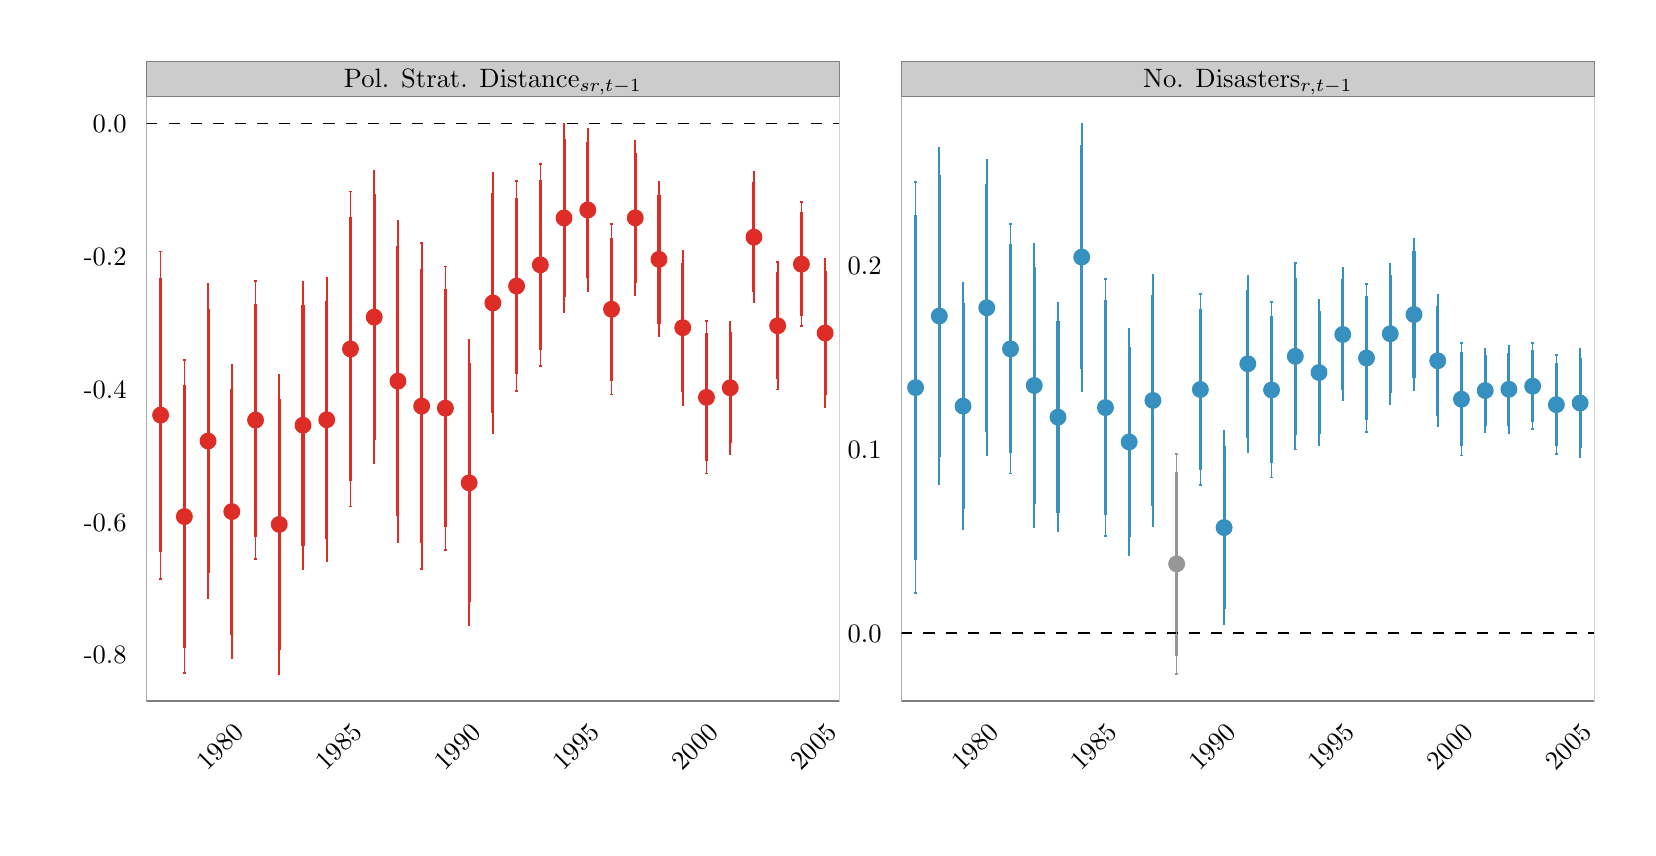
\begin{tikzpicture}[x=1pt,y=1pt]
\definecolor{fillColor}{RGB}{255,255,255}
\path[use as bounding box,fill=fillColor,fill opacity=0.00] (0,0) rectangle (578.16,289.08);
\begin{scope}
\path[clip] (  0.00,  0.00) rectangle (578.16,289.08);
\definecolor{drawColor}{RGB}{255,255,255}
\definecolor{fillColor}{RGB}{255,255,255}

\path[draw=drawColor,line width= 0.6pt,line join=round,line cap=round,fill=fillColor] (  0.00,  0.00) rectangle (578.16,289.08);
\end{scope}
\begin{scope}
\path[clip] ( 42.89, 45.67) rectangle (293.31,264.40);
\definecolor{fillColor}{RGB}{255,255,255}

\path[fill=fillColor] ( 42.89, 45.67) rectangle (293.31,264.40);
\definecolor{drawColor}{RGB}{222,45,38}

\path[draw=drawColor,draw opacity=0.30,line width= 0.3pt,line join=round] ( 48.03, 89.96) -- ( 48.03,208.22);

\path[draw=drawColor,draw opacity=0.30,line width= 0.3pt,line join=round] ( 56.61, 55.94) -- ( 56.61,168.89);

\path[draw=drawColor,draw opacity=0.30,line width= 0.3pt,line join=round] ( 65.18, 82.91) -- ( 65.18,196.49);

\path[draw=drawColor,draw opacity=0.30,line width= 0.3pt,line join=round] ( 73.76, 61.21) -- ( 73.76,167.21);

\path[draw=drawColor,draw opacity=0.30,line width= 0.3pt,line join=round] ( 82.34, 97.13) -- ( 82.34,197.44);

\path[draw=drawColor,draw opacity=0.30,line width= 0.3pt,line join=round] ( 90.91, 55.61) -- ( 90.91,163.55);

\path[draw=drawColor,draw opacity=0.30,line width= 0.3pt,line join=round] ( 99.49, 93.57) -- ( 99.49,197.27);

\path[draw=drawColor,draw opacity=0.30,line width= 0.3pt,line join=round] (108.06, 96.12) -- (108.06,198.68);

\path[draw=drawColor,draw opacity=0.30,line width= 0.3pt,line join=round] (116.64,116.01) -- (116.64,229.92);

\path[draw=drawColor,draw opacity=0.30,line width= 0.3pt,line join=round] (125.22,131.64) -- (125.22,237.35);

\path[draw=drawColor,draw opacity=0.30,line width= 0.3pt,line join=round] (133.79,103.34) -- (133.79,219.35);

\path[draw=drawColor,draw opacity=0.30,line width= 0.3pt,line join=round] (142.37, 93.47) -- (142.37,211.17);

\path[draw=drawColor,draw opacity=0.30,line width= 0.3pt,line join=round] (150.94,100.38) -- (150.94,202.76);

\path[draw=drawColor,draw opacity=0.30,line width= 0.3pt,line join=round] (159.52, 73.11) -- (159.52,176.11);

\path[draw=drawColor,draw opacity=0.30,line width= 0.3pt,line join=round] (168.10,142.41) -- (168.10,236.79);

\path[draw=drawColor,draw opacity=0.30,line width= 0.3pt,line join=round] (176.67,157.86) -- (176.67,233.56);

\path[draw=drawColor,draw opacity=0.30,line width= 0.3pt,line join=round] (185.25,166.82) -- (185.25,239.93);

\path[draw=drawColor,draw opacity=0.30,line width= 0.3pt,line join=round] (193.82,186.38) -- (193.82,254.25);

\path[draw=drawColor,draw opacity=0.30,line width= 0.3pt,line join=round] (202.40,193.76) -- (202.40,252.64);

\path[draw=drawColor,draw opacity=0.30,line width= 0.3pt,line join=round] (210.98,156.50) -- (210.98,218.15);

\path[draw=drawColor,draw opacity=0.30,line width= 0.3pt,line join=round] (219.55,192.41) -- (219.55,248.29);

\path[draw=drawColor,draw opacity=0.30,line width= 0.3pt,line join=round] (228.13,177.46) -- (228.13,233.26);

\path[draw=drawColor,draw opacity=0.30,line width= 0.3pt,line join=round] (236.70,152.79) -- (236.70,208.56);

\path[draw=drawColor,draw opacity=0.30,line width= 0.3pt,line join=round] (245.28,127.96) -- (245.28,183.01);

\path[draw=drawColor,draw opacity=0.30,line width= 0.3pt,line join=round] (253.86,135.12) -- (253.86,182.76);

\path[draw=drawColor,draw opacity=0.30,line width= 0.3pt,line join=round] (262.43,189.73) -- (262.43,237.05);

\path[draw=drawColor,draw opacity=0.30,line width= 0.3pt,line join=round] (271.01,158.31) -- (271.01,204.38);

\path[draw=drawColor,draw opacity=0.30,line width= 0.3pt,line join=round] (279.58,181.27) -- (279.58,225.98);

\path[draw=drawColor,draw opacity=0.30,line width= 0.3pt,line join=round] (288.16,151.94) -- (288.16,205.54);
\definecolor{drawColor}{RGB}{222,45,38}

\path[draw=drawColor,line width= 1.1pt,line join=round] ( 48.03, 99.47) -- ( 48.03,198.71);

\path[draw=drawColor,line width= 1.1pt,line join=round] ( 56.61, 65.02) -- ( 56.61,159.81);

\path[draw=drawColor,line width= 1.1pt,line join=round] ( 65.18, 92.04) -- ( 65.18,187.36);

\path[draw=drawColor,line width= 1.1pt,line join=round] ( 73.76, 69.73) -- ( 73.76,158.69);

\path[draw=drawColor,line width= 1.1pt,line join=round] ( 82.34,105.19) -- ( 82.34,189.38);

\path[draw=drawColor,line width= 1.1pt,line join=round] ( 90.91, 64.29) -- ( 90.91,154.88);

\path[draw=drawColor,line width= 1.1pt,line join=round] ( 99.49,101.91) -- ( 99.49,188.94);

\path[draw=drawColor,line width= 1.1pt,line join=round] (108.06,104.37) -- (108.06,190.44);

\path[draw=drawColor,line width= 1.1pt,line join=round] (116.64,125.16) -- (116.64,220.77);

\path[draw=drawColor,line width= 1.1pt,line join=round] (125.22,140.14) -- (125.22,228.85);

\path[draw=drawColor,line width= 1.1pt,line join=round] (133.79,112.67) -- (133.79,210.03);

\path[draw=drawColor,line width= 1.1pt,line join=round] (142.37,102.93) -- (142.37,201.71);

\path[draw=drawColor,line width= 1.1pt,line join=round] (150.94,108.61) -- (150.94,194.53);

\path[draw=drawColor,line width= 1.1pt,line join=round] (159.52, 81.39) -- (159.52,167.83);

\path[draw=drawColor,line width= 1.1pt,line join=round] (168.10,149.99) -- (168.10,229.21);

\path[draw=drawColor,line width= 1.1pt,line join=round] (176.67,163.95) -- (176.67,227.47);

\path[draw=drawColor,line width= 1.1pt,line join=round] (185.25,172.69) -- (185.25,234.05);

\path[draw=drawColor,line width= 1.1pt,line join=round] (193.82,191.84) -- (193.82,248.79);

\path[draw=drawColor,line width= 1.1pt,line join=round] (202.40,198.50) -- (202.40,247.91);

\path[draw=drawColor,line width= 1.1pt,line join=round] (210.98,161.46) -- (210.98,213.19);

\path[draw=drawColor,line width= 1.1pt,line join=round] (219.55,196.90) -- (219.55,243.80);

\path[draw=drawColor,line width= 1.1pt,line join=round] (228.13,181.94) -- (228.13,228.78);

\path[draw=drawColor,line width= 1.1pt,line join=round] (236.70,157.27) -- (236.70,204.08);

\path[draw=drawColor,line width= 1.1pt,line join=round] (245.28,132.39) -- (245.28,178.59);

\path[draw=drawColor,line width= 1.1pt,line join=round] (253.86,138.95) -- (253.86,178.93);

\path[draw=drawColor,line width= 1.1pt,line join=round] (262.43,193.54) -- (262.43,233.25);

\path[draw=drawColor,line width= 1.1pt,line join=round] (271.01,162.01) -- (271.01,200.68);

\path[draw=drawColor,line width= 1.1pt,line join=round] (279.58,184.86) -- (279.58,222.39);

\path[draw=drawColor,line width= 1.1pt,line join=round] (288.16,156.25) -- (288.16,201.23);
\definecolor{drawColor}{RGB}{0,0,0}

\path[draw=drawColor,line width= 0.6pt,dash pattern=on 4pt off 4pt ,line join=round] ( 42.89,254.46) -- (293.31,254.46);
\definecolor{drawColor}{RGB}{222,45,38}
\definecolor{fillColor}{RGB}{222,45,38}

\path[draw=drawColor,line width= 0.4pt,line join=round,line cap=round,fill=fillColor] ( 48.03,149.09) circle (  2.85);

\path[draw=drawColor,line width= 0.4pt,line join=round,line cap=round,fill=fillColor] ( 56.61,112.42) circle (  2.85);

\path[draw=drawColor,line width= 0.4pt,line join=round,line cap=round,fill=fillColor] ( 65.18,139.70) circle (  2.85);

\path[draw=drawColor,line width= 0.4pt,line join=round,line cap=round,fill=fillColor] ( 73.76,114.21) circle (  2.85);

\path[draw=drawColor,line width= 0.4pt,line join=round,line cap=round,fill=fillColor] ( 82.34,147.29) circle (  2.85);

\path[draw=drawColor,line width= 0.4pt,line join=round,line cap=round,fill=fillColor] ( 90.91,109.58) circle (  2.85);

\path[draw=drawColor,line width= 0.4pt,line join=round,line cap=round,fill=fillColor] ( 99.49,145.42) circle (  2.85);

\path[draw=drawColor,line width= 0.4pt,line join=round,line cap=round,fill=fillColor] (108.06,147.40) circle (  2.85);

\path[draw=drawColor,line width= 0.4pt,line join=round,line cap=round,fill=fillColor] (116.64,172.97) circle (  2.85);

\path[draw=drawColor,line width= 0.4pt,line join=round,line cap=round,fill=fillColor] (125.22,184.49) circle (  2.85);

\path[draw=drawColor,line width= 0.4pt,line join=round,line cap=round,fill=fillColor] (133.79,161.35) circle (  2.85);

\path[draw=drawColor,line width= 0.4pt,line join=round,line cap=round,fill=fillColor] (142.37,152.32) circle (  2.85);

\path[draw=drawColor,line width= 0.4pt,line join=round,line cap=round,fill=fillColor] (150.94,151.57) circle (  2.85);

\path[draw=drawColor,line width= 0.4pt,line join=round,line cap=round,fill=fillColor] (159.52,124.61) circle (  2.85);

\path[draw=drawColor,line width= 0.4pt,line join=round,line cap=round,fill=fillColor] (168.10,189.60) circle (  2.85);

\path[draw=drawColor,line width= 0.4pt,line join=round,line cap=round,fill=fillColor] (176.67,195.71) circle (  2.85);

\path[draw=drawColor,line width= 0.4pt,line join=round,line cap=round,fill=fillColor] (185.25,203.37) circle (  2.85);

\path[draw=drawColor,line width= 0.4pt,line join=round,line cap=round,fill=fillColor] (193.82,220.32) circle (  2.85);

\path[draw=drawColor,line width= 0.4pt,line join=round,line cap=round,fill=fillColor] (202.40,223.20) circle (  2.85);

\path[draw=drawColor,line width= 0.4pt,line join=round,line cap=round,fill=fillColor] (210.98,187.33) circle (  2.85);

\path[draw=drawColor,line width= 0.4pt,line join=round,line cap=round,fill=fillColor] (219.55,220.35) circle (  2.85);

\path[draw=drawColor,line width= 0.4pt,line join=round,line cap=round,fill=fillColor] (228.13,205.36) circle (  2.85);

\path[draw=drawColor,line width= 0.4pt,line join=round,line cap=round,fill=fillColor] (236.70,180.67) circle (  2.85);

\path[draw=drawColor,line width= 0.4pt,line join=round,line cap=round,fill=fillColor] (245.28,155.49) circle (  2.85);

\path[draw=drawColor,line width= 0.4pt,line join=round,line cap=round,fill=fillColor] (253.86,158.94) circle (  2.85);

\path[draw=drawColor,line width= 0.4pt,line join=round,line cap=round,fill=fillColor] (262.43,213.39) circle (  2.85);

\path[draw=drawColor,line width= 0.4pt,line join=round,line cap=round,fill=fillColor] (271.01,181.35) circle (  2.85);

\path[draw=drawColor,line width= 0.4pt,line join=round,line cap=round,fill=fillColor] (279.58,203.62) circle (  2.85);

\path[draw=drawColor,line width= 0.4pt,line join=round,line cap=round,fill=fillColor] (288.16,178.74) circle (  2.85);

\path[draw=drawColor,line width= 0.6pt,line join=round] ( 47.60,208.22) --
	( 48.46,208.22);

\path[draw=drawColor,line width= 0.6pt,line join=round] ( 48.03,208.22) --
	( 48.03, 89.96);

\path[draw=drawColor,line width= 0.6pt,line join=round] ( 47.60, 89.96) --
	( 48.46, 89.96);

\path[draw=drawColor,line width= 0.6pt,line join=round] ( 56.18,168.89) --
	( 57.04,168.89);

\path[draw=drawColor,line width= 0.6pt,line join=round] ( 56.61,168.89) --
	( 56.61, 55.94);

\path[draw=drawColor,line width= 0.6pt,line join=round] ( 56.18, 55.94) --
	( 57.04, 55.94);

\path[draw=drawColor,line width= 0.6pt,line join=round] ( 64.75,196.49) --
	( 65.61,196.49);

\path[draw=drawColor,line width= 0.6pt,line join=round] ( 65.18,196.49) --
	( 65.18, 82.91);

\path[draw=drawColor,line width= 0.6pt,line join=round] ( 64.75, 82.91) --
	( 65.61, 82.91);

\path[draw=drawColor,line width= 0.6pt,line join=round] ( 73.33,167.21) --
	( 74.19,167.21);

\path[draw=drawColor,line width= 0.6pt,line join=round] ( 73.76,167.21) --
	( 73.76, 61.21);

\path[draw=drawColor,line width= 0.6pt,line join=round] ( 73.33, 61.21) --
	( 74.19, 61.21);

\path[draw=drawColor,line width= 0.6pt,line join=round] ( 81.91,197.44) --
	( 82.76,197.44);

\path[draw=drawColor,line width= 0.6pt,line join=round] ( 82.34,197.44) --
	( 82.34, 97.13);

\path[draw=drawColor,line width= 0.6pt,line join=round] ( 81.91, 97.13) --
	( 82.76, 97.13);

\path[draw=drawColor,line width= 0.6pt,line join=round] ( 90.48,163.55) --
	( 91.34,163.55);

\path[draw=drawColor,line width= 0.6pt,line join=round] ( 90.91,163.55) --
	( 90.91, 55.61);

\path[draw=drawColor,line width= 0.6pt,line join=round] ( 90.48, 55.61) --
	( 91.34, 55.61);

\path[draw=drawColor,line width= 0.6pt,line join=round] ( 99.06,197.27) --
	( 99.92,197.27);

\path[draw=drawColor,line width= 0.6pt,line join=round] ( 99.49,197.27) --
	( 99.49, 93.57);

\path[draw=drawColor,line width= 0.6pt,line join=round] ( 99.06, 93.57) --
	( 99.92, 93.57);

\path[draw=drawColor,line width= 0.6pt,line join=round] (107.63,198.68) --
	(108.49,198.68);

\path[draw=drawColor,line width= 0.6pt,line join=round] (108.06,198.68) --
	(108.06, 96.12);

\path[draw=drawColor,line width= 0.6pt,line join=round] (107.63, 96.12) --
	(108.49, 96.12);

\path[draw=drawColor,line width= 0.6pt,line join=round] (116.21,229.92) --
	(117.07,229.92);

\path[draw=drawColor,line width= 0.6pt,line join=round] (116.64,229.92) --
	(116.64,116.01);

\path[draw=drawColor,line width= 0.6pt,line join=round] (116.21,116.01) --
	(117.07,116.01);

\path[draw=drawColor,line width= 0.6pt,line join=round] (124.79,237.35) --
	(125.64,237.35);

\path[draw=drawColor,line width= 0.6pt,line join=round] (125.22,237.35) --
	(125.22,131.64);

\path[draw=drawColor,line width= 0.6pt,line join=round] (124.79,131.64) --
	(125.64,131.64);

\path[draw=drawColor,line width= 0.6pt,line join=round] (133.36,219.35) --
	(134.22,219.35);

\path[draw=drawColor,line width= 0.6pt,line join=round] (133.79,219.35) --
	(133.79,103.34);

\path[draw=drawColor,line width= 0.6pt,line join=round] (133.36,103.34) --
	(134.22,103.34);

\path[draw=drawColor,line width= 0.6pt,line join=round] (141.94,211.17) --
	(142.80,211.17);

\path[draw=drawColor,line width= 0.6pt,line join=round] (142.37,211.17) --
	(142.37, 93.47);

\path[draw=drawColor,line width= 0.6pt,line join=round] (141.94, 93.47) --
	(142.80, 93.47);

\path[draw=drawColor,line width= 0.6pt,line join=round] (150.52,202.76) --
	(151.37,202.76);

\path[draw=drawColor,line width= 0.6pt,line join=round] (150.94,202.76) --
	(150.94,100.38);

\path[draw=drawColor,line width= 0.6pt,line join=round] (150.52,100.38) --
	(151.37,100.38);

\path[draw=drawColor,line width= 0.6pt,line join=round] (159.09,176.11) --
	(159.95,176.11);

\path[draw=drawColor,line width= 0.6pt,line join=round] (159.52,176.11) --
	(159.52, 73.11);

\path[draw=drawColor,line width= 0.6pt,line join=round] (159.09, 73.11) --
	(159.95, 73.11);

\path[draw=drawColor,line width= 0.6pt,line join=round] (167.67,236.79) --
	(168.52,236.79);

\path[draw=drawColor,line width= 0.6pt,line join=round] (168.10,236.79) --
	(168.10,142.41);

\path[draw=drawColor,line width= 0.6pt,line join=round] (167.67,142.41) --
	(168.52,142.41);

\path[draw=drawColor,line width= 0.6pt,line join=round] (176.24,233.56) --
	(177.10,233.56);

\path[draw=drawColor,line width= 0.6pt,line join=round] (176.67,233.56) --
	(176.67,157.86);

\path[draw=drawColor,line width= 0.6pt,line join=round] (176.24,157.86) --
	(177.10,157.86);

\path[draw=drawColor,line width= 0.6pt,line join=round] (184.82,239.93) --
	(185.68,239.93);

\path[draw=drawColor,line width= 0.6pt,line join=round] (185.25,239.93) --
	(185.25,166.82);

\path[draw=drawColor,line width= 0.6pt,line join=round] (184.82,166.82) --
	(185.68,166.82);

\path[draw=drawColor,line width= 0.6pt,line join=round] (193.40,254.25) --
	(194.25,254.25);

\path[draw=drawColor,line width= 0.6pt,line join=round] (193.82,254.25) --
	(193.82,186.38);

\path[draw=drawColor,line width= 0.6pt,line join=round] (193.40,186.38) --
	(194.25,186.38);

\path[draw=drawColor,line width= 0.6pt,line join=round] (201.97,252.64) --
	(202.83,252.64);

\path[draw=drawColor,line width= 0.6pt,line join=round] (202.40,252.64) --
	(202.40,193.76);

\path[draw=drawColor,line width= 0.6pt,line join=round] (201.97,193.76) --
	(202.83,193.76);

\path[draw=drawColor,line width= 0.6pt,line join=round] (210.55,218.15) --
	(211.41,218.15);

\path[draw=drawColor,line width= 0.6pt,line join=round] (210.98,218.15) --
	(210.98,156.50);

\path[draw=drawColor,line width= 0.6pt,line join=round] (210.55,156.50) --
	(211.41,156.50);

\path[draw=drawColor,line width= 0.6pt,line join=round] (219.12,248.29) --
	(219.98,248.29);

\path[draw=drawColor,line width= 0.6pt,line join=round] (219.55,248.29) --
	(219.55,192.41);

\path[draw=drawColor,line width= 0.6pt,line join=round] (219.12,192.41) --
	(219.98,192.41);

\path[draw=drawColor,line width= 0.6pt,line join=round] (227.70,233.26) --
	(228.56,233.26);

\path[draw=drawColor,line width= 0.6pt,line join=round] (228.13,233.26) --
	(228.13,177.46);

\path[draw=drawColor,line width= 0.6pt,line join=round] (227.70,177.46) --
	(228.56,177.46);

\path[draw=drawColor,line width= 0.6pt,line join=round] (236.28,208.56) --
	(237.13,208.56);

\path[draw=drawColor,line width= 0.6pt,line join=round] (236.70,208.56) --
	(236.70,152.79);

\path[draw=drawColor,line width= 0.6pt,line join=round] (236.28,152.79) --
	(237.13,152.79);

\path[draw=drawColor,line width= 0.6pt,line join=round] (244.85,183.01) --
	(245.71,183.01);

\path[draw=drawColor,line width= 0.6pt,line join=round] (245.28,183.01) --
	(245.28,127.96);

\path[draw=drawColor,line width= 0.6pt,line join=round] (244.85,127.96) --
	(245.71,127.96);

\path[draw=drawColor,line width= 0.6pt,line join=round] (253.43,182.76) --
	(254.29,182.76);

\path[draw=drawColor,line width= 0.6pt,line join=round] (253.86,182.76) --
	(253.86,135.12);

\path[draw=drawColor,line width= 0.6pt,line join=round] (253.43,135.12) --
	(254.29,135.12);

\path[draw=drawColor,line width= 0.6pt,line join=round] (262.00,237.05) --
	(262.86,237.05);

\path[draw=drawColor,line width= 0.6pt,line join=round] (262.43,237.05) --
	(262.43,189.73);

\path[draw=drawColor,line width= 0.6pt,line join=round] (262.00,189.73) --
	(262.86,189.73);

\path[draw=drawColor,line width= 0.6pt,line join=round] (270.58,204.38) --
	(271.44,204.38);

\path[draw=drawColor,line width= 0.6pt,line join=round] (271.01,204.38) --
	(271.01,158.31);

\path[draw=drawColor,line width= 0.6pt,line join=round] (270.58,158.31) --
	(271.44,158.31);

\path[draw=drawColor,line width= 0.6pt,line join=round] (279.16,225.98) --
	(280.01,225.98);

\path[draw=drawColor,line width= 0.6pt,line join=round] (279.58,225.98) --
	(279.58,181.27);

\path[draw=drawColor,line width= 0.6pt,line join=round] (279.16,181.27) --
	(280.01,181.27);

\path[draw=drawColor,line width= 0.6pt,line join=round] (287.73,205.54) --
	(288.59,205.54);

\path[draw=drawColor,line width= 0.6pt,line join=round] (288.16,205.54) --
	(288.16,151.94);

\path[draw=drawColor,line width= 0.6pt,line join=round] (287.73,151.94) --
	(288.59,151.94);
\definecolor{drawColor}{gray}{0.50}

\path[draw=drawColor,line width= 0.6pt,line join=round,line cap=round] ( 42.89, 45.67) rectangle (293.31,264.40);
\end{scope}
\begin{scope}
\path[clip] (315.69, 45.67) rectangle (566.12,264.40);
\definecolor{fillColor}{RGB}{255,255,255}

\path[fill=fillColor] (315.69, 45.67) rectangle (566.12,264.40);
\definecolor{drawColor}{RGB}{54,144,192}

\path[draw=drawColor,draw opacity=0.30,line width= 0.3pt,line join=round] (320.84, 84.78) -- (320.84,233.26);

\path[draw=drawColor,draw opacity=0.30,line width= 0.3pt,line join=round] (329.42,124.20) -- (329.42,245.58);

\path[draw=drawColor,draw opacity=0.30,line width= 0.3pt,line join=round] (337.99,107.85) -- (337.99,196.79);

\path[draw=drawColor,draw opacity=0.30,line width= 0.3pt,line join=round] (346.57,134.53) -- (346.57,241.19);

\path[draw=drawColor,draw opacity=0.30,line width= 0.3pt,line join=round] (355.14,128.00) -- (355.14,218.02);

\path[draw=drawColor,draw opacity=0.30,line width= 0.3pt,line join=round] (363.72,108.61) -- (363.72,210.96);

\path[draw=drawColor,draw opacity=0.30,line width= 0.3pt,line join=round] (372.30,107.10) -- (372.30,189.58);

\path[draw=drawColor,draw opacity=0.30,line width= 0.3pt,line join=round] (380.87,157.89) -- (380.87,254.46);

\path[draw=drawColor,draw opacity=0.30,line width= 0.3pt,line join=round] (389.45,105.38) -- (389.45,198.20);

\path[draw=drawColor,draw opacity=0.30,line width= 0.3pt,line join=round] (398.02, 98.44) -- (398.02,180.32);

\path[draw=drawColor,draw opacity=0.30,line width= 0.3pt,line join=round] (406.60,108.83) -- (406.60,199.93);
\definecolor{drawColor}{RGB}{150,150,150}

\path[draw=drawColor,draw opacity=0.30,line width= 0.3pt,line join=round] (415.18, 55.61) -- (415.18,135.03);
\definecolor{drawColor}{RGB}{54,144,192}

\path[draw=drawColor,draw opacity=0.30,line width= 0.3pt,line join=round] (423.75,123.82) -- (423.75,192.84);

\path[draw=drawColor,draw opacity=0.30,line width= 0.3pt,line join=round] (432.33, 73.48) -- (432.33,143.39);

\path[draw=drawColor,draw opacity=0.30,line width= 0.3pt,line join=round] (440.90,135.71) -- (440.90,199.57);

\path[draw=drawColor,draw opacity=0.30,line width= 0.3pt,line join=round] (449.48,126.51) -- (449.48,189.85);

\path[draw=drawColor,draw opacity=0.30,line width= 0.3pt,line join=round] (458.06,136.62) -- (458.06,204.01);

\path[draw=drawColor,draw opacity=0.30,line width= 0.3pt,line join=round] (466.63,138.09) -- (466.63,190.85);

\path[draw=drawColor,draw opacity=0.30,line width= 0.3pt,line join=round] (475.21,154.32) -- (475.21,202.12);

\path[draw=drawColor,draw opacity=0.30,line width= 0.3pt,line join=round] (483.78,143.07) -- (483.78,196.36);

\path[draw=drawColor,draw opacity=0.30,line width= 0.3pt,line join=round] (492.36,153.05) -- (492.36,203.91);

\path[draw=drawColor,draw opacity=0.30,line width= 0.3pt,line join=round] (500.94,158.05) -- (500.94,212.80);

\path[draw=drawColor,draw opacity=0.30,line width= 0.3pt,line join=round] (509.51,145.03) -- (509.51,192.41);

\path[draw=drawColor,draw opacity=0.30,line width= 0.3pt,line join=round] (518.09,134.49) -- (518.09,175.12);

\path[draw=drawColor,draw opacity=0.30,line width= 0.3pt,line join=round] (526.67,142.74) -- (526.67,173.16);

\path[draw=drawColor,draw opacity=0.30,line width= 0.3pt,line join=round] (535.24,142.56) -- (535.24,174.24);

\path[draw=drawColor,draw opacity=0.30,line width= 0.3pt,line join=round] (543.82,143.99) -- (543.82,175.07);

\path[draw=drawColor,draw opacity=0.30,line width= 0.3pt,line join=round] (552.39,134.95) -- (552.39,170.75);

\path[draw=drawColor,draw opacity=0.30,line width= 0.3pt,line join=round] (560.97,134.02) -- (560.97,172.88);
\definecolor{drawColor}{RGB}{54,144,192}

\path[draw=drawColor,line width= 1.1pt,line join=round] (320.84, 96.72) -- (320.84,221.32);

\path[draw=drawColor,line width= 1.1pt,line join=round] (329.42,133.96) -- (329.42,235.83);

\path[draw=drawColor,line width= 1.1pt,line join=round] (337.99,115.00) -- (337.99,189.64);

\path[draw=drawColor,line width= 1.1pt,line join=round] (346.57,143.11) -- (346.57,232.62);

\path[draw=drawColor,line width= 1.1pt,line join=round] (355.14,135.23) -- (355.14,210.79);

\path[draw=drawColor,line width= 1.1pt,line join=round] (363.72,116.84) -- (363.72,202.73);

\path[draw=drawColor,line width= 1.1pt,line join=round] (372.30,113.73) -- (372.30,182.95);

\path[draw=drawColor,line width= 1.1pt,line join=round] (380.87,165.65) -- (380.87,246.70);

\path[draw=drawColor,line width= 1.1pt,line join=round] (389.45,112.84) -- (389.45,190.74);

\path[draw=drawColor,line width= 1.1pt,line join=round] (398.02,105.02) -- (398.02,173.74);

\path[draw=drawColor,line width= 1.1pt,line join=round] (406.60,116.15) -- (406.60,192.61);
\definecolor{drawColor}{gray}{0.59}

\path[draw=drawColor,line width= 1.1pt,line join=round] (415.18, 62.00) -- (415.18,128.64);
\definecolor{drawColor}{RGB}{54,144,192}

\path[draw=drawColor,line width= 1.1pt,line join=round] (423.75,129.37) -- (423.75,187.29);

\path[draw=drawColor,line width= 1.1pt,line join=round] (432.33, 79.10) -- (432.33,137.77);

\path[draw=drawColor,line width= 1.1pt,line join=round] (440.90,140.84) -- (440.90,194.44);

\path[draw=drawColor,line width= 1.1pt,line join=round] (449.48,131.60) -- (449.48,184.76);

\path[draw=drawColor,line width= 1.1pt,line join=round] (458.06,142.04) -- (458.06,198.59);

\path[draw=drawColor,line width= 1.1pt,line join=round] (466.63,142.33) -- (466.63,186.61);

\path[draw=drawColor,line width= 1.1pt,line join=round] (475.21,158.17) -- (475.21,198.28);

\path[draw=drawColor,line width= 1.1pt,line join=round] (483.78,147.36) -- (483.78,192.07);

\path[draw=drawColor,line width= 1.1pt,line join=round] (492.36,157.14) -- (492.36,199.82);

\path[draw=drawColor,line width= 1.1pt,line join=round] (500.94,162.45) -- (500.94,208.40);

\path[draw=drawColor,line width= 1.1pt,line join=round] (509.51,148.84) -- (509.51,188.60);

\path[draw=drawColor,line width= 1.1pt,line join=round] (518.09,137.76) -- (518.09,171.86);

\path[draw=drawColor,line width= 1.1pt,line join=round] (526.67,145.19) -- (526.67,170.71);

\path[draw=drawColor,line width= 1.1pt,line join=round] (535.24,145.11) -- (535.24,171.69);

\path[draw=drawColor,line width= 1.1pt,line join=round] (543.82,146.49) -- (543.82,172.57);

\path[draw=drawColor,line width= 1.1pt,line join=round] (552.39,137.83) -- (552.39,167.87);

\path[draw=drawColor,line width= 1.1pt,line join=round] (560.97,137.14) -- (560.97,169.75);
\definecolor{drawColor}{RGB}{0,0,0}

\path[draw=drawColor,line width= 0.6pt,dash pattern=on 4pt off 4pt ,line join=round] (315.69, 70.25) -- (566.12, 70.25);
\definecolor{drawColor}{RGB}{54,144,192}
\definecolor{fillColor}{RGB}{54,144,192}

\path[draw=drawColor,line width= 0.4pt,line join=round,line cap=round,fill=fillColor] (320.84,159.02) circle (  2.85);

\path[draw=drawColor,line width= 0.4pt,line join=round,line cap=round,fill=fillColor] (329.42,184.89) circle (  2.85);

\path[draw=drawColor,line width= 0.4pt,line join=round,line cap=round,fill=fillColor] (337.99,152.32) circle (  2.85);

\path[draw=drawColor,line width= 0.4pt,line join=round,line cap=round,fill=fillColor] (346.57,187.86) circle (  2.85);

\path[draw=drawColor,line width= 0.4pt,line join=round,line cap=round,fill=fillColor] (355.14,173.01) circle (  2.85);

\path[draw=drawColor,line width= 0.4pt,line join=round,line cap=round,fill=fillColor] (363.72,159.79) circle (  2.85);

\path[draw=drawColor,line width= 0.4pt,line join=round,line cap=round,fill=fillColor] (372.30,148.34) circle (  2.85);

\path[draw=drawColor,line width= 0.4pt,line join=round,line cap=round,fill=fillColor] (380.87,206.17) circle (  2.85);

\path[draw=drawColor,line width= 0.4pt,line join=round,line cap=round,fill=fillColor] (389.45,151.79) circle (  2.85);

\path[draw=drawColor,line width= 0.4pt,line join=round,line cap=round,fill=fillColor] (398.02,139.38) circle (  2.85);

\path[draw=drawColor,line width= 0.4pt,line join=round,line cap=round,fill=fillColor] (406.60,154.38) circle (  2.85);
\definecolor{drawColor}{gray}{0.59}
\definecolor{fillColor}{gray}{0.59}

\path[draw=drawColor,line width= 0.4pt,line join=round,line cap=round,fill=fillColor] (415.18, 95.32) circle (  2.85);
\definecolor{drawColor}{RGB}{54,144,192}
\definecolor{fillColor}{RGB}{54,144,192}

\path[draw=drawColor,line width= 0.4pt,line join=round,line cap=round,fill=fillColor] (423.75,158.33) circle (  2.85);

\path[draw=drawColor,line width= 0.4pt,line join=round,line cap=round,fill=fillColor] (432.33,108.43) circle (  2.85);

\path[draw=drawColor,line width= 0.4pt,line join=round,line cap=round,fill=fillColor] (440.90,167.64) circle (  2.85);

\path[draw=drawColor,line width= 0.4pt,line join=round,line cap=round,fill=fillColor] (449.48,158.18) circle (  2.85);

\path[draw=drawColor,line width= 0.4pt,line join=round,line cap=round,fill=fillColor] (458.06,170.32) circle (  2.85);

\path[draw=drawColor,line width= 0.4pt,line join=round,line cap=round,fill=fillColor] (466.63,164.47) circle (  2.85);

\path[draw=drawColor,line width= 0.4pt,line join=round,line cap=round,fill=fillColor] (475.21,178.22) circle (  2.85);

\path[draw=drawColor,line width= 0.4pt,line join=round,line cap=round,fill=fillColor] (483.78,169.72) circle (  2.85);

\path[draw=drawColor,line width= 0.4pt,line join=round,line cap=round,fill=fillColor] (492.36,178.48) circle (  2.85);

\path[draw=drawColor,line width= 0.4pt,line join=round,line cap=round,fill=fillColor] (500.94,185.42) circle (  2.85);

\path[draw=drawColor,line width= 0.4pt,line join=round,line cap=round,fill=fillColor] (509.51,168.72) circle (  2.85);

\path[draw=drawColor,line width= 0.4pt,line join=round,line cap=round,fill=fillColor] (518.09,154.81) circle (  2.85);

\path[draw=drawColor,line width= 0.4pt,line join=round,line cap=round,fill=fillColor] (526.67,157.95) circle (  2.85);

\path[draw=drawColor,line width= 0.4pt,line join=round,line cap=round,fill=fillColor] (535.24,158.40) circle (  2.85);

\path[draw=drawColor,line width= 0.4pt,line join=round,line cap=round,fill=fillColor] (543.82,159.53) circle (  2.85);

\path[draw=drawColor,line width= 0.4pt,line join=round,line cap=round,fill=fillColor] (552.39,152.85) circle (  2.85);

\path[draw=drawColor,line width= 0.4pt,line join=round,line cap=round,fill=fillColor] (560.97,153.45) circle (  2.85);

\path[draw=drawColor,line width= 0.6pt,line join=round] (320.41,233.26) --
	(321.27,233.26);

\path[draw=drawColor,line width= 0.6pt,line join=round] (320.84,233.26) --
	(320.84, 84.78);

\path[draw=drawColor,line width= 0.6pt,line join=round] (320.41, 84.78) --
	(321.27, 84.78);

\path[draw=drawColor,line width= 0.6pt,line join=round] (328.99,245.58) --
	(329.84,245.58);

\path[draw=drawColor,line width= 0.6pt,line join=round] (329.42,245.58) --
	(329.42,124.20);

\path[draw=drawColor,line width= 0.6pt,line join=round] (328.99,124.20) --
	(329.84,124.20);

\path[draw=drawColor,line width= 0.6pt,line join=round] (337.56,196.79) --
	(338.42,196.79);

\path[draw=drawColor,line width= 0.6pt,line join=round] (337.99,196.79) --
	(337.99,107.85);

\path[draw=drawColor,line width= 0.6pt,line join=round] (337.56,107.85) --
	(338.42,107.85);

\path[draw=drawColor,line width= 0.6pt,line join=round] (346.14,241.19) --
	(347.00,241.19);

\path[draw=drawColor,line width= 0.6pt,line join=round] (346.57,241.19) --
	(346.57,134.53);

\path[draw=drawColor,line width= 0.6pt,line join=round] (346.14,134.53) --
	(347.00,134.53);

\path[draw=drawColor,line width= 0.6pt,line join=round] (354.72,218.02) --
	(355.57,218.02);

\path[draw=drawColor,line width= 0.6pt,line join=round] (355.14,218.02) --
	(355.14,128.00);

\path[draw=drawColor,line width= 0.6pt,line join=round] (354.72,128.00) --
	(355.57,128.00);

\path[draw=drawColor,line width= 0.6pt,line join=round] (363.29,210.96) --
	(364.15,210.96);

\path[draw=drawColor,line width= 0.6pt,line join=round] (363.72,210.96) --
	(363.72,108.61);

\path[draw=drawColor,line width= 0.6pt,line join=round] (363.29,108.61) --
	(364.15,108.61);

\path[draw=drawColor,line width= 0.6pt,line join=round] (371.87,189.58) --
	(372.73,189.58);

\path[draw=drawColor,line width= 0.6pt,line join=round] (372.30,189.58) --
	(372.30,107.10);

\path[draw=drawColor,line width= 0.6pt,line join=round] (371.87,107.10) --
	(372.73,107.10);

\path[draw=drawColor,line width= 0.6pt,line join=round] (380.44,254.46) --
	(381.30,254.46);

\path[draw=drawColor,line width= 0.6pt,line join=round] (380.87,254.46) --
	(380.87,157.89);

\path[draw=drawColor,line width= 0.6pt,line join=round] (380.44,157.89) --
	(381.30,157.89);

\path[draw=drawColor,line width= 0.6pt,line join=round] (389.02,198.20) --
	(389.88,198.20);

\path[draw=drawColor,line width= 0.6pt,line join=round] (389.45,198.20) --
	(389.45,105.38);

\path[draw=drawColor,line width= 0.6pt,line join=round] (389.02,105.38) --
	(389.88,105.38);

\path[draw=drawColor,line width= 0.6pt,line join=round] (397.60,180.32) --
	(398.45,180.32);

\path[draw=drawColor,line width= 0.6pt,line join=round] (398.02,180.32) --
	(398.02, 98.44);

\path[draw=drawColor,line width= 0.6pt,line join=round] (397.60, 98.44) --
	(398.45, 98.44);

\path[draw=drawColor,line width= 0.6pt,line join=round] (406.17,199.93) --
	(407.03,199.93);

\path[draw=drawColor,line width= 0.6pt,line join=round] (406.60,199.93) --
	(406.60,108.83);

\path[draw=drawColor,line width= 0.6pt,line join=round] (406.17,108.83) --
	(407.03,108.83);
\definecolor{drawColor}{gray}{0.59}

\path[draw=drawColor,line width= 0.6pt,line join=round] (414.75,135.03) --
	(415.61,135.03);

\path[draw=drawColor,line width= 0.6pt,line join=round] (415.18,135.03) --
	(415.18, 55.61);

\path[draw=drawColor,line width= 0.6pt,line join=round] (414.75, 55.61) --
	(415.61, 55.61);
\definecolor{drawColor}{RGB}{54,144,192}

\path[draw=drawColor,line width= 0.6pt,line join=round] (423.32,192.84) --
	(424.18,192.84);

\path[draw=drawColor,line width= 0.6pt,line join=round] (423.75,192.84) --
	(423.75,123.82);

\path[draw=drawColor,line width= 0.6pt,line join=round] (423.32,123.82) --
	(424.18,123.82);

\path[draw=drawColor,line width= 0.6pt,line join=round] (431.90,143.39) --
	(432.76,143.39);

\path[draw=drawColor,line width= 0.6pt,line join=round] (432.33,143.39) --
	(432.33, 73.48);

\path[draw=drawColor,line width= 0.6pt,line join=round] (431.90, 73.48) --
	(432.76, 73.48);

\path[draw=drawColor,line width= 0.6pt,line join=round] (440.48,199.57) --
	(441.33,199.57);

\path[draw=drawColor,line width= 0.6pt,line join=round] (440.90,199.57) --
	(440.90,135.71);

\path[draw=drawColor,line width= 0.6pt,line join=round] (440.48,135.71) --
	(441.33,135.71);

\path[draw=drawColor,line width= 0.6pt,line join=round] (449.05,189.85) --
	(449.91,189.85);

\path[draw=drawColor,line width= 0.6pt,line join=round] (449.48,189.85) --
	(449.48,126.51);

\path[draw=drawColor,line width= 0.6pt,line join=round] (449.05,126.51) --
	(449.91,126.51);

\path[draw=drawColor,line width= 0.6pt,line join=round] (457.63,204.01) --
	(458.49,204.01);

\path[draw=drawColor,line width= 0.6pt,line join=round] (458.06,204.01) --
	(458.06,136.62);

\path[draw=drawColor,line width= 0.6pt,line join=round] (457.63,136.62) --
	(458.49,136.62);

\path[draw=drawColor,line width= 0.6pt,line join=round] (466.20,190.85) --
	(467.06,190.85);

\path[draw=drawColor,line width= 0.6pt,line join=round] (466.63,190.85) --
	(466.63,138.09);

\path[draw=drawColor,line width= 0.6pt,line join=round] (466.20,138.09) --
	(467.06,138.09);

\path[draw=drawColor,line width= 0.6pt,line join=round] (474.78,202.12) --
	(475.64,202.12);

\path[draw=drawColor,line width= 0.6pt,line join=round] (475.21,202.12) --
	(475.21,154.32);

\path[draw=drawColor,line width= 0.6pt,line join=round] (474.78,154.32) --
	(475.64,154.32);

\path[draw=drawColor,line width= 0.6pt,line join=round] (483.36,196.36) --
	(484.21,196.36);

\path[draw=drawColor,line width= 0.6pt,line join=round] (483.78,196.36) --
	(483.78,143.07);

\path[draw=drawColor,line width= 0.6pt,line join=round] (483.36,143.07) --
	(484.21,143.07);

\path[draw=drawColor,line width= 0.6pt,line join=round] (491.93,203.91) --
	(492.79,203.91);

\path[draw=drawColor,line width= 0.6pt,line join=round] (492.36,203.91) --
	(492.36,153.05);

\path[draw=drawColor,line width= 0.6pt,line join=round] (491.93,153.05) --
	(492.79,153.05);

\path[draw=drawColor,line width= 0.6pt,line join=round] (500.51,212.80) --
	(501.37,212.80);

\path[draw=drawColor,line width= 0.6pt,line join=round] (500.94,212.80) --
	(500.94,158.05);

\path[draw=drawColor,line width= 0.6pt,line join=round] (500.51,158.05) --
	(501.37,158.05);

\path[draw=drawColor,line width= 0.6pt,line join=round] (509.08,192.41) --
	(509.94,192.41);

\path[draw=drawColor,line width= 0.6pt,line join=round] (509.51,192.41) --
	(509.51,145.03);

\path[draw=drawColor,line width= 0.6pt,line join=round] (509.08,145.03) --
	(509.94,145.03);

\path[draw=drawColor,line width= 0.6pt,line join=round] (517.66,175.12) --
	(518.52,175.12);

\path[draw=drawColor,line width= 0.6pt,line join=round] (518.09,175.12) --
	(518.09,134.49);

\path[draw=drawColor,line width= 0.6pt,line join=round] (517.66,134.49) --
	(518.52,134.49);

\path[draw=drawColor,line width= 0.6pt,line join=round] (526.24,173.16) --
	(527.09,173.16);

\path[draw=drawColor,line width= 0.6pt,line join=round] (526.67,173.16) --
	(526.67,142.74);

\path[draw=drawColor,line width= 0.6pt,line join=round] (526.24,142.74) --
	(527.09,142.74);

\path[draw=drawColor,line width= 0.6pt,line join=round] (534.81,174.24) --
	(535.67,174.24);

\path[draw=drawColor,line width= 0.6pt,line join=round] (535.24,174.24) --
	(535.24,142.56);

\path[draw=drawColor,line width= 0.6pt,line join=round] (534.81,142.56) --
	(535.67,142.56);

\path[draw=drawColor,line width= 0.6pt,line join=round] (543.39,175.07) --
	(544.25,175.07);

\path[draw=drawColor,line width= 0.6pt,line join=round] (543.82,175.07) --
	(543.82,143.99);

\path[draw=drawColor,line width= 0.6pt,line join=round] (543.39,143.99) --
	(544.25,143.99);

\path[draw=drawColor,line width= 0.6pt,line join=round] (551.96,170.75) --
	(552.82,170.75);

\path[draw=drawColor,line width= 0.6pt,line join=round] (552.39,170.75) --
	(552.39,134.95);

\path[draw=drawColor,line width= 0.6pt,line join=round] (551.96,134.95) --
	(552.82,134.95);

\path[draw=drawColor,line width= 0.6pt,line join=round] (560.54,172.88) --
	(561.40,172.88);

\path[draw=drawColor,line width= 0.6pt,line join=round] (560.97,172.88) --
	(560.97,134.02);

\path[draw=drawColor,line width= 0.6pt,line join=round] (560.54,134.02) --
	(561.40,134.02);
\definecolor{drawColor}{gray}{0.50}

\path[draw=drawColor,line width= 0.6pt,line join=round,line cap=round] (315.69, 45.67) rectangle (566.12,264.40);
\end{scope}
\begin{scope}
\path[clip] (  0.00,  0.00) rectangle (578.16,289.08);
\definecolor{drawColor}{gray}{0.50}
\definecolor{fillColor}{gray}{0.80}

\path[draw=drawColor,line width= 0.2pt,line join=round,line cap=round,fill=fillColor] ( 42.89,264.40) rectangle (293.31,277.04);
\definecolor{drawColor}{RGB}{0,0,0}

\node[text=drawColor,anchor=base,inner sep=0pt, outer sep=0pt, scale=  0.96] at (168.10,267.41) {Pol. Strat. Distance$_{sr,t-1}$};
\end{scope}
\begin{scope}
\path[clip] (  0.00,  0.00) rectangle (578.16,289.08);
\definecolor{drawColor}{gray}{0.50}
\definecolor{fillColor}{gray}{0.80}

\path[draw=drawColor,line width= 0.2pt,line join=round,line cap=round,fill=fillColor] (315.69,264.40) rectangle (566.12,277.04);
\definecolor{drawColor}{RGB}{0,0,0}

\node[text=drawColor,anchor=base,inner sep=0pt, outer sep=0pt, scale=  0.96] at (440.90,267.41) {No. Disasters$_{r,t-1}$};
\end{scope}
\begin{scope}
\path[clip] (  0.00,  0.00) rectangle (578.16,289.08);
\definecolor{drawColor}{RGB}{0,0,0}

\node[text=drawColor,anchor=base east,inner sep=0pt, outer sep=0pt, scale=  0.96] at ( 35.77, 59.18) {-0.8};

\node[text=drawColor,anchor=base east,inner sep=0pt, outer sep=0pt, scale=  0.96] at ( 35.77,107.17) {-0.6};

\node[text=drawColor,anchor=base east,inner sep=0pt, outer sep=0pt, scale=  0.96] at ( 35.77,155.17) {-0.4};

\node[text=drawColor,anchor=base east,inner sep=0pt, outer sep=0pt, scale=  0.96] at ( 35.77,203.16) {-0.2};

\node[text=drawColor,anchor=base east,inner sep=0pt, outer sep=0pt, scale=  0.96] at ( 35.77,251.15) {0.0};
\end{scope}
\begin{scope}
\path[clip] (  0.00,  0.00) rectangle (578.16,289.08);
\definecolor{drawColor}{RGB}{0,0,0}

\node[text=drawColor,anchor=base east,inner sep=0pt, outer sep=0pt, scale=  0.96] at (308.58, 66.95) {0.0};

\node[text=drawColor,anchor=base east,inner sep=0pt, outer sep=0pt, scale=  0.96] at (308.58,133.42) {0.1};

\node[text=drawColor,anchor=base east,inner sep=0pt, outer sep=0pt, scale=  0.96] at (308.58,199.89) {0.2};
\end{scope}
\begin{scope}
\path[clip] (  0.00,  0.00) rectangle (578.16,289.08);
\definecolor{drawColor}{RGB}{0,0,0}

\node[text=drawColor,rotate= 45.00,anchor=base east,inner sep=0pt, outer sep=0pt, scale=  0.96] at ( 78.43, 33.88) {1980};

\node[text=drawColor,rotate= 45.00,anchor=base east,inner sep=0pt, outer sep=0pt, scale=  0.96] at (121.32, 33.88) {1985};

\node[text=drawColor,rotate= 45.00,anchor=base east,inner sep=0pt, outer sep=0pt, scale=  0.96] at (164.20, 33.88) {1990};

\node[text=drawColor,rotate= 45.00,anchor=base east,inner sep=0pt, outer sep=0pt, scale=  0.96] at (207.08, 33.88) {1995};

\node[text=drawColor,rotate= 45.00,anchor=base east,inner sep=0pt, outer sep=0pt, scale=  0.96] at (249.96, 33.88) {2000};

\node[text=drawColor,rotate= 45.00,anchor=base east,inner sep=0pt, outer sep=0pt, scale=  0.96] at (292.84, 33.88) {2005};
\end{scope}
\begin{scope}
\path[clip] (  0.00,  0.00) rectangle (578.16,289.08);
\definecolor{drawColor}{RGB}{0,0,0}

\node[text=drawColor,rotate= 45.00,anchor=base east,inner sep=0pt, outer sep=0pt, scale=  0.96] at (351.24, 33.88) {1980};

\node[text=drawColor,rotate= 45.00,anchor=base east,inner sep=0pt, outer sep=0pt, scale=  0.96] at (394.12, 33.88) {1985};

\node[text=drawColor,rotate= 45.00,anchor=base east,inner sep=0pt, outer sep=0pt, scale=  0.96] at (437.00, 33.88) {1990};

\node[text=drawColor,rotate= 45.00,anchor=base east,inner sep=0pt, outer sep=0pt, scale=  0.96] at (479.88, 33.88) {1995};

\node[text=drawColor,rotate= 45.00,anchor=base east,inner sep=0pt, outer sep=0pt, scale=  0.96] at (522.76, 33.88) {2000};

\node[text=drawColor,rotate= 45.00,anchor=base east,inner sep=0pt, outer sep=0pt, scale=  0.96] at (565.64, 33.88) {2005};
\end{scope}
\end{tikzpicture}
}
} 
%%%%%%%%%%%%%%%%%%%%%%%%%%%%%%%%%%%%%%%%%%%%%%%%%%%%%%%%%%%%

%%%%%%%%%%%%%%%%%%%%%%%%%%%%%%%%%%%%%%%%%%%%%%%%%%%%%%%%%%%%
\frame
{
  \frametitle{Donor Country Contingencies?}
    \centering
  \resizebox{1\textwidth}{!}{% Created by tikzDevice version 0.10.1 on 2017-10-05 07:07:40
% !TEX encoding = UTF-8 Unicode
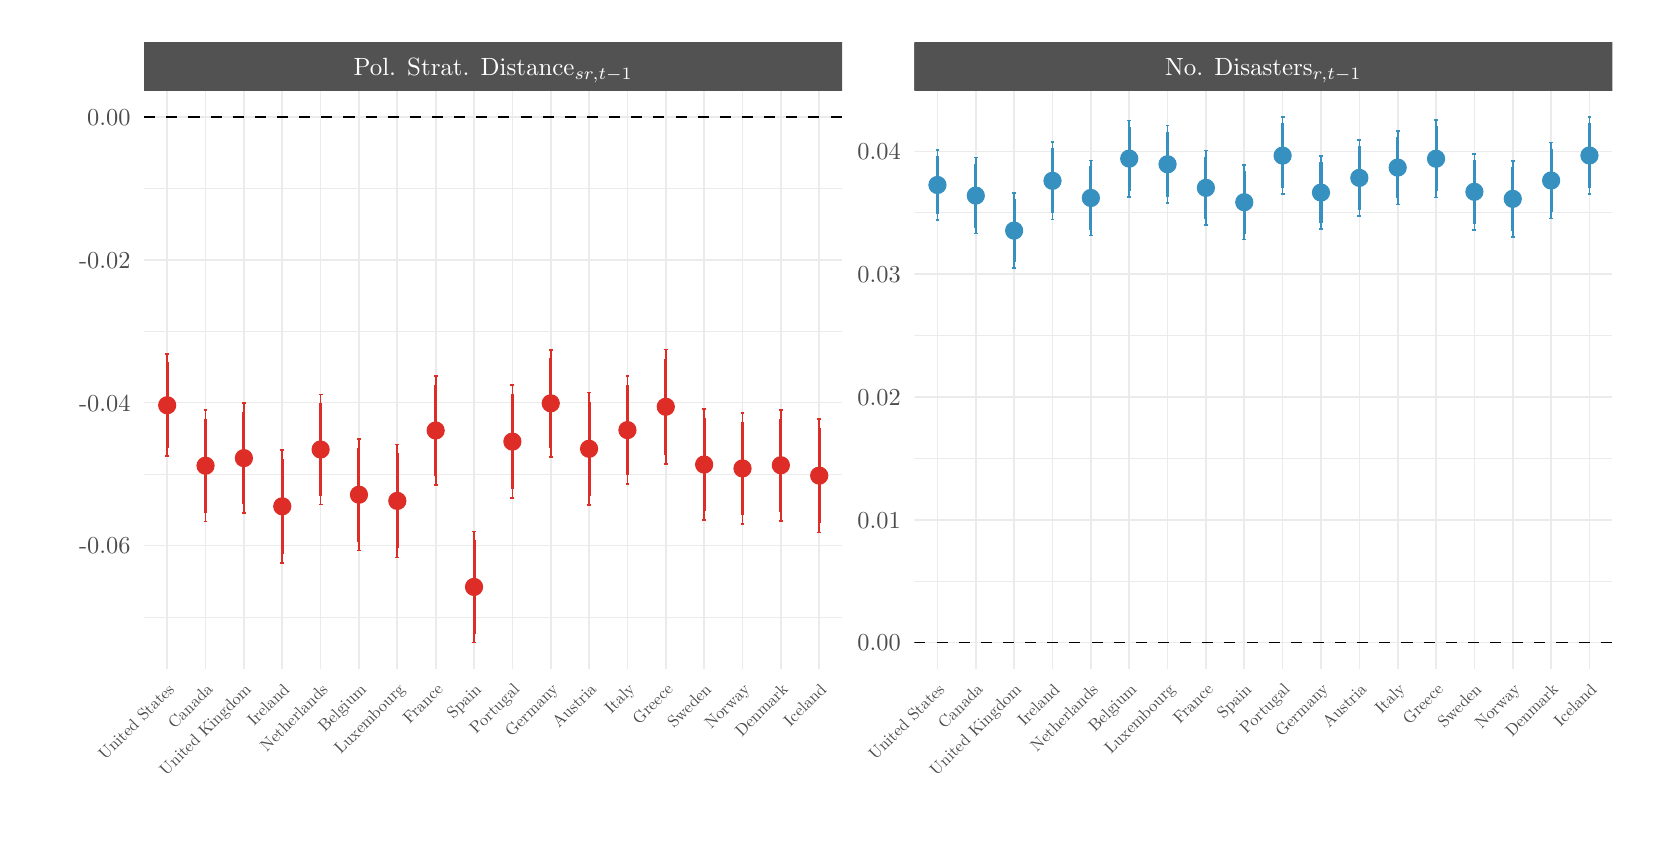
\begin{tikzpicture}[x=1pt,y=1pt]
\definecolor{fillColor}{RGB}{255,255,255}
\path[use as bounding box,fill=fillColor,fill opacity=0.00] (0,0) rectangle (578.16,289.08);
\begin{scope}
\path[clip] (  0.00,  0.00) rectangle (578.16,289.08);
\definecolor{drawColor}{RGB}{255,255,255}
\definecolor{fillColor}{RGB}{255,255,255}

\path[draw=drawColor,line width= 0.6pt,line join=round,line cap=round,fill=fillColor] (  0.00,  0.00) rectangle (578.16,289.08);
\end{scope}
\begin{scope}
\path[clip] ( 42.10, 57.44) rectangle (294.33,266.38);
\definecolor{fillColor}{RGB}{255,255,255}

\path[fill=fillColor] ( 42.10, 57.44) rectangle (294.33,266.38);
\definecolor{drawColor}{gray}{0.92}

\path[draw=drawColor,line width= 0.3pt,line join=round] ( 42.10, 76.10) --
	(294.33, 76.10);

\path[draw=drawColor,line width= 0.3pt,line join=round] ( 42.10,127.75) --
	(294.33,127.75);

\path[draw=drawColor,line width= 0.3pt,line join=round] ( 42.10,179.41) --
	(294.33,179.41);

\path[draw=drawColor,line width= 0.3pt,line join=round] ( 42.10,231.06) --
	(294.33,231.06);

\path[draw=drawColor,line width= 0.6pt,line join=round] ( 42.10,101.93) --
	(294.33,101.93);

\path[draw=drawColor,line width= 0.6pt,line join=round] ( 42.10,153.58) --
	(294.33,153.58);

\path[draw=drawColor,line width= 0.6pt,line join=round] ( 42.10,205.23) --
	(294.33,205.23);

\path[draw=drawColor,line width= 0.6pt,line join=round] ( 42.10,256.88) --
	(294.33,256.88);

\path[draw=drawColor,line width= 0.6pt,line join=round] ( 50.41, 57.44) --
	( 50.41,266.38);

\path[draw=drawColor,line width= 0.6pt,line join=round] ( 64.27, 57.44) --
	( 64.27,266.38);

\path[draw=drawColor,line width= 0.6pt,line join=round] ( 78.13, 57.44) --
	( 78.13,266.38);

\path[draw=drawColor,line width= 0.6pt,line join=round] ( 91.99, 57.44) --
	( 91.99,266.38);

\path[draw=drawColor,line width= 0.6pt,line join=round] (105.85, 57.44) --
	(105.85,266.38);

\path[draw=drawColor,line width= 0.6pt,line join=round] (119.71, 57.44) --
	(119.71,266.38);

\path[draw=drawColor,line width= 0.6pt,line join=round] (133.57, 57.44) --
	(133.57,266.38);

\path[draw=drawColor,line width= 0.6pt,line join=round] (147.43, 57.44) --
	(147.43,266.38);

\path[draw=drawColor,line width= 0.6pt,line join=round] (161.29, 57.44) --
	(161.29,266.38);

\path[draw=drawColor,line width= 0.6pt,line join=round] (175.15, 57.44) --
	(175.15,266.38);

\path[draw=drawColor,line width= 0.6pt,line join=round] (189.01, 57.44) --
	(189.01,266.38);

\path[draw=drawColor,line width= 0.6pt,line join=round] (202.86, 57.44) --
	(202.86,266.38);

\path[draw=drawColor,line width= 0.6pt,line join=round] (216.72, 57.44) --
	(216.72,266.38);

\path[draw=drawColor,line width= 0.6pt,line join=round] (230.58, 57.44) --
	(230.58,266.38);

\path[draw=drawColor,line width= 0.6pt,line join=round] (244.44, 57.44) --
	(244.44,266.38);

\path[draw=drawColor,line width= 0.6pt,line join=round] (258.30, 57.44) --
	(258.30,266.38);

\path[draw=drawColor,line width= 0.6pt,line join=round] (272.16, 57.44) --
	(272.16,266.38);

\path[draw=drawColor,line width= 0.6pt,line join=round] (286.02, 57.44) --
	(286.02,266.38);
\definecolor{drawColor}{RGB}{222,45,38}

\path[draw=drawColor,draw opacity=0.30,line width= 0.3pt,line join=round] ( 50.41,134.22) -- ( 50.41,171.07);

\path[draw=drawColor,draw opacity=0.30,line width= 0.3pt,line join=round] ( 64.27,110.59) -- ( 64.27,150.98);

\path[draw=drawColor,draw opacity=0.30,line width= 0.3pt,line join=round] ( 78.13,113.72) -- ( 78.13,153.36);

\path[draw=drawColor,draw opacity=0.30,line width= 0.3pt,line join=round] ( 91.99, 95.66) -- ( 91.99,136.58);

\path[draw=drawColor,draw opacity=0.30,line width= 0.3pt,line join=round] (105.85,116.78) -- (105.85,156.52);

\path[draw=drawColor,draw opacity=0.30,line width= 0.3pt,line join=round] (119.71,100.11) -- (119.71,140.51);

\path[draw=drawColor,draw opacity=0.30,line width= 0.3pt,line join=round] (133.57, 97.65) -- (133.57,138.51);

\path[draw=drawColor,draw opacity=0.30,line width= 0.3pt,line join=round] (147.43,123.78) -- (147.43,163.25);

\path[draw=drawColor,draw opacity=0.30,line width= 0.3pt,line join=round] (161.29, 66.93) -- (161.29,107.05);

\path[draw=drawColor,draw opacity=0.30,line width= 0.3pt,line join=round] (175.15,119.08) -- (175.15,159.93);

\path[draw=drawColor,draw opacity=0.30,line width= 0.3pt,line join=round] (189.01,133.97) -- (189.01,172.71);

\path[draw=drawColor,draw opacity=0.30,line width= 0.3pt,line join=round] (202.86,116.59) -- (202.86,157.24);

\path[draw=drawColor,draw opacity=0.30,line width= 0.3pt,line join=round] (216.72,124.23) -- (216.72,163.11);

\path[draw=drawColor,draw opacity=0.30,line width= 0.3pt,line join=round] (230.58,131.42) -- (230.58,172.76);

\path[draw=drawColor,draw opacity=0.30,line width= 0.3pt,line join=round] (244.44,111.13) -- (244.44,151.28);

\path[draw=drawColor,draw opacity=0.30,line width= 0.3pt,line join=round] (258.30,109.69) -- (258.30,149.94);

\path[draw=drawColor,draw opacity=0.30,line width= 0.3pt,line join=round] (272.16,110.90) -- (272.16,151.03);

\path[draw=drawColor,draw opacity=0.30,line width= 0.3pt,line join=round] (286.02,106.65) -- (286.02,147.77);
\definecolor{drawColor}{RGB}{222,45,38}

\path[draw=drawColor,line width= 1.1pt,line join=round] ( 50.41,137.18) -- ( 50.41,168.10);

\path[draw=drawColor,line width= 1.1pt,line join=round] ( 64.27,113.84) -- ( 64.27,147.74);

\path[draw=drawColor,line width= 1.1pt,line join=round] ( 78.13,116.91) -- ( 78.13,150.18);

\path[draw=drawColor,line width= 1.1pt,line join=round] ( 91.99, 98.95) -- ( 91.99,133.29);

\path[draw=drawColor,line width= 1.1pt,line join=round] (105.85,119.98) -- (105.85,153.32);

\path[draw=drawColor,line width= 1.1pt,line join=round] (119.71,103.36) -- (119.71,137.27);

\path[draw=drawColor,line width= 1.1pt,line join=round] (133.57,100.93) -- (133.57,135.22);

\path[draw=drawColor,line width= 1.1pt,line join=round] (147.43,126.95) -- (147.43,160.08);

\path[draw=drawColor,line width= 1.1pt,line join=round] (161.29, 70.16) -- (161.29,103.82);

\path[draw=drawColor,line width= 1.1pt,line join=round] (175.15,122.36) -- (175.15,156.65);

\path[draw=drawColor,line width= 1.1pt,line join=round] (189.01,137.09) -- (189.01,169.59);

\path[draw=drawColor,line width= 1.1pt,line join=round] (202.86,119.86) -- (202.86,153.97);

\path[draw=drawColor,line width= 1.1pt,line join=round] (216.72,127.36) -- (216.72,159.99);

\path[draw=drawColor,line width= 1.1pt,line join=round] (230.58,134.74) -- (230.58,169.43);

\path[draw=drawColor,line width= 1.1pt,line join=round] (244.44,114.36) -- (244.44,148.05);

\path[draw=drawColor,line width= 1.1pt,line join=round] (258.30,112.92) -- (258.30,146.70);

\path[draw=drawColor,line width= 1.1pt,line join=round] (272.16,114.12) -- (272.16,147.80);

\path[draw=drawColor,line width= 1.1pt,line join=round] (286.02,109.96) -- (286.02,144.47);
\definecolor{drawColor}{RGB}{0,0,0}

\path[draw=drawColor,line width= 0.6pt,dash pattern=on 4pt off 4pt ,line join=round] ( 42.10,256.88) -- (294.33,256.88);
\definecolor{drawColor}{RGB}{222,45,38}
\definecolor{fillColor}{RGB}{222,45,38}

\path[draw=drawColor,line width= 0.4pt,line join=round,line cap=round,fill=fillColor] ( 50.41,152.64) circle (  3.09);

\path[draw=drawColor,line width= 0.4pt,line join=round,line cap=round,fill=fillColor] ( 64.27,130.79) circle (  3.09);

\path[draw=drawColor,line width= 0.4pt,line join=round,line cap=round,fill=fillColor] ( 78.13,133.54) circle (  3.09);

\path[draw=drawColor,line width= 0.4pt,line join=round,line cap=round,fill=fillColor] ( 91.99,116.12) circle (  3.09);

\path[draw=drawColor,line width= 0.4pt,line join=round,line cap=round,fill=fillColor] (105.85,136.65) circle (  3.09);

\path[draw=drawColor,line width= 0.4pt,line join=round,line cap=round,fill=fillColor] (119.71,120.31) circle (  3.09);

\path[draw=drawColor,line width= 0.4pt,line join=round,line cap=round,fill=fillColor] (133.57,118.08) circle (  3.09);

\path[draw=drawColor,line width= 0.4pt,line join=round,line cap=round,fill=fillColor] (147.43,143.52) circle (  3.09);

\path[draw=drawColor,line width= 0.4pt,line join=round,line cap=round,fill=fillColor] (161.29, 86.99) circle (  3.09);

\path[draw=drawColor,line width= 0.4pt,line join=round,line cap=round,fill=fillColor] (175.15,139.51) circle (  3.09);

\path[draw=drawColor,line width= 0.4pt,line join=round,line cap=round,fill=fillColor] (189.01,153.34) circle (  3.09);

\path[draw=drawColor,line width= 0.4pt,line join=round,line cap=round,fill=fillColor] (202.86,136.91) circle (  3.09);

\path[draw=drawColor,line width= 0.4pt,line join=round,line cap=round,fill=fillColor] (216.72,143.67) circle (  3.09);

\path[draw=drawColor,line width= 0.4pt,line join=round,line cap=round,fill=fillColor] (230.58,152.09) circle (  3.09);

\path[draw=drawColor,line width= 0.4pt,line join=round,line cap=round,fill=fillColor] (244.44,131.21) circle (  3.09);

\path[draw=drawColor,line width= 0.4pt,line join=round,line cap=round,fill=fillColor] (258.30,129.81) circle (  3.09);

\path[draw=drawColor,line width= 0.4pt,line join=round,line cap=round,fill=fillColor] (272.16,130.96) circle (  3.09);

\path[draw=drawColor,line width= 0.4pt,line join=round,line cap=round,fill=fillColor] (286.02,127.21) circle (  3.09);

\path[draw=drawColor,line width= 0.6pt,line join=round] ( 49.72,171.07) --
	( 51.11,171.07);

\path[draw=drawColor,line width= 0.6pt,line join=round] ( 50.41,171.07) --
	( 50.41,134.22);

\path[draw=drawColor,line width= 0.6pt,line join=round] ( 49.72,134.22) --
	( 51.11,134.22);

\path[draw=drawColor,line width= 0.6pt,line join=round] ( 63.58,150.98) --
	( 64.97,150.98);

\path[draw=drawColor,line width= 0.6pt,line join=round] ( 64.27,150.98) --
	( 64.27,110.59);

\path[draw=drawColor,line width= 0.6pt,line join=round] ( 63.58,110.59) --
	( 64.97,110.59);

\path[draw=drawColor,line width= 0.6pt,line join=round] ( 77.44,153.36) --
	( 78.83,153.36);

\path[draw=drawColor,line width= 0.6pt,line join=round] ( 78.13,153.36) --
	( 78.13,113.72);

\path[draw=drawColor,line width= 0.6pt,line join=round] ( 77.44,113.72) --
	( 78.83,113.72);

\path[draw=drawColor,line width= 0.6pt,line join=round] ( 91.30,136.58) --
	( 92.68,136.58);

\path[draw=drawColor,line width= 0.6pt,line join=round] ( 91.99,136.58) --
	( 91.99, 95.66);

\path[draw=drawColor,line width= 0.6pt,line join=round] ( 91.30, 95.66) --
	( 92.68, 95.66);

\path[draw=drawColor,line width= 0.6pt,line join=round] (105.16,156.52) --
	(106.54,156.52);

\path[draw=drawColor,line width= 0.6pt,line join=round] (105.85,156.52) --
	(105.85,116.78);

\path[draw=drawColor,line width= 0.6pt,line join=round] (105.16,116.78) --
	(106.54,116.78);

\path[draw=drawColor,line width= 0.6pt,line join=round] (119.02,140.51) --
	(120.40,140.51);

\path[draw=drawColor,line width= 0.6pt,line join=round] (119.71,140.51) --
	(119.71,100.11);

\path[draw=drawColor,line width= 0.6pt,line join=round] (119.02,100.11) --
	(120.40,100.11);

\path[draw=drawColor,line width= 0.6pt,line join=round] (132.88,138.51) --
	(134.26,138.51);

\path[draw=drawColor,line width= 0.6pt,line join=round] (133.57,138.51) --
	(133.57, 97.65);

\path[draw=drawColor,line width= 0.6pt,line join=round] (132.88, 97.65) --
	(134.26, 97.65);

\path[draw=drawColor,line width= 0.6pt,line join=round] (146.74,163.25) --
	(148.12,163.25);

\path[draw=drawColor,line width= 0.6pt,line join=round] (147.43,163.25) --
	(147.43,123.78);

\path[draw=drawColor,line width= 0.6pt,line join=round] (146.74,123.78) --
	(148.12,123.78);

\path[draw=drawColor,line width= 0.6pt,line join=round] (160.59,107.05) --
	(161.98,107.05);

\path[draw=drawColor,line width= 0.6pt,line join=round] (161.29,107.05) --
	(161.29, 66.93);

\path[draw=drawColor,line width= 0.6pt,line join=round] (160.59, 66.93) --
	(161.98, 66.93);

\path[draw=drawColor,line width= 0.6pt,line join=round] (174.45,159.93) --
	(175.84,159.93);

\path[draw=drawColor,line width= 0.6pt,line join=round] (175.15,159.93) --
	(175.15,119.08);

\path[draw=drawColor,line width= 0.6pt,line join=round] (174.45,119.08) --
	(175.84,119.08);

\path[draw=drawColor,line width= 0.6pt,line join=round] (188.31,172.71) --
	(189.70,172.71);

\path[draw=drawColor,line width= 0.6pt,line join=round] (189.01,172.71) --
	(189.01,133.97);

\path[draw=drawColor,line width= 0.6pt,line join=round] (188.31,133.97) --
	(189.70,133.97);

\path[draw=drawColor,line width= 0.6pt,line join=round] (202.17,157.24) --
	(203.56,157.24);

\path[draw=drawColor,line width= 0.6pt,line join=round] (202.86,157.24) --
	(202.86,116.59);

\path[draw=drawColor,line width= 0.6pt,line join=round] (202.17,116.59) --
	(203.56,116.59);

\path[draw=drawColor,line width= 0.6pt,line join=round] (216.03,163.11) --
	(217.42,163.11);

\path[draw=drawColor,line width= 0.6pt,line join=round] (216.72,163.11) --
	(216.72,124.23);

\path[draw=drawColor,line width= 0.6pt,line join=round] (216.03,124.23) --
	(217.42,124.23);

\path[draw=drawColor,line width= 0.6pt,line join=round] (229.89,172.76) --
	(231.28,172.76);

\path[draw=drawColor,line width= 0.6pt,line join=round] (230.58,172.76) --
	(230.58,131.42);

\path[draw=drawColor,line width= 0.6pt,line join=round] (229.89,131.42) --
	(231.28,131.42);

\path[draw=drawColor,line width= 0.6pt,line join=round] (243.75,151.28) --
	(245.13,151.28);

\path[draw=drawColor,line width= 0.6pt,line join=round] (244.44,151.28) --
	(244.44,111.13);

\path[draw=drawColor,line width= 0.6pt,line join=round] (243.75,111.13) --
	(245.13,111.13);

\path[draw=drawColor,line width= 0.6pt,line join=round] (257.61,149.94) --
	(258.99,149.94);

\path[draw=drawColor,line width= 0.6pt,line join=round] (258.30,149.94) --
	(258.30,109.69);

\path[draw=drawColor,line width= 0.6pt,line join=round] (257.61,109.69) --
	(258.99,109.69);

\path[draw=drawColor,line width= 0.6pt,line join=round] (271.47,151.03) --
	(272.85,151.03);

\path[draw=drawColor,line width= 0.6pt,line join=round] (272.16,151.03) --
	(272.16,110.90);

\path[draw=drawColor,line width= 0.6pt,line join=round] (271.47,110.90) --
	(272.85,110.90);

\path[draw=drawColor,line width= 0.6pt,line join=round] (285.33,147.77) --
	(286.71,147.77);

\path[draw=drawColor,line width= 0.6pt,line join=round] (286.02,147.77) --
	(286.02,106.65);

\path[draw=drawColor,line width= 0.6pt,line join=round] (285.33,106.65) --
	(286.71,106.65);
\end{scope}
\begin{scope}
\path[clip] (320.42, 57.44) rectangle (572.66,266.38);
\definecolor{fillColor}{RGB}{255,255,255}

\path[fill=fillColor] (320.42, 57.44) rectangle (572.66,266.38);
\definecolor{drawColor}{gray}{0.92}

\path[draw=drawColor,line width= 0.3pt,line join=round] (320.42, 89.11) --
	(572.66, 89.11);

\path[draw=drawColor,line width= 0.3pt,line join=round] (320.42,133.47) --
	(572.66,133.47);

\path[draw=drawColor,line width= 0.3pt,line join=round] (320.42,177.82) --
	(572.66,177.82);

\path[draw=drawColor,line width= 0.3pt,line join=round] (320.42,222.18) --
	(572.66,222.18);

\path[draw=drawColor,line width= 0.6pt,line join=round] (320.42, 66.93) --
	(572.66, 66.93);

\path[draw=drawColor,line width= 0.6pt,line join=round] (320.42,111.29) --
	(572.66,111.29);

\path[draw=drawColor,line width= 0.6pt,line join=round] (320.42,155.64) --
	(572.66,155.64);

\path[draw=drawColor,line width= 0.6pt,line join=round] (320.42,200.00) --
	(572.66,200.00);

\path[draw=drawColor,line width= 0.6pt,line join=round] (320.42,244.35) --
	(572.66,244.35);

\path[draw=drawColor,line width= 0.6pt,line join=round] (328.74, 57.44) --
	(328.74,266.38);

\path[draw=drawColor,line width= 0.6pt,line join=round] (342.60, 57.44) --
	(342.60,266.38);

\path[draw=drawColor,line width= 0.6pt,line join=round] (356.46, 57.44) --
	(356.46,266.38);

\path[draw=drawColor,line width= 0.6pt,line join=round] (370.32, 57.44) --
	(370.32,266.38);

\path[draw=drawColor,line width= 0.6pt,line join=round] (384.18, 57.44) --
	(384.18,266.38);

\path[draw=drawColor,line width= 0.6pt,line join=round] (398.04, 57.44) --
	(398.04,266.38);

\path[draw=drawColor,line width= 0.6pt,line join=round] (411.89, 57.44) --
	(411.89,266.38);

\path[draw=drawColor,line width= 0.6pt,line join=round] (425.75, 57.44) --
	(425.75,266.38);

\path[draw=drawColor,line width= 0.6pt,line join=round] (439.61, 57.44) --
	(439.61,266.38);

\path[draw=drawColor,line width= 0.6pt,line join=round] (453.47, 57.44) --
	(453.47,266.38);

\path[draw=drawColor,line width= 0.6pt,line join=round] (467.33, 57.44) --
	(467.33,266.38);

\path[draw=drawColor,line width= 0.6pt,line join=round] (481.19, 57.44) --
	(481.19,266.38);

\path[draw=drawColor,line width= 0.6pt,line join=round] (495.05, 57.44) --
	(495.05,266.38);

\path[draw=drawColor,line width= 0.6pt,line join=round] (508.91, 57.44) --
	(508.91,266.38);

\path[draw=drawColor,line width= 0.6pt,line join=round] (522.77, 57.44) --
	(522.77,266.38);

\path[draw=drawColor,line width= 0.6pt,line join=round] (536.63, 57.44) --
	(536.63,266.38);

\path[draw=drawColor,line width= 0.6pt,line join=round] (550.49, 57.44) --
	(550.49,266.38);

\path[draw=drawColor,line width= 0.6pt,line join=round] (564.34, 57.44) --
	(564.34,266.38);
\definecolor{drawColor}{RGB}{54,144,192}

\path[draw=drawColor,draw opacity=0.30,line width= 0.3pt,line join=round] (328.74,219.59) -- (328.74,244.87);

\path[draw=drawColor,draw opacity=0.30,line width= 0.3pt,line join=round] (342.60,214.65) -- (342.60,242.12);

\path[draw=drawColor,draw opacity=0.30,line width= 0.3pt,line join=round] (356.46,202.18) -- (356.46,229.30);

\path[draw=drawColor,draw opacity=0.30,line width= 0.3pt,line join=round] (370.32,219.80) -- (370.32,247.68);

\path[draw=drawColor,draw opacity=0.30,line width= 0.3pt,line join=round] (384.18,213.94) -- (384.18,241.13);

\path[draw=drawColor,draw opacity=0.30,line width= 0.3pt,line join=round] (398.04,227.94) -- (398.04,255.57);

\path[draw=drawColor,draw opacity=0.30,line width= 0.3pt,line join=round] (411.89,225.75) -- (411.89,253.67);

\path[draw=drawColor,draw opacity=0.30,line width= 0.3pt,line join=round] (425.75,217.70) -- (425.75,244.69);

\path[draw=drawColor,draw opacity=0.30,line width= 0.3pt,line join=round] (439.61,212.48) -- (439.61,239.53);

\path[draw=drawColor,draw opacity=0.30,line width= 0.3pt,line join=round] (453.47,228.94) -- (453.47,256.76);

\path[draw=drawColor,draw opacity=0.30,line width= 0.3pt,line join=round] (467.33,216.23) -- (467.33,242.76);

\path[draw=drawColor,draw opacity=0.30,line width= 0.3pt,line join=round] (481.19,221.01) -- (481.19,248.59);

\path[draw=drawColor,draw opacity=0.30,line width= 0.3pt,line join=round] (495.05,225.21) -- (495.05,251.82);

\path[draw=drawColor,draw opacity=0.30,line width= 0.3pt,line join=round] (508.91,227.76) -- (508.91,255.69);

\path[draw=drawColor,draw opacity=0.30,line width= 0.3pt,line join=round] (522.77,216.08) -- (522.77,243.47);

\path[draw=drawColor,draw opacity=0.30,line width= 0.3pt,line join=round] (536.63,213.49) -- (536.63,240.95);

\path[draw=drawColor,draw opacity=0.30,line width= 0.3pt,line join=round] (550.49,220.13) -- (550.49,247.57);

\path[draw=drawColor,draw opacity=0.30,line width= 0.3pt,line join=round] (564.34,228.90) -- (564.34,256.88);
\definecolor{drawColor}{RGB}{54,144,192}

\path[draw=drawColor,line width= 1.1pt,line join=round] (328.74,221.62) -- (328.74,242.84);

\path[draw=drawColor,line width= 1.1pt,line join=round] (342.60,216.86) -- (342.60,239.91);

\path[draw=drawColor,line width= 1.1pt,line join=round] (356.46,204.36) -- (356.46,227.12);

\path[draw=drawColor,line width= 1.1pt,line join=round] (370.32,222.04) -- (370.32,245.44);

\path[draw=drawColor,line width= 1.1pt,line join=round] (384.18,216.12) -- (384.18,238.95);

\path[draw=drawColor,line width= 1.1pt,line join=round] (398.04,230.16) -- (398.04,253.35);

\path[draw=drawColor,line width= 1.1pt,line join=round] (411.89,227.99) -- (411.89,251.42);

\path[draw=drawColor,line width= 1.1pt,line join=round] (425.75,219.87) -- (425.75,242.52);

\path[draw=drawColor,line width= 1.1pt,line join=round] (439.61,214.65) -- (439.61,237.36);

\path[draw=drawColor,line width= 1.1pt,line join=round] (453.47,231.17) -- (453.47,254.52);

\path[draw=drawColor,line width= 1.1pt,line join=round] (467.33,218.36) -- (467.33,240.62);

\path[draw=drawColor,line width= 1.1pt,line join=round] (481.19,223.23) -- (481.19,246.38);

\path[draw=drawColor,line width= 1.1pt,line join=round] (495.05,227.35) -- (495.05,249.68);

\path[draw=drawColor,line width= 1.1pt,line join=round] (508.91,230.00) -- (508.91,253.44);

\path[draw=drawColor,line width= 1.1pt,line join=round] (522.77,218.28) -- (522.77,241.27);

\path[draw=drawColor,line width= 1.1pt,line join=round] (536.63,215.70) -- (536.63,238.74);

\path[draw=drawColor,line width= 1.1pt,line join=round] (550.49,222.34) -- (550.49,245.36);

\path[draw=drawColor,line width= 1.1pt,line join=round] (564.34,231.15) -- (564.34,254.63);
\definecolor{drawColor}{RGB}{0,0,0}

\path[draw=drawColor,line width= 0.6pt,dash pattern=on 4pt off 4pt ,line join=round] (320.42, 66.93) -- (572.66, 66.93);
\definecolor{drawColor}{RGB}{54,144,192}
\definecolor{fillColor}{RGB}{54,144,192}

\path[draw=drawColor,line width= 0.4pt,line join=round,line cap=round,fill=fillColor] (328.74,232.23) circle (  3.09);

\path[draw=drawColor,line width= 0.4pt,line join=round,line cap=round,fill=fillColor] (342.60,228.39) circle (  3.09);

\path[draw=drawColor,line width= 0.4pt,line join=round,line cap=round,fill=fillColor] (356.46,215.74) circle (  3.09);

\path[draw=drawColor,line width= 0.4pt,line join=round,line cap=round,fill=fillColor] (370.32,233.74) circle (  3.09);

\path[draw=drawColor,line width= 0.4pt,line join=round,line cap=round,fill=fillColor] (384.18,227.54) circle (  3.09);

\path[draw=drawColor,line width= 0.4pt,line join=round,line cap=round,fill=fillColor] (398.04,241.76) circle (  3.09);

\path[draw=drawColor,line width= 0.4pt,line join=round,line cap=round,fill=fillColor] (411.89,239.71) circle (  3.09);

\path[draw=drawColor,line width= 0.4pt,line join=round,line cap=round,fill=fillColor] (425.75,231.19) circle (  3.09);

\path[draw=drawColor,line width= 0.4pt,line join=round,line cap=round,fill=fillColor] (439.61,226.00) circle (  3.09);

\path[draw=drawColor,line width= 0.4pt,line join=round,line cap=round,fill=fillColor] (453.47,242.85) circle (  3.09);

\path[draw=drawColor,line width= 0.4pt,line join=round,line cap=round,fill=fillColor] (467.33,229.49) circle (  3.09);

\path[draw=drawColor,line width= 0.4pt,line join=round,line cap=round,fill=fillColor] (481.19,234.80) circle (  3.09);

\path[draw=drawColor,line width= 0.4pt,line join=round,line cap=round,fill=fillColor] (495.05,238.52) circle (  3.09);

\path[draw=drawColor,line width= 0.4pt,line join=round,line cap=round,fill=fillColor] (508.91,241.72) circle (  3.09);

\path[draw=drawColor,line width= 0.4pt,line join=round,line cap=round,fill=fillColor] (522.77,229.77) circle (  3.09);

\path[draw=drawColor,line width= 0.4pt,line join=round,line cap=round,fill=fillColor] (536.63,227.22) circle (  3.09);

\path[draw=drawColor,line width= 0.4pt,line join=round,line cap=round,fill=fillColor] (550.49,233.85) circle (  3.09);

\path[draw=drawColor,line width= 0.4pt,line join=round,line cap=round,fill=fillColor] (564.34,242.89) circle (  3.09);

\path[draw=drawColor,line width= 0.6pt,line join=round] (328.05,244.87) --
	(329.43,244.87);

\path[draw=drawColor,line width= 0.6pt,line join=round] (328.74,244.87) --
	(328.74,219.59);

\path[draw=drawColor,line width= 0.6pt,line join=round] (328.05,219.59) --
	(329.43,219.59);

\path[draw=drawColor,line width= 0.6pt,line join=round] (341.91,242.12) --
	(343.29,242.12);

\path[draw=drawColor,line width= 0.6pt,line join=round] (342.60,242.12) --
	(342.60,214.65);

\path[draw=drawColor,line width= 0.6pt,line join=round] (341.91,214.65) --
	(343.29,214.65);

\path[draw=drawColor,line width= 0.6pt,line join=round] (355.77,229.30) --
	(357.15,229.30);

\path[draw=drawColor,line width= 0.6pt,line join=round] (356.46,229.30) --
	(356.46,202.18);

\path[draw=drawColor,line width= 0.6pt,line join=round] (355.77,202.18) --
	(357.15,202.18);

\path[draw=drawColor,line width= 0.6pt,line join=round] (369.62,247.68) --
	(371.01,247.68);

\path[draw=drawColor,line width= 0.6pt,line join=round] (370.32,247.68) --
	(370.32,219.80);

\path[draw=drawColor,line width= 0.6pt,line join=round] (369.62,219.80) --
	(371.01,219.80);

\path[draw=drawColor,line width= 0.6pt,line join=round] (383.48,241.13) --
	(384.87,241.13);

\path[draw=drawColor,line width= 0.6pt,line join=round] (384.18,241.13) --
	(384.18,213.94);

\path[draw=drawColor,line width= 0.6pt,line join=round] (383.48,213.94) --
	(384.87,213.94);

\path[draw=drawColor,line width= 0.6pt,line join=round] (397.34,255.57) --
	(398.73,255.57);

\path[draw=drawColor,line width= 0.6pt,line join=round] (398.04,255.57) --
	(398.04,227.94);

\path[draw=drawColor,line width= 0.6pt,line join=round] (397.34,227.94) --
	(398.73,227.94);

\path[draw=drawColor,line width= 0.6pt,line join=round] (411.20,253.67) --
	(412.59,253.67);

\path[draw=drawColor,line width= 0.6pt,line join=round] (411.89,253.67) --
	(411.89,225.75);

\path[draw=drawColor,line width= 0.6pt,line join=round] (411.20,225.75) --
	(412.59,225.75);

\path[draw=drawColor,line width= 0.6pt,line join=round] (425.06,244.69) --
	(426.45,244.69);

\path[draw=drawColor,line width= 0.6pt,line join=round] (425.75,244.69) --
	(425.75,217.70);

\path[draw=drawColor,line width= 0.6pt,line join=round] (425.06,217.70) --
	(426.45,217.70);

\path[draw=drawColor,line width= 0.6pt,line join=round] (438.92,239.53) --
	(440.31,239.53);

\path[draw=drawColor,line width= 0.6pt,line join=round] (439.61,239.53) --
	(439.61,212.48);

\path[draw=drawColor,line width= 0.6pt,line join=round] (438.92,212.48) --
	(440.31,212.48);

\path[draw=drawColor,line width= 0.6pt,line join=round] (452.78,256.76) --
	(454.16,256.76);

\path[draw=drawColor,line width= 0.6pt,line join=round] (453.47,256.76) --
	(453.47,228.94);

\path[draw=drawColor,line width= 0.6pt,line join=round] (452.78,228.94) --
	(454.16,228.94);

\path[draw=drawColor,line width= 0.6pt,line join=round] (466.64,242.76) --
	(468.02,242.76);

\path[draw=drawColor,line width= 0.6pt,line join=round] (467.33,242.76) --
	(467.33,216.23);

\path[draw=drawColor,line width= 0.6pt,line join=round] (466.64,216.23) --
	(468.02,216.23);

\path[draw=drawColor,line width= 0.6pt,line join=round] (480.50,248.59) --
	(481.88,248.59);

\path[draw=drawColor,line width= 0.6pt,line join=round] (481.19,248.59) --
	(481.19,221.01);

\path[draw=drawColor,line width= 0.6pt,line join=round] (480.50,221.01) --
	(481.88,221.01);

\path[draw=drawColor,line width= 0.6pt,line join=round] (494.36,251.82) --
	(495.74,251.82);

\path[draw=drawColor,line width= 0.6pt,line join=round] (495.05,251.82) --
	(495.05,225.21);

\path[draw=drawColor,line width= 0.6pt,line join=round] (494.36,225.21) --
	(495.74,225.21);

\path[draw=drawColor,line width= 0.6pt,line join=round] (508.22,255.69) --
	(509.60,255.69);

\path[draw=drawColor,line width= 0.6pt,line join=round] (508.91,255.69) --
	(508.91,227.76);

\path[draw=drawColor,line width= 0.6pt,line join=round] (508.22,227.76) --
	(509.60,227.76);

\path[draw=drawColor,line width= 0.6pt,line join=round] (522.07,243.47) --
	(523.46,243.47);

\path[draw=drawColor,line width= 0.6pt,line join=round] (522.77,243.47) --
	(522.77,216.08);

\path[draw=drawColor,line width= 0.6pt,line join=round] (522.07,216.08) --
	(523.46,216.08);

\path[draw=drawColor,line width= 0.6pt,line join=round] (535.93,240.95) --
	(537.32,240.95);

\path[draw=drawColor,line width= 0.6pt,line join=round] (536.63,240.95) --
	(536.63,213.49);

\path[draw=drawColor,line width= 0.6pt,line join=round] (535.93,213.49) --
	(537.32,213.49);

\path[draw=drawColor,line width= 0.6pt,line join=round] (549.79,247.57) --
	(551.18,247.57);

\path[draw=drawColor,line width= 0.6pt,line join=round] (550.49,247.57) --
	(550.49,220.13);

\path[draw=drawColor,line width= 0.6pt,line join=round] (549.79,220.13) --
	(551.18,220.13);

\path[draw=drawColor,line width= 0.6pt,line join=round] (563.65,256.88) --
	(565.04,256.88);

\path[draw=drawColor,line width= 0.6pt,line join=round] (564.34,256.88) --
	(564.34,228.90);

\path[draw=drawColor,line width= 0.6pt,line join=round] (563.65,228.90) --
	(565.04,228.90);
\end{scope}
\begin{scope}
\path[clip] ( 42.10,266.38) rectangle (294.33,283.58);
\definecolor{drawColor}{gray}{0.32}
\definecolor{fillColor}{gray}{0.32}

\path[draw=drawColor,line width= 0.6pt,line join=round,line cap=round,fill=fillColor] ( 42.10,266.38) rectangle (294.33,283.58);
\definecolor{drawColor}{RGB}{255,255,255}

\node[text=drawColor,anchor=base,inner sep=0pt, outer sep=0pt, scale=  0.90] at (168.22,271.88) {Pol. Strat. Distance$_{sr,t-1}$};
\end{scope}
\begin{scope}
\path[clip] (320.42,266.38) rectangle (572.66,283.58);
\definecolor{drawColor}{gray}{0.32}
\definecolor{fillColor}{gray}{0.32}

\path[draw=drawColor,line width= 0.6pt,line join=round,line cap=round,fill=fillColor] (320.42,266.38) rectangle (572.66,283.58);
\definecolor{drawColor}{RGB}{255,255,255}

\node[text=drawColor,anchor=base,inner sep=0pt, outer sep=0pt, scale=  0.90] at (446.54,271.88) {No. Disasters$_{r,t-1}$};
\end{scope}
\begin{scope}
\path[clip] (  0.00,  0.00) rectangle (578.16,289.08);
\definecolor{drawColor}{gray}{0.30}

\node[text=drawColor,rotate= 45.00,anchor=base east,inner sep=0pt, outer sep=0pt, scale=  0.60] at ( 53.34, 49.56) {United States};

\node[text=drawColor,rotate= 45.00,anchor=base east,inner sep=0pt, outer sep=0pt, scale=  0.60] at ( 67.20, 49.56) {Canada};

\node[text=drawColor,rotate= 45.00,anchor=base east,inner sep=0pt, outer sep=0pt, scale=  0.60] at ( 81.05, 49.56) {United Kingdom};

\node[text=drawColor,rotate= 45.00,anchor=base east,inner sep=0pt, outer sep=0pt, scale=  0.60] at ( 94.91, 49.56) {Ireland};

\node[text=drawColor,rotate= 45.00,anchor=base east,inner sep=0pt, outer sep=0pt, scale=  0.60] at (108.77, 49.56) {Netherlands};

\node[text=drawColor,rotate= 45.00,anchor=base east,inner sep=0pt, outer sep=0pt, scale=  0.60] at (122.63, 49.56) {Belgium};

\node[text=drawColor,rotate= 45.00,anchor=base east,inner sep=0pt, outer sep=0pt, scale=  0.60] at (136.49, 49.56) {Luxembourg};

\node[text=drawColor,rotate= 45.00,anchor=base east,inner sep=0pt, outer sep=0pt, scale=  0.60] at (150.35, 49.56) {France};

\node[text=drawColor,rotate= 45.00,anchor=base east,inner sep=0pt, outer sep=0pt, scale=  0.60] at (164.21, 49.56) {Spain};

\node[text=drawColor,rotate= 45.00,anchor=base east,inner sep=0pt, outer sep=0pt, scale=  0.60] at (178.07, 49.56) {Portugal};

\node[text=drawColor,rotate= 45.00,anchor=base east,inner sep=0pt, outer sep=0pt, scale=  0.60] at (191.93, 49.56) {Germany};

\node[text=drawColor,rotate= 45.00,anchor=base east,inner sep=0pt, outer sep=0pt, scale=  0.60] at (205.79, 49.56) {Austria};

\node[text=drawColor,rotate= 45.00,anchor=base east,inner sep=0pt, outer sep=0pt, scale=  0.60] at (219.65, 49.56) {Italy};

\node[text=drawColor,rotate= 45.00,anchor=base east,inner sep=0pt, outer sep=0pt, scale=  0.60] at (233.50, 49.56) {Greece};

\node[text=drawColor,rotate= 45.00,anchor=base east,inner sep=0pt, outer sep=0pt, scale=  0.60] at (247.36, 49.56) {Sweden};

\node[text=drawColor,rotate= 45.00,anchor=base east,inner sep=0pt, outer sep=0pt, scale=  0.60] at (261.22, 49.56) {Norway};

\node[text=drawColor,rotate= 45.00,anchor=base east,inner sep=0pt, outer sep=0pt, scale=  0.60] at (275.08, 49.56) {Denmark};

\node[text=drawColor,rotate= 45.00,anchor=base east,inner sep=0pt, outer sep=0pt, scale=  0.60] at (288.94, 49.56) {Iceland};
\end{scope}
\begin{scope}
\path[clip] (  0.00,  0.00) rectangle (578.16,289.08);
\definecolor{drawColor}{gray}{0.30}

\node[text=drawColor,rotate= 45.00,anchor=base east,inner sep=0pt, outer sep=0pt, scale=  0.60] at (331.66, 49.56) {United States};

\node[text=drawColor,rotate= 45.00,anchor=base east,inner sep=0pt, outer sep=0pt, scale=  0.60] at (345.52, 49.56) {Canada};

\node[text=drawColor,rotate= 45.00,anchor=base east,inner sep=0pt, outer sep=0pt, scale=  0.60] at (359.38, 49.56) {United Kingdom};

\node[text=drawColor,rotate= 45.00,anchor=base east,inner sep=0pt, outer sep=0pt, scale=  0.60] at (373.24, 49.56) {Ireland};

\node[text=drawColor,rotate= 45.00,anchor=base east,inner sep=0pt, outer sep=0pt, scale=  0.60] at (387.10, 49.56) {Netherlands};

\node[text=drawColor,rotate= 45.00,anchor=base east,inner sep=0pt, outer sep=0pt, scale=  0.60] at (400.96, 49.56) {Belgium};

\node[text=drawColor,rotate= 45.00,anchor=base east,inner sep=0pt, outer sep=0pt, scale=  0.60] at (414.82, 49.56) {Luxembourg};

\node[text=drawColor,rotate= 45.00,anchor=base east,inner sep=0pt, outer sep=0pt, scale=  0.60] at (428.68, 49.56) {France};

\node[text=drawColor,rotate= 45.00,anchor=base east,inner sep=0pt, outer sep=0pt, scale=  0.60] at (442.53, 49.56) {Spain};

\node[text=drawColor,rotate= 45.00,anchor=base east,inner sep=0pt, outer sep=0pt, scale=  0.60] at (456.39, 49.56) {Portugal};

\node[text=drawColor,rotate= 45.00,anchor=base east,inner sep=0pt, outer sep=0pt, scale=  0.60] at (470.25, 49.56) {Germany};

\node[text=drawColor,rotate= 45.00,anchor=base east,inner sep=0pt, outer sep=0pt, scale=  0.60] at (484.11, 49.56) {Austria};

\node[text=drawColor,rotate= 45.00,anchor=base east,inner sep=0pt, outer sep=0pt, scale=  0.60] at (497.97, 49.56) {Italy};

\node[text=drawColor,rotate= 45.00,anchor=base east,inner sep=0pt, outer sep=0pt, scale=  0.60] at (511.83, 49.56) {Greece};

\node[text=drawColor,rotate= 45.00,anchor=base east,inner sep=0pt, outer sep=0pt, scale=  0.60] at (525.69, 49.56) {Sweden};

\node[text=drawColor,rotate= 45.00,anchor=base east,inner sep=0pt, outer sep=0pt, scale=  0.60] at (539.55, 49.56) {Norway};

\node[text=drawColor,rotate= 45.00,anchor=base east,inner sep=0pt, outer sep=0pt, scale=  0.60] at (553.41, 49.56) {Denmark};

\node[text=drawColor,rotate= 45.00,anchor=base east,inner sep=0pt, outer sep=0pt, scale=  0.60] at (567.27, 49.56) {Iceland};
\end{scope}
\begin{scope}
\path[clip] (  0.00,  0.00) rectangle (578.16,289.08);
\definecolor{drawColor}{gray}{0.30}

\node[text=drawColor,anchor=base east,inner sep=0pt, outer sep=0pt, scale=  0.88] at (315.47, 63.90) {0.00};

\node[text=drawColor,anchor=base east,inner sep=0pt, outer sep=0pt, scale=  0.88] at (315.47,108.26) {0.01};

\node[text=drawColor,anchor=base east,inner sep=0pt, outer sep=0pt, scale=  0.88] at (315.47,152.61) {0.02};

\node[text=drawColor,anchor=base east,inner sep=0pt, outer sep=0pt, scale=  0.88] at (315.47,196.97) {0.03};

\node[text=drawColor,anchor=base east,inner sep=0pt, outer sep=0pt, scale=  0.88] at (315.47,241.32) {0.04};
\end{scope}
\begin{scope}
\path[clip] (  0.00,  0.00) rectangle (578.16,289.08);
\definecolor{drawColor}{gray}{0.30}

\node[text=drawColor,anchor=base east,inner sep=0pt, outer sep=0pt, scale=  0.88] at ( 37.15, 98.90) {-0.06};

\node[text=drawColor,anchor=base east,inner sep=0pt, outer sep=0pt, scale=  0.88] at ( 37.15,150.55) {-0.04};

\node[text=drawColor,anchor=base east,inner sep=0pt, outer sep=0pt, scale=  0.88] at ( 37.15,202.20) {-0.02};

\node[text=drawColor,anchor=base east,inner sep=0pt, outer sep=0pt, scale=  0.88] at ( 37.15,253.85) {0.00};
\end{scope}
\end{tikzpicture}
}
} 
%%%%%%%%%%%%%%%%%%%%%%%%%%%%%%%%%%%%%%%%%%%%%%%%%%%%%%%%%%%%

%%%%%%%%%%%%%%%%%%%%%%%%%%%%%%%%%%%%%%%%%%%%%%%%%%%%%%%%%%%%
\frame
{
  \frametitle{benefits of latent space approach}
    \centering
  \resizebox{1\textwidth}{!}{% Created by tikzDevice version 0.8.1 on 2015-03-26 22:10:23
% !TEX encoding = UTF-8 Unicode
\begin{tikzpicture}[x=1pt,y=1pt]
\definecolor{fillColor}{RGB}{255,255,255}
\path[use as bounding box,fill=fillColor,fill opacity=0.00] (0,0) rectangle (578.16,361.35);
\begin{scope}
\path[clip] (  0.00,  0.00) rectangle (578.16,361.35);
\definecolor{drawColor}{RGB}{255,255,255}
\definecolor{fillColor}{RGB}{255,255,255}

\path[draw=drawColor,line width= 0.6pt,line join=round,line cap=round,fill=fillColor] (  0.00,  0.00) rectangle (578.16,361.35);
\end{scope}
\begin{scope}
\path[clip] ( 92.81, 34.03) rectangle (566.12,349.30);
\definecolor{fillColor}{RGB}{255,255,255}

\path[fill=fillColor] ( 92.81, 34.03) rectangle (566.12,349.30);
\definecolor{fillColor}{RGB}{0,0,0}

\path[fill=fillColor] (133.42,312.93) circle (  2.13);

\path[fill=fillColor] (500.77,252.30) circle (  2.13);

\path[fill=fillColor] (480.65,191.67) circle (  2.13);

\path[fill=fillColor] (459.02,131.04) circle (  2.13);

\path[fill=fillColor] (366.97, 70.41) circle (  2.13);
\definecolor{drawColor}{RGB}{0,0,0}

\path[draw=drawColor,line width= 0.6pt,line join=round] (336.72, 70.41) -- (398.57, 70.41);

\path[draw=drawColor,line width= 0.6pt,line join=round] (432.48,131.04) -- (486.02,131.04);

\path[draw=drawColor,line width= 0.6pt,line join=round] (428.37,191.67) -- (535.10,191.67);

\path[draw=drawColor,line width= 0.6pt,line join=round] (455.89,252.30) -- (544.60,252.30);

\path[draw=drawColor,line width= 0.6pt,line join=round] (114.32,312.93) -- (152.34,312.93);
\end{scope}
\begin{scope}
\path[clip] (  0.00,  0.00) rectangle (578.16,361.35);
\definecolor{drawColor}{RGB}{0,0,0}

\path[draw=drawColor,line width= 0.6pt,line join=round] ( 92.81, 34.03) --
	( 92.81,349.30);
\end{scope}
\begin{scope}
\path[clip] (  0.00,  0.00) rectangle (578.16,361.35);
\definecolor{drawColor}{RGB}{0,0,0}

\node[text=drawColor,anchor=base east,inner sep=0pt, outer sep=0pt, scale=  0.96] at ( 85.69, 67.11) {Ally+IGO+UN};

\node[text=drawColor,anchor=base east,inner sep=0pt, outer sep=0pt, scale=  0.96] at ( 85.69,127.73) {UN};

\node[text=drawColor,anchor=base east,inner sep=0pt, outer sep=0pt, scale=  0.96] at ( 85.69,188.36) {IGO};

\node[text=drawColor,anchor=base east,inner sep=0pt, outer sep=0pt, scale=  0.96] at ( 85.69,248.99) {Ally};

\node[text=drawColor,anchor=base east,inner sep=0pt, outer sep=0pt, scale=  0.96] at ( 85.69,314.81) {Latent Space};

\node[text=drawColor,anchor=base east,inner sep=0pt, outer sep=0pt, scale=  0.96] at ( 85.69,304.44) { Measure};
\end{scope}
\begin{scope}
\path[clip] (  0.00,  0.00) rectangle (578.16,361.35);
\definecolor{drawColor}{RGB}{0,0,0}

\path[draw=drawColor,line width= 0.6pt,line join=round] ( 92.81, 34.03) --
	(566.12, 34.03);
\end{scope}
\begin{scope}
\path[clip] (  0.00,  0.00) rectangle (578.16,361.35);
\definecolor{drawColor}{RGB}{0,0,0}

\node[text=drawColor,anchor=base,inner sep=0pt, outer sep=0pt, scale=  0.96] at (166.63, 20.31) {2};

\node[text=drawColor,anchor=base,inner sep=0pt, outer sep=0pt, scale=  0.96] at (296.54, 20.31) {4};

\node[text=drawColor,anchor=base,inner sep=0pt, outer sep=0pt, scale=  0.96] at (426.46, 20.31) {6};

\node[text=drawColor,anchor=base,inner sep=0pt, outer sep=0pt, scale=  0.96] at (556.37, 20.31) {8};
\end{scope}
\begin{scope}
\path[clip] (  0.00,  0.00) rectangle (578.16,361.35);
\definecolor{drawColor}{RGB}{0,0,0}

\node[text=drawColor,anchor=base,inner sep=0pt, outer sep=0pt, scale=  1.20] at (329.46,  9.03) {RMSE};
\end{scope}
\end{tikzpicture}
}
} 
%%%%%%%%%%%%%%%%%%%%%%%%%%%%%%%%%%%%%%%%%%%%%%%%%%%%%%%%%%%%

%%%%%%%%%%%%%%%%%%%%%%%%%%%%%%%%%%%%%%%%%%%%%%%%%%%%%%%%%%%%
\frame
{
  \frametitle{Aid Model Specification (2)}
\begin{align*}
  Log(Aid)_{sr,t} &= \beta_{1}(Pol. \; Strat.  \; Distance_{sr,t-1})  \\
  & \;+\; \beta_{2}(Colony_{sr,t-1}) \;+\; \beta_{3}(Polity_{r,t-1}) \\
  & \;+\; \beta_{4}Log(GDP \; per \; capita_{r,t-1}) \;+\; \beta_{5}(Life \;Expect_{r,t-1}) \\  
  & \;+\; \beta_{6}(No. \; Disasters_{r,t-1}) \;+\; \beta_{7}(Civil \; War_{r,t-1}) \\
  & \;+\; \beta_{8}(Pol. \; Strat.  \; Interest_{sr,t-1} \times No. \; Disasters_{r,t-1})
\end{align*}
} 
%%%%%%%%%%%%%%%%%%%%%%%%%%%%%%%%%%%%%%%%%%%%%%%%%%%%%%%%%%%%

%%%%%%%%%%%%%%%%%%%%%%%%%%%%%%%%%%%%%%%%%%%%%%%%%%%%%%%%%%%%
\frame
{
  \frametitle{Incorporate Interaction}
    \centering
  \resizebox{1\textwidth}{!}{% Created by tikzDevice version 0.10.1 on 2017-08-21 14:47:47
% !TEX encoding = UTF-8 Unicode
\begin{tikzpicture}[x=1pt,y=1pt]
\definecolor{fillColor}{RGB}{255,255,255}
\path[use as bounding box,fill=fillColor,fill opacity=0.00] (0,0) rectangle (578.16,361.35);
\begin{scope}
\path[clip] (  0.00,  0.00) rectangle (578.16,361.35);
\definecolor{drawColor}{RGB}{255,255,255}
\definecolor{fillColor}{RGB}{255,255,255}

\path[draw=drawColor,line width= 0.6pt,line join=round,line cap=round,fill=fillColor] (  0.00, -0.00) rectangle (578.16,361.35);
\end{scope}
\begin{scope}
\path[clip] (131.93, 29.59) rectangle (572.66,355.85);
\definecolor{fillColor}{RGB}{255,255,255}

\path[fill=fillColor] (131.93, 29.59) rectangle (572.66,355.85);
\definecolor{drawColor}{RGB}{222,45,38}

\path[draw=drawColor,draw opacity=0.30,line width= 0.3pt,line join=round] (448.11,331.98) -- (503.21,331.98);
\definecolor{drawColor}{RGB}{54,144,192}

\path[draw=drawColor,draw opacity=0.30,line width= 0.3pt,line join=round] (536.15,292.19) -- (541.31,292.19);
\definecolor{drawColor}{RGB}{222,45,38}

\path[draw=drawColor,draw opacity=0.30,line width= 0.3pt,line join=round] (151.96,252.40) -- (204.64,252.40);
\definecolor{drawColor}{RGB}{54,144,192}

\path[draw=drawColor,draw opacity=0.30,line width= 0.3pt,line join=round] (520.25,212.61) -- (527.04,212.61);
\definecolor{drawColor}{RGB}{150,150,150}

\path[draw=drawColor,draw opacity=0.30,line width= 0.3pt,line join=round] (507.90,172.82) -- (552.63,172.82);
\definecolor{drawColor}{RGB}{222,45,38}

\path[draw=drawColor,draw opacity=0.30,line width= 0.3pt,line join=round] (303.56,133.04) -- (367.60,133.04);
\definecolor{drawColor}{RGB}{54,144,192}

\path[draw=drawColor,draw opacity=0.30,line width= 0.3pt,line join=round] (526.65, 93.25) -- (539.01, 93.25);
\definecolor{drawColor}{RGB}{222,45,38}

\path[draw=drawColor,draw opacity=0.30,line width= 0.3pt,line join=round] (448.11, 53.46) -- (503.21, 53.46);
\definecolor{drawColor}{RGB}{222,45,38}

\path[draw=drawColor,line width= 1.1pt,line join=round] (452.54,331.98) -- (498.78,331.98);
\definecolor{drawColor}{RGB}{54,144,192}

\path[draw=drawColor,line width= 1.1pt,line join=round] (536.57,292.19) -- (540.90,292.19);
\definecolor{drawColor}{RGB}{222,45,38}

\path[draw=drawColor,line width= 1.1pt,line join=round] (156.20,252.40) -- (200.41,252.40);
\definecolor{drawColor}{RGB}{54,144,192}

\path[draw=drawColor,line width= 1.1pt,line join=round] (520.79,212.61) -- (526.50,212.61);
\definecolor{drawColor}{gray}{0.59}

\path[draw=drawColor,line width= 1.1pt,line join=round] (511.49,172.82) -- (549.03,172.82);
\definecolor{drawColor}{RGB}{222,45,38}

\path[draw=drawColor,line width= 1.1pt,line join=round] (308.71,133.04) -- (362.45,133.04);
\definecolor{drawColor}{RGB}{54,144,192}

\path[draw=drawColor,line width= 1.1pt,line join=round] (527.64, 93.25) -- (538.02, 93.25);
\definecolor{drawColor}{RGB}{222,45,38}

\path[draw=drawColor,line width= 1.1pt,line join=round] (452.54, 53.46) -- (498.78, 53.46);
\definecolor{drawColor}{RGB}{0,0,0}

\path[draw=drawColor,line width= 0.6pt,dash pattern=on 4pt off 4pt ,line join=round] (519.52, 29.59) -- (519.52,355.85);
\definecolor{drawColor}{RGB}{222,45,38}
\definecolor{fillColor}{RGB}{222,45,38}

\path[draw=drawColor,line width= 0.4pt,line join=round,line cap=round,fill=fillColor] (475.66,331.98) circle (  3.09);
\definecolor{drawColor}{RGB}{54,144,192}
\definecolor{fillColor}{RGB}{54,144,192}

\path[draw=drawColor,line width= 0.4pt,line join=round,line cap=round,fill=fillColor] (538.73,292.19) circle (  3.09);
\definecolor{drawColor}{RGB}{222,45,38}
\definecolor{fillColor}{RGB}{222,45,38}

\path[draw=drawColor,line width= 0.4pt,line join=round,line cap=round,fill=fillColor] (178.30,252.40) circle (  3.09);
\definecolor{drawColor}{RGB}{54,144,192}
\definecolor{fillColor}{RGB}{54,144,192}

\path[draw=drawColor,line width= 0.4pt,line join=round,line cap=round,fill=fillColor] (523.65,212.61) circle (  3.09);
\definecolor{drawColor}{gray}{0.59}
\definecolor{fillColor}{gray}{0.59}

\path[draw=drawColor,line width= 0.4pt,line join=round,line cap=round,fill=fillColor] (530.26,172.82) circle (  3.09);
\definecolor{drawColor}{RGB}{222,45,38}
\definecolor{fillColor}{RGB}{222,45,38}

\path[draw=drawColor,line width= 0.4pt,line join=round,line cap=round,fill=fillColor] (335.58,133.04) circle (  3.09);
\definecolor{drawColor}{RGB}{54,144,192}
\definecolor{fillColor}{RGB}{54,144,192}

\path[draw=drawColor,line width= 0.4pt,line join=round,line cap=round,fill=fillColor] (532.83, 93.25) circle (  3.09);
\definecolor{drawColor}{RGB}{222,45,38}
\definecolor{fillColor}{RGB}{222,45,38}

\path[draw=drawColor,line width= 0.4pt,line join=round,line cap=round,fill=fillColor] (475.66, 53.46) circle (  3.09);

\path[draw=drawColor,line width= 0.6pt,line join=round] (503.21,329.99) --
	(503.21,333.97);

\path[draw=drawColor,line width= 0.6pt,line join=round] (503.21,331.98) --
	(448.11,331.98);

\path[draw=drawColor,line width= 0.6pt,line join=round] (448.11,329.99) --
	(448.11,333.97);
\definecolor{drawColor}{RGB}{54,144,192}

\path[draw=drawColor,line width= 0.6pt,line join=round] (541.31,290.20) --
	(541.31,294.18);

\path[draw=drawColor,line width= 0.6pt,line join=round] (541.31,292.19) --
	(536.15,292.19);

\path[draw=drawColor,line width= 0.6pt,line join=round] (536.15,290.20) --
	(536.15,294.18);
\definecolor{drawColor}{RGB}{222,45,38}

\path[draw=drawColor,line width= 0.6pt,line join=round] (204.64,250.41) --
	(204.64,254.39);

\path[draw=drawColor,line width= 0.6pt,line join=round] (204.64,252.40) --
	(151.96,252.40);

\path[draw=drawColor,line width= 0.6pt,line join=round] (151.96,250.41) --
	(151.96,254.39);
\definecolor{drawColor}{RGB}{54,144,192}

\path[draw=drawColor,line width= 0.6pt,line join=round] (527.04,210.62) --
	(527.04,214.60);

\path[draw=drawColor,line width= 0.6pt,line join=round] (527.04,212.61) --
	(520.25,212.61);

\path[draw=drawColor,line width= 0.6pt,line join=round] (520.25,210.62) --
	(520.25,214.60);
\definecolor{drawColor}{gray}{0.59}

\path[draw=drawColor,line width= 0.6pt,line join=round] (552.63,170.83) --
	(552.63,174.81);

\path[draw=drawColor,line width= 0.6pt,line join=round] (552.63,172.82) --
	(507.90,172.82);

\path[draw=drawColor,line width= 0.6pt,line join=round] (507.90,170.83) --
	(507.90,174.81);
\definecolor{drawColor}{RGB}{222,45,38}

\path[draw=drawColor,line width= 0.6pt,line join=round] (367.60,131.05) --
	(367.60,135.03);

\path[draw=drawColor,line width= 0.6pt,line join=round] (367.60,133.04) --
	(303.56,133.04);

\path[draw=drawColor,line width= 0.6pt,line join=round] (303.56,131.05) --
	(303.56,135.03);
\definecolor{drawColor}{RGB}{54,144,192}

\path[draw=drawColor,line width= 0.6pt,line join=round] (539.01, 91.26) --
	(539.01, 95.24);

\path[draw=drawColor,line width= 0.6pt,line join=round] (539.01, 93.25) --
	(526.65, 93.25);

\path[draw=drawColor,line width= 0.6pt,line join=round] (526.65, 91.26) --
	(526.65, 95.24);
\definecolor{drawColor}{RGB}{222,45,38}

\path[draw=drawColor,line width= 0.6pt,line join=round] (503.21, 51.47) --
	(503.21, 55.45);

\path[draw=drawColor,line width= 0.6pt,line join=round] (503.21, 53.46) --
	(448.11, 53.46);

\path[draw=drawColor,line width= 0.6pt,line join=round] (448.11, 51.47) --
	(448.11, 55.45);
\end{scope}
\begin{scope}
\path[clip] (  0.00,  0.00) rectangle (578.16,361.35);
\definecolor{drawColor}{RGB}{0,0,0}

\path[draw=drawColor,line width= 0.6pt,line join=round] (131.93, 29.59) --
	(131.93,355.85);
\end{scope}
\begin{scope}
\path[clip] (  0.00,  0.00) rectangle (578.16,361.35);
\definecolor{drawColor}{gray}{0.30}

\node[text=drawColor,anchor=base east,inner sep=0pt, outer sep=0pt, scale=  0.88] at (126.98, 55.18) {Pol. Strat. Distance$_{sr,t-1}$ $\times$ };

\node[text=drawColor,anchor=base east,inner sep=0pt, outer sep=0pt, scale=  0.88] at (126.98, 45.68) { No. Disasters$_{r,t-1}$};

\node[text=drawColor,anchor=base east,inner sep=0pt, outer sep=0pt, scale=  0.88] at (126.98, 90.22) {Civil War$_{r,t-1}$};

\node[text=drawColor,anchor=base east,inner sep=0pt, outer sep=0pt, scale=  0.88] at (126.98,130.01) {No. Disasters$_{r,t-1}$};

\node[text=drawColor,anchor=base east,inner sep=0pt, outer sep=0pt, scale=  0.88] at (126.98,169.79) {Life Expectancy$_{r,t-1}$};

\node[text=drawColor,anchor=base east,inner sep=0pt, outer sep=0pt, scale=  0.88] at (126.98,209.58) {Log(GDP per capita)$_{r,t-1}$};

\node[text=drawColor,anchor=base east,inner sep=0pt, outer sep=0pt, scale=  0.88] at (126.98,249.37) {Polity$_{r,t-1}$};

\node[text=drawColor,anchor=base east,inner sep=0pt, outer sep=0pt, scale=  0.88] at (126.98,289.16) {Former Colony$_{sr,t-1}$};

\node[text=drawColor,anchor=base east,inner sep=0pt, outer sep=0pt, scale=  0.88] at (126.98,328.95) {Pol. Strat. Distance$_{sr,t-1}$};
\end{scope}
\begin{scope}
\path[clip] (  0.00,  0.00) rectangle (578.16,361.35);
\definecolor{drawColor}{RGB}{0,0,0}

\path[draw=drawColor,line width= 0.6pt,line join=round] (131.93, 29.59) --
	(572.66, 29.59);
\end{scope}
\begin{scope}
\path[clip] (  0.00,  0.00) rectangle (578.16,361.35);
\definecolor{drawColor}{gray}{0.30}

\node[text=drawColor,anchor=base,inner sep=0pt, outer sep=0pt, scale=  0.88] at (153.64, 18.58) {-0.20};

\node[text=drawColor,anchor=base,inner sep=0pt, outer sep=0pt, scale=  0.88] at (245.11, 18.58) {-0.15};

\node[text=drawColor,anchor=base,inner sep=0pt, outer sep=0pt, scale=  0.88] at (336.58, 18.58) {-0.10};

\node[text=drawColor,anchor=base,inner sep=0pt, outer sep=0pt, scale=  0.88] at (428.05, 18.58) {-0.05};

\node[text=drawColor,anchor=base,inner sep=0pt, outer sep=0pt, scale=  0.88] at (519.52, 18.58) {0.00};
\end{scope}
\end{tikzpicture}
}
} 
%%%%%%%%%%%%%%%%%%%%%%%%%%%%%%%%%%%%%%%%%%%%%%%%%%%%%%%%%%%%

%%%%%%%%%%%%%%%%%%%%%%%%%%%%%%%%%%%%%%%%%%%%%%%%%%%%%%%%%%%%
\frame
{
  \frametitle{Interactive Effects}
    \centering
    \hspace*{-.2in}
  \resizebox{1.1\textwidth}{!}{% Created by tikzDevice version 0.8.1 on 2015-03-26 22:41:20
% !TEX encoding = UTF-8 Unicode
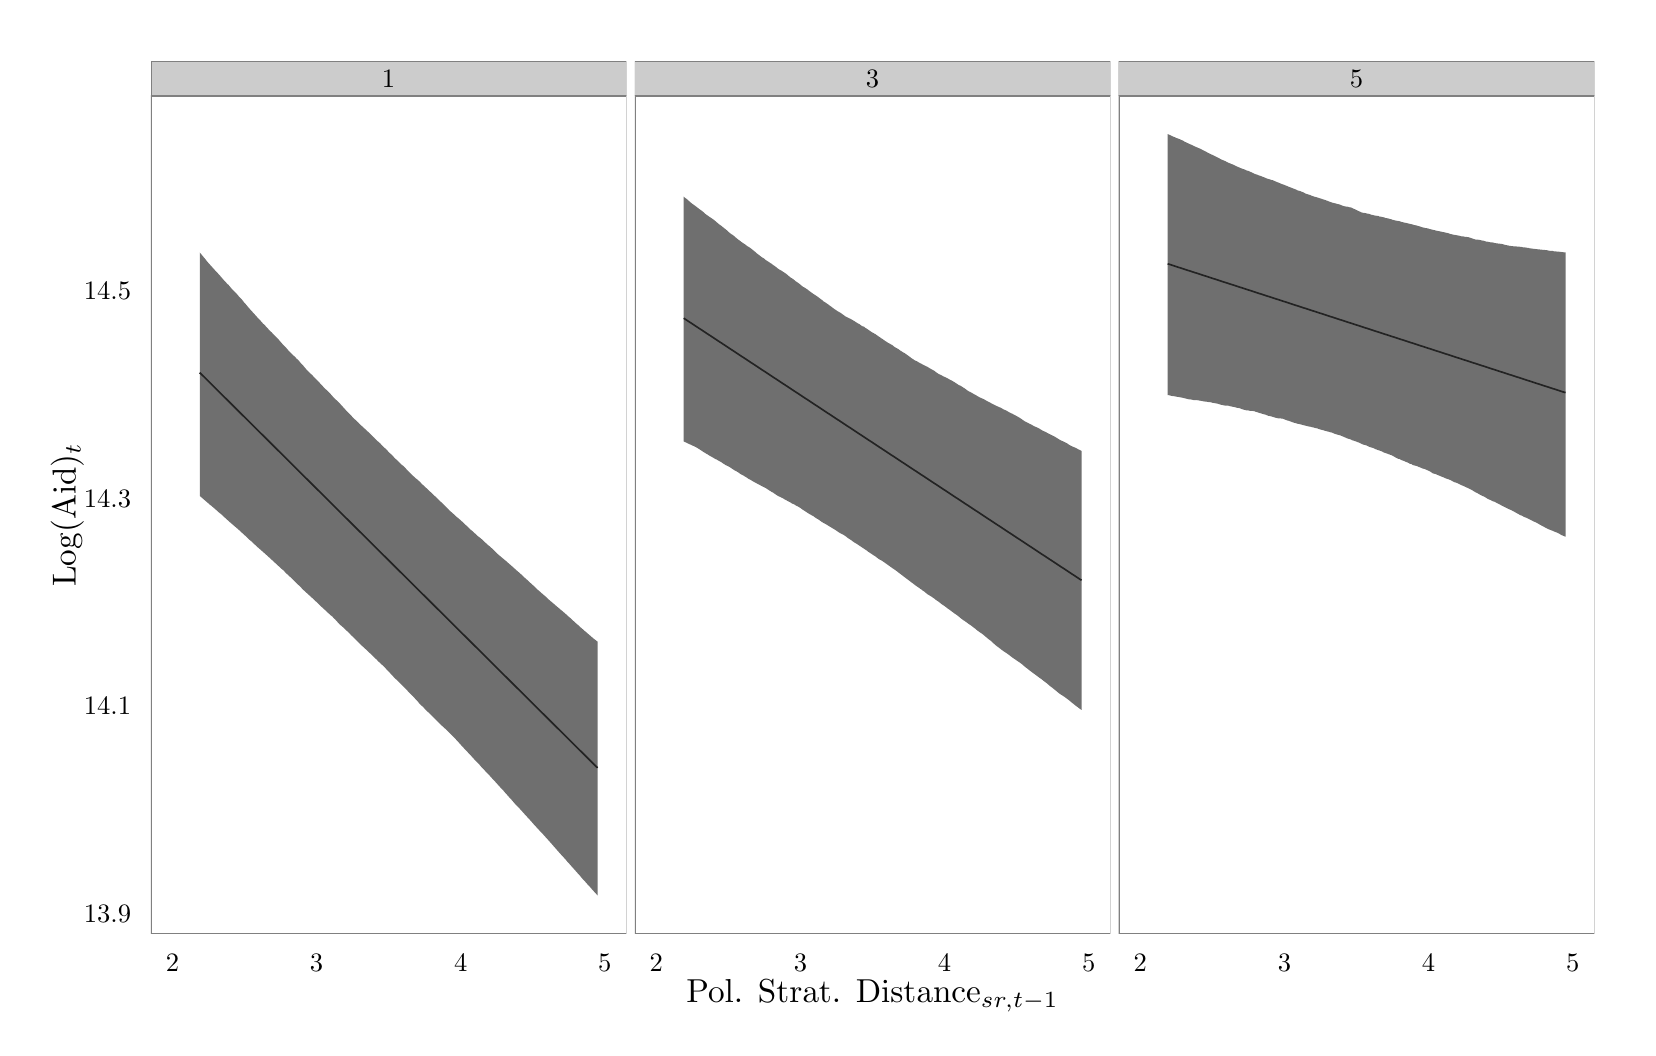
\begin{tikzpicture}[x=1pt,y=1pt]
\definecolor{fillColor}{RGB}{255,255,255}
\path[use as bounding box,fill=fillColor,fill opacity=0.00] (0,0) rectangle (578.16,361.35);
\begin{scope}
\path[clip] (  0.00,  0.00) rectangle (578.16,361.35);
\definecolor{drawColor}{RGB}{255,255,255}
\definecolor{fillColor}{RGB}{255,255,255}

\path[draw=drawColor,line width= 0.6pt,line join=round,line cap=round,fill=fillColor] (  0.00,  0.00) rectangle (578.16,361.35);
\end{scope}
\begin{scope}
\path[clip] ( 44.49,336.67) rectangle (216.35,349.31);
\definecolor{drawColor}{gray}{0.50}
\definecolor{fillColor}{gray}{0.80}

\path[draw=drawColor,line width= 0.2pt,line join=round,line cap=round,fill=fillColor] ( 44.49,336.67) rectangle (216.35,349.31);
\definecolor{drawColor}{RGB}{0,0,0}

\node[text=drawColor,anchor=base,inner sep=0pt, outer sep=0pt, scale=  0.96] at (130.42,339.68) {1};
\end{scope}
\begin{scope}
\path[clip] (219.37,336.67) rectangle (391.23,349.31);
\definecolor{drawColor}{gray}{0.50}
\definecolor{fillColor}{gray}{0.80}

\path[draw=drawColor,line width= 0.2pt,line join=round,line cap=round,fill=fillColor] (219.37,336.67) rectangle (391.23,349.31);
\definecolor{drawColor}{RGB}{0,0,0}

\node[text=drawColor,anchor=base,inner sep=0pt, outer sep=0pt, scale=  0.96] at (305.30,339.68) {3};
\end{scope}
\begin{scope}
\path[clip] (394.25,336.67) rectangle (566.12,349.31);
\definecolor{drawColor}{gray}{0.50}
\definecolor{fillColor}{gray}{0.80}

\path[draw=drawColor,line width= 0.2pt,line join=round,line cap=round,fill=fillColor] (394.25,336.67) rectangle (566.12,349.31);
\definecolor{drawColor}{RGB}{0,0,0}

\node[text=drawColor,anchor=base,inner sep=0pt, outer sep=0pt, scale=  0.96] at (480.18,339.68) {5};
\end{scope}
\begin{scope}
\path[clip] ( 44.49, 34.03) rectangle (216.35,336.67);
\definecolor{fillColor}{RGB}{255,255,255}

\path[fill=fillColor] ( 44.49, 34.03) rectangle (216.35,336.67);
\definecolor{drawColor}{RGB}{0,0,0}

\path[draw=drawColor,line width= 0.6pt,line join=round] ( 62.18,236.71) --
	( 62.70,236.19) --
	( 63.22,235.67) --
	( 63.74,235.16) --
	( 64.26,234.64) --
	( 64.78,234.12) --
	( 65.31,233.60) --
	( 65.83,233.09) --
	( 66.35,232.57) --
	( 66.87,232.05) --
	( 67.39,231.53) --
	( 67.91,231.02) --
	( 68.43,230.50) --
	( 68.95,229.98) --
	( 69.47,229.46) --
	( 69.99,228.95) --
	( 70.51,228.43) --
	( 71.03,227.91) --
	( 71.56,227.39) --
	( 72.08,226.88) --
	( 72.60,226.36) --
	( 73.12,225.84) --
	( 73.64,225.32) --
	( 74.16,224.81) --
	( 74.68,224.29) --
	( 75.20,223.77) --
	( 75.72,223.25) --
	( 76.24,222.74) --
	( 76.76,222.22) --
	( 77.28,221.70) --
	( 77.80,221.18) --
	( 78.33,220.67) --
	( 78.85,220.15) --
	( 79.37,219.63) --
	( 79.89,219.11) --
	( 80.41,218.60) --
	( 80.93,218.08) --
	( 81.45,217.56) --
	( 81.97,217.04) --
	( 82.49,216.53) --
	( 83.01,216.01) --
	( 83.53,215.49) --
	( 84.05,214.97) --
	( 84.58,214.46) --
	( 85.10,213.94) --
	( 85.62,213.42) --
	( 86.14,212.90) --
	( 86.66,212.39) --
	( 87.18,211.87) --
	( 87.70,211.35) --
	( 88.22,210.83) --
	( 88.74,210.32) --
	( 89.26,209.80) --
	( 89.78,209.28) --
	( 90.30,208.76) --
	( 90.83,208.25) --
	( 91.35,207.73) --
	( 91.87,207.21) --
	( 92.39,206.69) --
	( 92.91,206.18) --
	( 93.43,205.66) --
	( 93.95,205.14) --
	( 94.47,204.62) --
	( 94.99,204.11) --
	( 95.51,203.59) --
	( 96.03,203.07) --
	( 96.55,202.55) --
	( 97.07,202.04) --
	( 97.60,201.52) --
	( 98.12,201.00) --
	( 98.64,200.48) --
	( 99.16,199.97) --
	( 99.68,199.45) --
	(100.20,198.93) --
	(100.72,198.41) --
	(101.24,197.90) --
	(101.76,197.38) --
	(102.28,196.86) --
	(102.80,196.34) --
	(103.32,195.83) --
	(103.85,195.31) --
	(104.37,194.79) --
	(104.89,194.27) --
	(105.41,193.76) --
	(105.93,193.24) --
	(106.45,192.72) --
	(106.97,192.20) --
	(107.49,191.69) --
	(108.01,191.17) --
	(108.53,190.65) --
	(109.05,190.13) --
	(109.57,189.62) --
	(110.10,189.10) --
	(110.62,188.58) --
	(111.14,188.06) --
	(111.66,187.55) --
	(112.18,187.03) --
	(112.70,186.51) --
	(113.22,185.99) --
	(113.74,185.48) --
	(114.26,184.96) --
	(114.78,184.44) --
	(115.30,183.92) --
	(115.82,183.41) --
	(116.35,182.89) --
	(116.87,182.37) --
	(117.39,181.85) --
	(117.91,181.33) --
	(118.43,180.82) --
	(118.95,180.30) --
	(119.47,179.78) --
	(119.99,179.26) --
	(120.51,178.75) --
	(121.03,178.23) --
	(121.55,177.71) --
	(122.07,177.19) --
	(122.59,176.68) --
	(123.12,176.16) --
	(123.64,175.64) --
	(124.16,175.12) --
	(124.68,174.61) --
	(125.20,174.09) --
	(125.72,173.57) --
	(126.24,173.05) --
	(126.76,172.54) --
	(127.28,172.02) --
	(127.80,171.50) --
	(128.32,170.98) --
	(128.84,170.47) --
	(129.37,169.95) --
	(129.89,169.43) --
	(130.41,168.91) --
	(130.93,168.40) --
	(131.45,167.88) --
	(131.97,167.36) --
	(132.49,166.84) --
	(133.01,166.33) --
	(133.53,165.81) --
	(134.05,165.29) --
	(134.57,164.77) --
	(135.09,164.26) --
	(135.62,163.74) --
	(136.14,163.22) --
	(136.66,162.70) --
	(137.18,162.19) --
	(137.70,161.67) --
	(138.22,161.15) --
	(138.74,160.63) --
	(139.26,160.12) --
	(139.78,159.60) --
	(140.30,159.08) --
	(140.82,158.56) --
	(141.34,158.05) --
	(141.87,157.53) --
	(142.39,157.01) --
	(142.91,156.49) --
	(143.43,155.98) --
	(143.95,155.46) --
	(144.47,154.94) --
	(144.99,154.42) --
	(145.51,153.91) --
	(146.03,153.39) --
	(146.55,152.87) --
	(147.07,152.35) --
	(147.59,151.84) --
	(148.11,151.32) --
	(148.64,150.80) --
	(149.16,150.28) --
	(149.68,149.77) --
	(150.20,149.25) --
	(150.72,148.73) --
	(151.24,148.21) --
	(151.76,147.70) --
	(152.28,147.18) --
	(152.80,146.66) --
	(153.32,146.14) --
	(153.84,145.63) --
	(154.36,145.11) --
	(154.89,144.59) --
	(155.41,144.07) --
	(155.93,143.56) --
	(156.45,143.04) --
	(156.97,142.52) --
	(157.49,142.00) --
	(158.01,141.49) --
	(158.53,140.97) --
	(159.05,140.45) --
	(159.57,139.93) --
	(160.09,139.42) --
	(160.61,138.90) --
	(161.14,138.38) --
	(161.66,137.86) --
	(162.18,137.35) --
	(162.70,136.83) --
	(163.22,136.31) --
	(163.74,135.79) --
	(164.26,135.28) --
	(164.78,134.76) --
	(165.30,134.24) --
	(165.82,133.72) --
	(166.34,133.21) --
	(166.86,132.69) --
	(167.39,132.17) --
	(167.91,131.65) --
	(168.43,131.14) --
	(168.95,130.62) --
	(169.47,130.10) --
	(169.99,129.58) --
	(170.51,129.07) --
	(171.03,128.55) --
	(171.55,128.03) --
	(172.07,127.51) --
	(172.59,126.99) --
	(173.11,126.48) --
	(173.63,125.96) --
	(174.16,125.44) --
	(174.68,124.92) --
	(175.20,124.41) --
	(175.72,123.89) --
	(176.24,123.37) --
	(176.76,122.85) --
	(177.28,122.34) --
	(177.80,121.82) --
	(178.32,121.30) --
	(178.84,120.78) --
	(179.36,120.27) --
	(179.88,119.75) --
	(180.41,119.23) --
	(180.93,118.71) --
	(181.45,118.20) --
	(181.97,117.68) --
	(182.49,117.16) --
	(183.01,116.64) --
	(183.53,116.13) --
	(184.05,115.61) --
	(184.57,115.09) --
	(185.09,114.57) --
	(185.61,114.06) --
	(186.13,113.54) --
	(186.66,113.02) --
	(187.18,112.50) --
	(187.70,111.99) --
	(188.22,111.47) --
	(188.74,110.95) --
	(189.26,110.43) --
	(189.78,109.92) --
	(190.30,109.40) --
	(190.82,108.88) --
	(191.34,108.36) --
	(191.86,107.85) --
	(192.38,107.33) --
	(192.90,106.81) --
	(193.43,106.29) --
	(193.95,105.78) --
	(194.47,105.26) --
	(194.99,104.74) --
	(195.51,104.22) --
	(196.03,103.71) --
	(196.55,103.19) --
	(197.07,102.67) --
	(197.59,102.15) --
	(198.11,101.64) --
	(198.63,101.12) --
	(199.15,100.60) --
	(199.68,100.08) --
	(200.20, 99.57) --
	(200.72, 99.05) --
	(201.24, 98.53) --
	(201.76, 98.01) --
	(202.28, 97.50) --
	(202.80, 96.98) --
	(203.32, 96.46) --
	(203.84, 95.94) --
	(204.36, 95.43) --
	(204.88, 94.91) --
	(205.40, 94.39) --
	(205.93, 93.87);
\definecolor{fillColor}{RGB}{51,51,51}

\path[fill=fillColor,fill opacity=0.70] ( 62.18,280.11) --
	( 62.70,279.50) --
	( 63.22,278.87) --
	( 63.74,278.24) --
	( 64.26,277.61) --
	( 64.78,276.93) --
	( 65.31,276.33) --
	( 65.83,275.74) --
	( 66.35,275.17) --
	( 66.87,274.59) --
	( 67.39,274.01) --
	( 67.91,273.41) --
	( 68.43,272.90) --
	( 68.95,272.33) --
	( 69.47,271.76) --
	( 69.99,271.14) --
	( 70.51,270.54) --
	( 71.03,269.92) --
	( 71.56,269.38) --
	( 72.08,268.83) --
	( 72.60,268.35) --
	( 73.12,267.72) --
	( 73.64,267.10) --
	( 74.16,266.56) --
	( 74.68,266.02) --
	( 75.20,265.51) --
	( 75.72,264.94) --
	( 76.24,264.33) --
	( 76.76,263.75) --
	( 77.28,263.25) --
	( 77.80,262.60) --
	( 78.33,261.90) --
	( 78.85,261.36) --
	( 79.37,260.72) --
	( 79.89,260.11) --
	( 80.41,259.52) --
	( 80.93,258.96) --
	( 81.45,258.37) --
	( 81.97,257.80) --
	( 82.49,257.22) --
	( 83.01,256.63) --
	( 83.53,256.06) --
	( 84.05,255.56) --
	( 84.58,254.94) --
	( 85.10,254.36) --
	( 85.62,253.90) --
	( 86.14,253.33) --
	( 86.66,252.75) --
	( 87.18,252.20) --
	( 87.70,251.68) --
	( 88.22,251.18) --
	( 88.74,250.63) --
	( 89.26,250.12) --
	( 89.78,249.57) --
	( 90.30,249.07) --
	( 90.83,248.47) --
	( 91.35,247.86) --
	( 91.87,247.26) --
	( 92.39,246.69) --
	( 92.91,246.17) --
	( 93.43,245.62) --
	( 93.95,245.01) --
	( 94.47,244.41) --
	( 94.99,243.90) --
	( 95.51,243.42) --
	( 96.03,242.89) --
	( 96.55,242.44) --
	( 97.07,241.86) --
	( 97.60,241.36) --
	( 98.12,240.83) --
	( 98.64,240.18) --
	( 99.16,239.69) --
	( 99.68,239.08) --
	(100.20,238.45) --
	(100.72,237.83) --
	(101.24,237.30) --
	(101.76,236.78) --
	(102.28,236.28) --
	(102.80,235.81) --
	(103.32,235.23) --
	(103.85,234.70) --
	(104.37,234.19) --
	(104.89,233.67) --
	(105.41,233.12) --
	(105.93,232.49) --
	(106.45,231.97) --
	(106.97,231.41) --
	(107.49,230.85) --
	(108.01,230.41) --
	(108.53,229.94) --
	(109.05,229.40) --
	(109.57,228.83) --
	(110.10,228.22) --
	(110.62,227.64) --
	(111.14,227.13) --
	(111.66,226.66) --
	(112.18,226.15) --
	(112.70,225.65) --
	(113.22,225.07) --
	(113.74,224.49) --
	(114.26,223.92) --
	(114.78,223.35) --
	(115.30,222.79) --
	(115.82,222.26) --
	(116.35,221.72) --
	(116.87,221.19) --
	(117.39,220.63) --
	(117.91,220.05) --
	(118.43,219.62) --
	(118.95,219.13) --
	(119.47,218.66) --
	(119.99,218.09) --
	(120.51,217.60) --
	(121.03,217.14) --
	(121.55,216.63) --
	(122.07,216.19) --
	(122.59,215.70) --
	(123.12,215.20) --
	(123.64,214.70) --
	(124.16,214.19) --
	(124.68,213.70) --
	(125.20,213.20) --
	(125.72,212.67) --
	(126.24,212.12) --
	(126.76,211.66) --
	(127.28,211.22) --
	(127.80,210.68) --
	(128.32,210.11) --
	(128.84,209.62) --
	(129.37,209.16) --
	(129.89,208.64) --
	(130.41,208.05) --
	(130.93,207.55) --
	(131.45,207.06) --
	(131.97,206.53) --
	(132.49,205.99) --
	(133.01,205.47) --
	(133.53,204.98) --
	(134.05,204.45) --
	(134.57,204.00) --
	(135.09,203.46) --
	(135.62,203.07) --
	(136.14,202.56) --
	(136.66,202.02) --
	(137.18,201.45) --
	(137.70,200.88) --
	(138.22,200.41) --
	(138.74,199.89) --
	(139.26,199.38) --
	(139.78,198.93) --
	(140.30,198.45) --
	(140.82,198.06) --
	(141.34,197.59) --
	(141.87,197.09) --
	(142.39,196.51) --
	(142.91,196.03) --
	(143.43,195.55) --
	(143.95,195.07) --
	(144.47,194.60) --
	(144.99,194.11) --
	(145.51,193.61) --
	(146.03,193.15) --
	(146.55,192.66) --
	(147.07,192.14) --
	(147.59,191.64) --
	(148.11,191.13) --
	(148.64,190.63) --
	(149.16,190.10) --
	(149.68,189.67) --
	(150.20,189.14) --
	(150.72,188.60) --
	(151.24,188.14) --
	(151.76,187.63) --
	(152.28,187.01) --
	(152.80,186.56) --
	(153.32,186.09) --
	(153.84,185.64) --
	(154.36,185.18) --
	(154.89,184.65) --
	(155.41,184.25) --
	(155.93,183.80) --
	(156.45,183.37) --
	(156.97,182.88) --
	(157.49,182.39) --
	(158.01,181.90) --
	(158.53,181.41) --
	(159.05,180.93) --
	(159.57,180.45) --
	(160.09,179.93) --
	(160.61,179.51) --
	(161.14,179.00) --
	(161.66,178.55) --
	(162.18,178.09) --
	(162.70,177.59) --
	(163.22,177.18) --
	(163.74,176.81) --
	(164.26,176.32) --
	(164.78,175.83) --
	(165.30,175.35) --
	(165.82,174.85) --
	(166.34,174.37) --
	(166.86,173.99) --
	(167.39,173.53) --
	(167.91,173.03) --
	(168.43,172.53) --
	(168.95,172.03) --
	(169.47,171.53) --
	(169.99,171.02) --
	(170.51,170.57) --
	(171.03,170.14) --
	(171.55,169.70) --
	(172.07,169.26) --
	(172.59,168.84) --
	(173.11,168.39) --
	(173.63,167.92) --
	(174.16,167.48) --
	(174.68,166.99) --
	(175.20,166.56) --
	(175.72,166.08) --
	(176.24,165.64) --
	(176.76,165.16) --
	(177.28,164.72) --
	(177.80,164.24) --
	(178.32,163.80) --
	(178.84,163.34) --
	(179.36,162.80) --
	(179.88,162.34) --
	(180.41,161.88) --
	(180.93,161.41) --
	(181.45,160.90) --
	(181.97,160.43) --
	(182.49,159.96) --
	(183.01,159.48) --
	(183.53,159.01) --
	(184.05,158.42) --
	(184.57,158.01) --
	(185.09,157.57) --
	(185.61,157.09) --
	(186.13,156.65) --
	(186.66,156.19) --
	(187.18,155.75) --
	(187.70,155.26) --
	(188.22,154.75) --
	(188.74,154.31) --
	(189.26,153.87) --
	(189.78,153.43) --
	(190.30,152.99) --
	(190.82,152.54) --
	(191.34,152.10) --
	(191.86,151.66) --
	(192.38,151.22) --
	(192.90,150.78) --
	(193.43,150.35) --
	(193.95,149.89) --
	(194.47,149.44) --
	(194.99,148.97) --
	(195.51,148.49) --
	(196.03,148.06) --
	(196.55,147.56) --
	(197.07,147.09) --
	(197.59,146.62) --
	(198.11,146.13) --
	(198.63,145.71) --
	(199.15,145.24) --
	(199.68,144.74) --
	(200.20,144.31) --
	(200.72,143.84) --
	(201.24,143.38) --
	(201.76,142.95) --
	(202.28,142.50) --
	(202.80,142.04) --
	(203.32,141.61) --
	(203.84,141.15) --
	(204.36,140.68) --
	(204.88,140.31) --
	(205.40,139.91) --
	(205.93,139.46) --
	(205.93, 47.79) --
	(205.40, 48.37) --
	(204.88, 48.94) --
	(204.36, 49.51) --
	(203.84, 50.09) --
	(203.32, 50.71) --
	(202.80, 51.27) --
	(202.28, 51.81) --
	(201.76, 52.42) --
	(201.24, 52.99) --
	(200.72, 53.53) --
	(200.20, 54.15) --
	(199.68, 54.78) --
	(199.15, 55.37) --
	(198.63, 55.94) --
	(198.11, 56.53) --
	(197.59, 57.11) --
	(197.07, 57.71) --
	(196.55, 58.28) --
	(196.03, 58.86) --
	(195.51, 59.50) --
	(194.99, 60.02) --
	(194.47, 60.66) --
	(193.95, 61.22) --
	(193.43, 61.84) --
	(192.90, 62.37) --
	(192.38, 62.93) --
	(191.86, 63.53) --
	(191.34, 64.12) --
	(190.82, 64.72) --
	(190.30, 65.31) --
	(189.78, 65.90) --
	(189.26, 66.50) --
	(188.74, 67.08) --
	(188.22, 67.67) --
	(187.70, 68.25) --
	(187.18, 68.80) --
	(186.66, 69.43) --
	(186.13, 69.98) --
	(185.61, 70.57) --
	(185.09, 71.08) --
	(184.57, 71.67) --
	(184.05, 72.21) --
	(183.53, 72.79) --
	(183.01, 73.34) --
	(182.49, 73.92) --
	(181.97, 74.56) --
	(181.45, 75.11) --
	(180.93, 75.67) --
	(180.41, 76.24) --
	(179.88, 76.83) --
	(179.36, 77.38) --
	(178.84, 77.98) --
	(178.32, 78.56) --
	(177.80, 79.12) --
	(177.28, 79.67) --
	(176.76, 80.16) --
	(176.24, 80.71) --
	(175.72, 81.33) --
	(175.20, 81.93) --
	(174.68, 82.55) --
	(174.16, 83.07) --
	(173.63, 83.70) --
	(173.11, 84.27) --
	(172.59, 84.84) --
	(172.07, 85.47) --
	(171.55, 86.04) --
	(171.03, 86.59) --
	(170.51, 87.14) --
	(169.99, 87.73) --
	(169.47, 88.28) --
	(168.95, 88.87) --
	(168.43, 89.46) --
	(167.91, 89.99) --
	(167.39, 90.57) --
	(166.86, 91.15) --
	(166.34, 91.71) --
	(165.82, 92.20) --
	(165.30, 92.78) --
	(164.78, 93.37) --
	(164.26, 93.88) --
	(163.74, 94.44) --
	(163.22, 95.07) --
	(162.70, 95.63) --
	(162.18, 96.12) --
	(161.66, 96.67) --
	(161.14, 97.23) --
	(160.61, 97.83) --
	(160.09, 98.39) --
	(159.57, 98.96) --
	(159.05, 99.49) --
	(158.53,100.04) --
	(158.01,100.57) --
	(157.49,101.16) --
	(156.97,101.70) --
	(156.45,102.29) --
	(155.93,102.87) --
	(155.41,103.44) --
	(154.89,104.01) --
	(154.36,104.58) --
	(153.84,105.13) --
	(153.32,105.65) --
	(152.80,106.15) --
	(152.28,106.65) --
	(151.76,107.16) --
	(151.24,107.67) --
	(150.72,108.18) --
	(150.20,108.66) --
	(149.68,109.11) --
	(149.16,109.60) --
	(148.64,110.13) --
	(148.11,110.66) --
	(147.59,111.18) --
	(147.07,111.68) --
	(146.55,112.22) --
	(146.03,112.71) --
	(145.51,113.25) --
	(144.99,113.76) --
	(144.47,114.23) --
	(143.95,114.77) --
	(143.43,115.28) --
	(142.91,115.85) --
	(142.39,116.33) --
	(141.87,116.82) --
	(141.34,117.38) --
	(140.82,118.03) --
	(140.30,118.54) --
	(139.78,119.14) --
	(139.26,119.74) --
	(138.74,120.20) --
	(138.22,120.77) --
	(137.70,121.27) --
	(137.18,121.82) --
	(136.66,122.35) --
	(136.14,122.86) --
	(135.62,123.38) --
	(135.09,123.97) --
	(134.57,124.51) --
	(134.05,124.99) --
	(133.53,125.51) --
	(133.01,125.97) --
	(132.49,126.48) --
	(131.97,127.04) --
	(131.45,127.60) --
	(130.93,128.17) --
	(130.41,128.73) --
	(129.89,129.24) --
	(129.37,129.81) --
	(128.84,130.35) --
	(128.32,130.87) --
	(127.80,131.36) --
	(127.28,131.86) --
	(126.76,132.31) --
	(126.24,132.85) --
	(125.72,133.36) --
	(125.20,133.86) --
	(124.68,134.39) --
	(124.16,134.87) --
	(123.64,135.35) --
	(123.12,135.85) --
	(122.59,136.34) --
	(122.07,136.83) --
	(121.55,137.31) --
	(121.03,137.78) --
	(120.51,138.27) --
	(119.99,138.82) --
	(119.47,139.30) --
	(118.95,139.79) --
	(118.43,140.36) --
	(117.91,140.90) --
	(117.39,141.39) --
	(116.87,141.83) --
	(116.35,142.42) --
	(115.82,142.95) --
	(115.30,143.42) --
	(114.78,143.92) --
	(114.26,144.42) --
	(113.74,144.88) --
	(113.22,145.32) --
	(112.70,145.74) --
	(112.18,146.33) --
	(111.66,146.92) --
	(111.14,147.50) --
	(110.62,147.98) --
	(110.10,148.55) --
	(109.57,148.95) --
	(109.05,149.45) --
	(108.53,149.89) --
	(108.01,150.41) --
	(107.49,150.91) --
	(106.97,151.30) --
	(106.45,151.85) --
	(105.93,152.27) --
	(105.41,152.80) --
	(104.89,153.29) --
	(104.37,153.82) --
	(103.85,154.30) --
	(103.32,154.81) --
	(102.80,155.29) --
	(102.28,155.77) --
	(101.76,156.24) --
	(101.24,156.71) --
	(100.72,157.18) --
	(100.20,157.64) --
	( 99.68,158.13) --
	( 99.16,158.64) --
	( 98.64,159.22) --
	( 98.12,159.72) --
	( 97.60,160.18) --
	( 97.07,160.69) --
	( 96.55,161.20) --
	( 96.03,161.70) --
	( 95.51,162.23) --
	( 94.99,162.76) --
	( 94.47,163.22) --
	( 93.95,163.71) --
	( 93.43,164.16) --
	( 92.91,164.72) --
	( 92.39,165.29) --
	( 91.87,165.70) --
	( 91.35,166.14) --
	( 90.83,166.64) --
	( 90.30,167.12) --
	( 89.78,167.61) --
	( 89.26,168.08) --
	( 88.74,168.56) --
	( 88.22,169.05) --
	( 87.70,169.55) --
	( 87.18,169.99) --
	( 86.66,170.50) --
	( 86.14,170.94) --
	( 85.62,171.42) --
	( 85.10,171.85) --
	( 84.58,172.33) --
	( 84.05,172.80) --
	( 83.53,173.25) --
	( 83.01,173.69) --
	( 82.49,174.22) --
	( 81.97,174.66) --
	( 81.45,175.15) --
	( 80.93,175.64) --
	( 80.41,176.11) --
	( 79.89,176.50) --
	( 79.37,177.02) --
	( 78.85,177.54) --
	( 78.33,178.03) --
	( 77.80,178.50) --
	( 77.28,178.97) --
	( 76.76,179.46) --
	( 76.24,179.94) --
	( 75.72,180.39) --
	( 75.20,180.83) --
	( 74.68,181.27) --
	( 74.16,181.74) --
	( 73.64,182.19) --
	( 73.12,182.61) --
	( 72.60,183.09) --
	( 72.08,183.55) --
	( 71.56,184.02) --
	( 71.03,184.52) --
	( 70.51,185.00) --
	( 69.99,185.48) --
	( 69.47,185.90) --
	( 68.95,186.30) --
	( 68.43,186.80) --
	( 67.91,187.26) --
	( 67.39,187.71) --
	( 66.87,188.15) --
	( 66.35,188.59) --
	( 65.83,188.99) --
	( 65.31,189.45) --
	( 64.78,189.90) --
	( 64.26,190.35) --
	( 63.74,190.80) --
	( 63.22,191.26) --
	( 62.70,191.71) --
	( 62.18,192.17) --
	cycle;
\definecolor{drawColor}{gray}{0.50}

\path[draw=drawColor,line width= 0.6pt,line join=round,line cap=round] ( 44.49, 34.03) rectangle (216.35,336.67);
\end{scope}
\begin{scope}
\path[clip] (219.37, 34.03) rectangle (391.23,336.67);
\definecolor{fillColor}{RGB}{255,255,255}

\path[fill=fillColor] (219.37, 34.03) rectangle (391.23,336.67);
\definecolor{drawColor}{RGB}{0,0,0}

\path[draw=drawColor,line width= 0.6pt,line join=round] (237.06,256.37) --
	(237.58,256.02) --
	(238.10,255.68) --
	(238.62,255.34) --
	(239.14,254.99) --
	(239.66,254.65) --
	(240.19,254.31) --
	(240.71,253.97) --
	(241.23,253.62) --
	(241.75,253.28) --
	(242.27,252.94) --
	(242.79,252.59) --
	(243.31,252.25) --
	(243.83,251.91) --
	(244.35,251.56) --
	(244.87,251.22) --
	(245.39,250.88) --
	(245.91,250.53) --
	(246.44,250.19) --
	(246.96,249.85) --
	(247.48,249.50) --
	(248.00,249.16) --
	(248.52,248.82) --
	(249.04,248.48) --
	(249.56,248.13) --
	(250.08,247.79) --
	(250.60,247.45) --
	(251.12,247.10) --
	(251.64,246.76) --
	(252.16,246.42) --
	(252.69,246.07) --
	(253.21,245.73) --
	(253.73,245.39) --
	(254.25,245.04) --
	(254.77,244.70) --
	(255.29,244.36) --
	(255.81,244.01) --
	(256.33,243.67) --
	(256.85,243.33) --
	(257.37,242.98) --
	(257.89,242.64) --
	(258.41,242.30) --
	(258.93,241.96) --
	(259.46,241.61) --
	(259.98,241.27) --
	(260.50,240.93) --
	(261.02,240.58) --
	(261.54,240.24) --
	(262.06,239.90) --
	(262.58,239.55) --
	(263.10,239.21) --
	(263.62,238.87) --
	(264.14,238.52) --
	(264.66,238.18) --
	(265.18,237.84) --
	(265.71,237.49) --
	(266.23,237.15) --
	(266.75,236.81) --
	(267.27,236.47) --
	(267.79,236.12) --
	(268.31,235.78) --
	(268.83,235.44) --
	(269.35,235.09) --
	(269.87,234.75) --
	(270.39,234.41) --
	(270.91,234.06) --
	(271.43,233.72) --
	(271.96,233.38) --
	(272.48,233.03) --
	(273.00,232.69) --
	(273.52,232.35) --
	(274.04,232.00) --
	(274.56,231.66) --
	(275.08,231.32) --
	(275.60,230.97) --
	(276.12,230.63) --
	(276.64,230.29) --
	(277.16,229.95) --
	(277.68,229.60) --
	(278.21,229.26) --
	(278.73,228.92) --
	(279.25,228.57) --
	(279.77,228.23) --
	(280.29,227.89) --
	(280.81,227.54) --
	(281.33,227.20) --
	(281.85,226.86) --
	(282.37,226.51) --
	(282.89,226.17) --
	(283.41,225.83) --
	(283.93,225.48) --
	(284.45,225.14) --
	(284.98,224.80) --
	(285.50,224.46) --
	(286.02,224.11) --
	(286.54,223.77) --
	(287.06,223.43) --
	(287.58,223.08) --
	(288.10,222.74) --
	(288.62,222.40) --
	(289.14,222.05) --
	(289.66,221.71) --
	(290.18,221.37) --
	(290.70,221.02) --
	(291.23,220.68) --
	(291.75,220.34) --
	(292.27,219.99) --
	(292.79,219.65) --
	(293.31,219.31) --
	(293.83,218.96) --
	(294.35,218.62) --
	(294.87,218.28) --
	(295.39,217.94) --
	(295.91,217.59) --
	(296.43,217.25) --
	(296.95,216.91) --
	(297.48,216.56) --
	(298.00,216.22) --
	(298.52,215.88) --
	(299.04,215.53) --
	(299.56,215.19) --
	(300.08,214.85) --
	(300.60,214.50) --
	(301.12,214.16) --
	(301.64,213.82) --
	(302.16,213.47) --
	(302.68,213.13) --
	(303.20,212.79) --
	(303.72,212.45) --
	(304.25,212.10) --
	(304.77,211.76) --
	(305.29,211.42) --
	(305.81,211.07) --
	(306.33,210.73) --
	(306.85,210.39) --
	(307.37,210.04) --
	(307.89,209.70) --
	(308.41,209.36) --
	(308.93,209.01) --
	(309.45,208.67) --
	(309.97,208.33) --
	(310.50,207.98) --
	(311.02,207.64) --
	(311.54,207.30) --
	(312.06,206.95) --
	(312.58,206.61) --
	(313.10,206.27) --
	(313.62,205.93) --
	(314.14,205.58) --
	(314.66,205.24) --
	(315.18,204.90) --
	(315.70,204.55) --
	(316.22,204.21) --
	(316.75,203.87) --
	(317.27,203.52) --
	(317.79,203.18) --
	(318.31,202.84) --
	(318.83,202.49) --
	(319.35,202.15) --
	(319.87,201.81) --
	(320.39,201.46) --
	(320.91,201.12) --
	(321.43,200.78) --
	(321.95,200.44) --
	(322.47,200.09) --
	(323.00,199.75) --
	(323.52,199.41) --
	(324.04,199.06) --
	(324.56,198.72) --
	(325.08,198.38) --
	(325.60,198.03) --
	(326.12,197.69) --
	(326.64,197.35) --
	(327.16,197.00) --
	(327.68,196.66) --
	(328.20,196.32) --
	(328.72,195.97) --
	(329.24,195.63) --
	(329.77,195.29) --
	(330.29,194.94) --
	(330.81,194.60) --
	(331.33,194.26) --
	(331.85,193.92) --
	(332.37,193.57) --
	(332.89,193.23) --
	(333.41,192.89) --
	(333.93,192.54) --
	(334.45,192.20) --
	(334.97,191.86) --
	(335.49,191.51) --
	(336.02,191.17) --
	(336.54,190.83) --
	(337.06,190.48) --
	(337.58,190.14) --
	(338.10,189.80) --
	(338.62,189.45) --
	(339.14,189.11) --
	(339.66,188.77) --
	(340.18,188.43) --
	(340.70,188.08) --
	(341.22,187.74) --
	(341.74,187.40) --
	(342.27,187.05) --
	(342.79,186.71) --
	(343.31,186.37) --
	(343.83,186.02) --
	(344.35,185.68) --
	(344.87,185.34) --
	(345.39,184.99) --
	(345.91,184.65) --
	(346.43,184.31) --
	(346.95,183.96) --
	(347.47,183.62) --
	(347.99,183.28) --
	(348.52,182.93) --
	(349.04,182.59) --
	(349.56,182.25) --
	(350.08,181.91) --
	(350.60,181.56) --
	(351.12,181.22) --
	(351.64,180.88) --
	(352.16,180.53) --
	(352.68,180.19) --
	(353.20,179.85) --
	(353.72,179.50) --
	(354.24,179.16) --
	(354.76,178.82) --
	(355.29,178.47) --
	(355.81,178.13) --
	(356.33,177.79) --
	(356.85,177.44) --
	(357.37,177.10) --
	(357.89,176.76) --
	(358.41,176.42) --
	(358.93,176.07) --
	(359.45,175.73) --
	(359.97,175.39) --
	(360.49,175.04) --
	(361.01,174.70) --
	(361.54,174.36) --
	(362.06,174.01) --
	(362.58,173.67) --
	(363.10,173.33) --
	(363.62,172.98) --
	(364.14,172.64) --
	(364.66,172.30) --
	(365.18,171.95) --
	(365.70,171.61) --
	(366.22,171.27) --
	(366.74,170.92) --
	(367.26,170.58) --
	(367.79,170.24) --
	(368.31,169.90) --
	(368.83,169.55) --
	(369.35,169.21) --
	(369.87,168.87) --
	(370.39,168.52) --
	(370.91,168.18) --
	(371.43,167.84) --
	(371.95,167.49) --
	(372.47,167.15) --
	(372.99,166.81) --
	(373.51,166.46) --
	(374.04,166.12) --
	(374.56,165.78) --
	(375.08,165.43) --
	(375.60,165.09) --
	(376.12,164.75) --
	(376.64,164.41) --
	(377.16,164.06) --
	(377.68,163.72) --
	(378.20,163.38) --
	(378.72,163.03) --
	(379.24,162.69) --
	(379.76,162.35) --
	(380.28,162.00) --
	(380.81,161.66);
\definecolor{fillColor}{RGB}{51,51,51}

\path[fill=fillColor,fill opacity=0.70] (237.06,300.27) --
	(237.58,299.84) --
	(238.10,299.46) --
	(238.62,299.01) --
	(239.14,298.55) --
	(239.66,298.09) --
	(240.19,297.68) --
	(240.71,297.31) --
	(241.23,296.95) --
	(241.75,296.52) --
	(242.27,296.13) --
	(242.79,295.72) --
	(243.31,295.37) --
	(243.83,294.98) --
	(244.35,294.55) --
	(244.87,294.04) --
	(245.39,293.67) --
	(245.91,293.31) --
	(246.44,292.94) --
	(246.96,292.59) --
	(247.48,292.26) --
	(248.00,291.86) --
	(248.52,291.42) --
	(249.04,290.98) --
	(249.56,290.54) --
	(250.08,290.13) --
	(250.60,289.77) --
	(251.12,289.35) --
	(251.64,288.91) --
	(252.16,288.53) --
	(252.69,288.08) --
	(253.21,287.59) --
	(253.73,287.13) --
	(254.25,286.74) --
	(254.77,286.45) --
	(255.29,286.01) --
	(255.81,285.56) --
	(256.33,285.11) --
	(256.85,284.71) --
	(257.37,284.35) --
	(257.89,283.90) --
	(258.41,283.56) --
	(258.93,283.24) --
	(259.46,282.87) --
	(259.98,282.42) --
	(260.50,282.13) --
	(261.02,281.80) --
	(261.54,281.41) --
	(262.06,280.99) --
	(262.58,280.58) --
	(263.10,280.13) --
	(263.62,279.67) --
	(264.14,279.29) --
	(264.66,278.87) --
	(265.18,278.47) --
	(265.71,278.14) --
	(266.23,277.81) --
	(266.75,277.35) --
	(267.27,277.03) --
	(267.79,276.69) --
	(268.31,276.34) --
	(268.83,276.02) --
	(269.35,275.58) --
	(269.87,275.26) --
	(270.39,274.87) --
	(270.91,274.43) --
	(271.43,274.06) --
	(271.96,273.74) --
	(272.48,273.47) --
	(273.00,273.10) --
	(273.52,272.77) --
	(274.04,272.42) --
	(274.56,271.99) --
	(275.08,271.55) --
	(275.60,271.10) --
	(276.12,270.82) --
	(276.64,270.45) --
	(277.16,270.02) --
	(277.68,269.60) --
	(278.21,269.25) --
	(278.73,268.89) --
	(279.25,268.47) --
	(279.77,268.00) --
	(280.29,267.63) --
	(280.81,267.36) --
	(281.33,267.01) --
	(281.85,266.68) --
	(282.37,266.26) --
	(282.89,265.86) --
	(283.41,265.48) --
	(283.93,265.12) --
	(284.45,264.81) --
	(284.98,264.43) --
	(285.50,264.09) --
	(286.02,263.68) --
	(286.54,263.28) --
	(287.06,262.92) --
	(287.58,262.43) --
	(288.10,262.14) --
	(288.62,261.77) --
	(289.14,261.43) --
	(289.66,261.03) --
	(290.18,260.67) --
	(290.70,260.27) --
	(291.23,259.86) --
	(291.75,259.49) --
	(292.27,259.18) --
	(292.79,258.81) --
	(293.31,258.53) --
	(293.83,258.25) --
	(294.35,257.84) --
	(294.87,257.48) --
	(295.39,257.07) --
	(295.91,256.81) --
	(296.43,256.53) --
	(296.95,256.27) --
	(297.48,256.05) --
	(298.00,255.72) --
	(298.52,255.43) --
	(299.04,255.10) --
	(299.56,254.76) --
	(300.08,254.45) --
	(300.60,254.17) --
	(301.12,253.78) --
	(301.64,253.46) --
	(302.16,253.31) --
	(302.68,252.89) --
	(303.20,252.57) --
	(303.72,252.23) --
	(304.25,251.85) --
	(304.77,251.47) --
	(305.29,251.16) --
	(305.81,250.89) --
	(306.33,250.59) --
	(306.85,250.22) --
	(307.37,249.86) --
	(307.89,249.50) --
	(308.41,249.13) --
	(308.93,248.81) --
	(309.45,248.43) --
	(309.97,248.06) --
	(310.50,247.73) --
	(311.02,247.40) --
	(311.54,247.12) --
	(312.06,246.85) --
	(312.58,246.53) --
	(313.10,246.08) --
	(313.62,245.74) --
	(314.14,245.47) --
	(314.66,245.17) --
	(315.18,244.76) --
	(315.70,244.44) --
	(316.22,244.08) --
	(316.75,243.83) --
	(317.27,243.45) --
	(317.79,243.09) --
	(318.31,242.72) --
	(318.83,242.34) --
	(319.35,241.91) --
	(319.87,241.62) --
	(320.39,241.22) --
	(320.91,240.96) --
	(321.43,240.75) --
	(321.95,240.40) --
	(322.47,240.11) --
	(323.00,239.86) --
	(323.52,239.57) --
	(324.04,239.30) --
	(324.56,239.05) --
	(325.08,238.82) --
	(325.60,238.48) --
	(326.12,238.18) --
	(326.64,237.87) --
	(327.16,237.60) --
	(327.68,237.29) --
	(328.20,236.87) --
	(328.72,236.52) --
	(329.24,236.18) --
	(329.77,235.94) --
	(330.29,235.69) --
	(330.81,235.36) --
	(331.33,235.15) --
	(331.85,234.90) --
	(332.37,234.64) --
	(332.89,234.35) --
	(333.41,234.05) --
	(333.93,233.81) --
	(334.45,233.51) --
	(334.97,233.18) --
	(335.49,232.86) --
	(336.02,232.50) --
	(336.54,232.14) --
	(337.06,231.97) --
	(337.58,231.62) --
	(338.10,231.28) --
	(338.62,230.99) --
	(339.14,230.57) --
	(339.66,230.18) --
	(340.18,229.89) --
	(340.70,229.65) --
	(341.22,229.35) --
	(341.74,229.03) --
	(342.27,228.75) --
	(342.79,228.46) --
	(343.31,228.13) --
	(343.83,227.84) --
	(344.35,227.60) --
	(344.87,227.36) --
	(345.39,227.15) --
	(345.91,226.86) --
	(346.43,226.54) --
	(346.95,226.27) --
	(347.47,226.00) --
	(347.99,225.73) --
	(348.52,225.46) --
	(349.04,225.20) --
	(349.56,224.92) --
	(350.08,224.65) --
	(350.60,224.44) --
	(351.12,224.19) --
	(351.64,224.00) --
	(352.16,223.68) --
	(352.68,223.38) --
	(353.20,223.16) --
	(353.72,222.94) --
	(354.24,222.62) --
	(354.76,222.31) --
	(355.29,222.06) --
	(355.81,221.83) --
	(356.33,221.55) --
	(356.85,221.27) --
	(357.37,220.98) --
	(357.89,220.70) --
	(358.41,220.40) --
	(358.93,220.06) --
	(359.45,219.67) --
	(359.97,219.31) --
	(360.49,218.99) --
	(361.01,218.74) --
	(361.54,218.48) --
	(362.06,218.18) --
	(362.58,217.97) --
	(363.10,217.67) --
	(363.62,217.36) --
	(364.14,217.14) --
	(364.66,216.91) --
	(365.18,216.65) --
	(365.70,216.38) --
	(366.22,216.03) --
	(366.74,215.76) --
	(367.26,215.50) --
	(367.79,215.26) --
	(368.31,214.98) --
	(368.83,214.70) --
	(369.35,214.43) --
	(369.87,214.17) --
	(370.39,213.90) --
	(370.91,213.68) --
	(371.43,213.37) --
	(371.95,213.04) --
	(372.47,212.71) --
	(372.99,212.39) --
	(373.51,212.12) --
	(374.04,211.90) --
	(374.56,211.65) --
	(375.08,211.40) --
	(375.60,211.13) --
	(376.12,210.76) --
	(376.64,210.42) --
	(377.16,210.19) --
	(377.68,209.93) --
	(378.20,209.71) --
	(378.72,209.49) --
	(379.24,209.21) --
	(379.76,208.92) --
	(380.28,208.70) --
	(380.81,208.39) --
	(380.81,114.79) --
	(380.28,115.18) --
	(379.76,115.55) --
	(379.24,115.96) --
	(378.72,116.33) --
	(378.20,116.74) --
	(377.68,117.16) --
	(377.16,117.58) --
	(376.64,118.02) --
	(376.12,118.45) --
	(375.60,118.84) --
	(375.08,119.22) --
	(374.56,119.60) --
	(374.04,119.95) --
	(373.51,120.27) --
	(372.99,120.61) --
	(372.47,121.00) --
	(371.95,121.42) --
	(371.43,121.88) --
	(370.91,122.29) --
	(370.39,122.72) --
	(369.87,123.12) --
	(369.35,123.49) --
	(368.83,123.96) --
	(368.31,124.41) --
	(367.79,124.80) --
	(367.26,125.20) --
	(366.74,125.61) --
	(366.22,126.02) --
	(365.70,126.38) --
	(365.18,126.75) --
	(364.66,127.15) --
	(364.14,127.53) --
	(363.62,127.92) --
	(363.10,128.30) --
	(362.58,128.69) --
	(362.06,129.07) --
	(361.54,129.50) --
	(361.01,129.91) --
	(360.49,130.30) --
	(359.97,130.75) --
	(359.45,131.21) --
	(358.93,131.62) --
	(358.41,131.99) --
	(357.89,132.33) --
	(357.37,132.67) --
	(356.85,133.06) --
	(356.33,133.40) --
	(355.81,133.77) --
	(355.29,134.16) --
	(354.76,134.58) --
	(354.24,134.94) --
	(353.72,135.32) --
	(353.20,135.66) --
	(352.68,136.00) --
	(352.16,136.38) --
	(351.64,136.75) --
	(351.12,137.20) --
	(350.60,137.57) --
	(350.08,137.95) --
	(349.56,138.40) --
	(349.04,138.86) --
	(348.52,139.36) --
	(347.99,139.83) --
	(347.47,140.19) --
	(346.95,140.60) --
	(346.43,141.06) --
	(345.91,141.48) --
	(345.39,141.93) --
	(344.87,142.33) --
	(344.35,142.68) --
	(343.83,143.04) --
	(343.31,143.42) --
	(342.79,143.83) --
	(342.27,144.26) --
	(341.74,144.67) --
	(341.22,145.08) --
	(340.70,145.44) --
	(340.18,145.79) --
	(339.66,146.17) --
	(339.14,146.55) --
	(338.62,146.92) --
	(338.10,147.25) --
	(337.58,147.64) --
	(337.06,148.02) --
	(336.54,148.49) --
	(336.02,148.90) --
	(335.49,149.30) --
	(334.97,149.63) --
	(334.45,150.02) --
	(333.93,150.40) --
	(333.41,150.79) --
	(332.89,151.17) --
	(332.37,151.52) --
	(331.85,151.95) --
	(331.33,152.33) --
	(330.81,152.68) --
	(330.29,153.02) --
	(329.77,153.44) --
	(329.24,153.85) --
	(328.72,154.23) --
	(328.20,154.57) --
	(327.68,154.99) --
	(327.16,155.35) --
	(326.64,155.73) --
	(326.12,156.04) --
	(325.60,156.36) --
	(325.08,156.67) --
	(324.56,157.12) --
	(324.04,157.55) --
	(323.52,157.88) --
	(323.00,158.30) --
	(322.47,158.63) --
	(321.95,159.05) --
	(321.43,159.38) --
	(320.91,159.72) --
	(320.39,160.13) --
	(319.87,160.53) --
	(319.35,160.90) --
	(318.83,161.31) --
	(318.31,161.70) --
	(317.79,162.10) --
	(317.27,162.49) --
	(316.75,162.88) --
	(316.22,163.29) --
	(315.70,163.69) --
	(315.18,164.08) --
	(314.66,164.48) --
	(314.14,164.88) --
	(313.62,165.28) --
	(313.10,165.62) --
	(312.58,165.97) --
	(312.06,166.34) --
	(311.54,166.71) --
	(311.02,167.09) --
	(310.50,167.46) --
	(309.97,167.83) --
	(309.45,168.21) --
	(308.93,168.56) --
	(308.41,168.91) --
	(307.89,169.13) --
	(307.37,169.48) --
	(306.85,169.88) --
	(306.33,170.29) --
	(305.81,170.62) --
	(305.29,170.96) --
	(304.77,171.31) --
	(304.25,171.64) --
	(303.72,171.98) --
	(303.20,172.41) --
	(302.68,172.74) --
	(302.16,173.11) --
	(301.64,173.45) --
	(301.12,173.79) --
	(300.60,174.13) --
	(300.08,174.47) --
	(299.56,174.86) --
	(299.04,175.14) --
	(298.52,175.45) --
	(298.00,175.85) --
	(297.48,176.25) --
	(296.95,176.56) --
	(296.43,176.90) --
	(295.91,177.30) --
	(295.39,177.70) --
	(294.87,178.04) --
	(294.35,178.31) --
	(293.83,178.58) --
	(293.31,178.87) --
	(292.79,179.20) --
	(292.27,179.59) --
	(291.75,179.92) --
	(291.23,180.23) --
	(290.70,180.54) --
	(290.18,180.89) --
	(289.66,181.16) --
	(289.14,181.50) --
	(288.62,181.81) --
	(288.10,182.12) --
	(287.58,182.38) --
	(287.06,182.69) --
	(286.54,183.05) --
	(286.02,183.43) --
	(285.50,183.77) --
	(284.98,184.07) --
	(284.45,184.41) --
	(283.93,184.82) --
	(283.41,185.11) --
	(282.89,185.38) --
	(282.37,185.69) --
	(281.85,186.00) --
	(281.33,186.35) --
	(280.81,186.71) --
	(280.29,187.03) --
	(279.77,187.38) --
	(279.25,187.77) --
	(278.73,188.09) --
	(278.21,188.40) --
	(277.68,188.65) --
	(277.16,188.99) --
	(276.64,189.24) --
	(276.12,189.44) --
	(275.60,189.80) --
	(275.08,190.09) --
	(274.56,190.34) --
	(274.04,190.65) --
	(273.52,190.90) --
	(273.00,191.26) --
	(272.48,191.48) --
	(271.96,191.79) --
	(271.43,191.99) --
	(270.91,192.27) --
	(270.39,192.62) --
	(269.87,192.95) --
	(269.35,193.34) --
	(268.83,193.61) --
	(268.31,193.94) --
	(267.79,194.25) --
	(267.27,194.62) --
	(266.75,194.96) --
	(266.23,195.23) --
	(265.71,195.49) --
	(265.18,195.76) --
	(264.66,196.03) --
	(264.14,196.29) --
	(263.62,196.59) --
	(263.10,196.87) --
	(262.58,197.13) --
	(262.06,197.44) --
	(261.54,197.74) --
	(261.02,198.06) --
	(260.50,198.32) --
	(259.98,198.68) --
	(259.46,199.01) --
	(258.93,199.32) --
	(258.41,199.66) --
	(257.89,199.87) --
	(257.37,200.22) --
	(256.85,200.61) --
	(256.33,200.92) --
	(255.81,201.18) --
	(255.29,201.48) --
	(254.77,201.83) --
	(254.25,202.16) --
	(253.73,202.53) --
	(253.21,202.82) --
	(252.69,203.07) --
	(252.16,203.31) --
	(251.64,203.67) --
	(251.12,204.00) --
	(250.60,204.37) --
	(250.08,204.63) --
	(249.56,204.95) --
	(249.04,205.25) --
	(248.52,205.49) --
	(248.00,205.77) --
	(247.48,206.10) --
	(246.96,206.39) --
	(246.44,206.66) --
	(245.91,207.03) --
	(245.39,207.30) --
	(244.87,207.63) --
	(244.35,207.94) --
	(243.83,208.27) --
	(243.31,208.63) --
	(242.79,208.99) --
	(242.27,209.30) --
	(241.75,209.60) --
	(241.23,209.91) --
	(240.71,210.16) --
	(240.19,210.36) --
	(239.66,210.62) --
	(239.14,210.85) --
	(238.62,211.08) --
	(238.10,211.36) --
	(237.58,211.59) --
	(237.06,211.86) --
	cycle;
\definecolor{drawColor}{gray}{0.50}

\path[draw=drawColor,line width= 0.6pt,line join=round,line cap=round] (219.37, 34.03) rectangle (391.23,336.67);
\end{scope}
\begin{scope}
\path[clip] (394.25, 34.03) rectangle (566.12,336.67);
\definecolor{fillColor}{RGB}{255,255,255}

\path[fill=fillColor] (394.25, 34.03) rectangle (566.12,336.67);
\definecolor{drawColor}{RGB}{0,0,0}

\path[draw=drawColor,line width= 0.6pt,line join=round] (411.94,276.02) --
	(412.46,275.86) --
	(412.98,275.69) --
	(413.50,275.52) --
	(414.02,275.35) --
	(414.54,275.18) --
	(415.07,275.01) --
	(415.59,274.84) --
	(416.11,274.67) --
	(416.63,274.51) --
	(417.15,274.34) --
	(417.67,274.17) --
	(418.19,274.00) --
	(418.71,273.83) --
	(419.23,273.66) --
	(419.75,273.49) --
	(420.27,273.32) --
	(420.79,273.16) --
	(421.32,272.99) --
	(421.84,272.82) --
	(422.36,272.65) --
	(422.88,272.48) --
	(423.40,272.31) --
	(423.92,272.14) --
	(424.44,271.97) --
	(424.96,271.81) --
	(425.48,271.64) --
	(426.00,271.47) --
	(426.52,271.30) --
	(427.04,271.13) --
	(427.57,270.96) --
	(428.09,270.79) --
	(428.61,270.62) --
	(429.13,270.46) --
	(429.65,270.29) --
	(430.17,270.12) --
	(430.69,269.95) --
	(431.21,269.78) --
	(431.73,269.61) --
	(432.25,269.44) --
	(432.77,269.27) --
	(433.29,269.11) --
	(433.82,268.94) --
	(434.34,268.77) --
	(434.86,268.60) --
	(435.38,268.43) --
	(435.90,268.26) --
	(436.42,268.09) --
	(436.94,267.92) --
	(437.46,267.76) --
	(437.98,267.59) --
	(438.50,267.42) --
	(439.02,267.25) --
	(439.54,267.08) --
	(440.06,266.91) --
	(440.59,266.74) --
	(441.11,266.57) --
	(441.63,266.41) --
	(442.15,266.24) --
	(442.67,266.07) --
	(443.19,265.90) --
	(443.71,265.73) --
	(444.23,265.56) --
	(444.75,265.39) --
	(445.27,265.22) --
	(445.79,265.06) --
	(446.31,264.89) --
	(446.84,264.72) --
	(447.36,264.55) --
	(447.88,264.38) --
	(448.40,264.21) --
	(448.92,264.04) --
	(449.44,263.87) --
	(449.96,263.71) --
	(450.48,263.54) --
	(451.00,263.37) --
	(451.52,263.20) --
	(452.04,263.03) --
	(452.56,262.86) --
	(453.09,262.69) --
	(453.61,262.52) --
	(454.13,262.36) --
	(454.65,262.19) --
	(455.17,262.02) --
	(455.69,261.85) --
	(456.21,261.68) --
	(456.73,261.51) --
	(457.25,261.34) --
	(457.77,261.17) --
	(458.29,261.00) --
	(458.81,260.84) --
	(459.34,260.67) --
	(459.86,260.50) --
	(460.38,260.33) --
	(460.90,260.16) --
	(461.42,259.99) --
	(461.94,259.82) --
	(462.46,259.65) --
	(462.98,259.49) --
	(463.50,259.32) --
	(464.02,259.15) --
	(464.54,258.98) --
	(465.06,258.81) --
	(465.58,258.64) --
	(466.11,258.47) --
	(466.63,258.30) --
	(467.15,258.14) --
	(467.67,257.97) --
	(468.19,257.80) --
	(468.71,257.63) --
	(469.23,257.46) --
	(469.75,257.29) --
	(470.27,257.12) --
	(470.79,256.95) --
	(471.31,256.79) --
	(471.83,256.62) --
	(472.36,256.45) --
	(472.88,256.28) --
	(473.40,256.11) --
	(473.92,255.94) --
	(474.44,255.77) --
	(474.96,255.60) --
	(475.48,255.44) --
	(476.00,255.27) --
	(476.52,255.10) --
	(477.04,254.93) --
	(477.56,254.76) --
	(478.08,254.59) --
	(478.61,254.42) --
	(479.13,254.25) --
	(479.65,254.09) --
	(480.17,253.92) --
	(480.69,253.75) --
	(481.21,253.58) --
	(481.73,253.41) --
	(482.25,253.24) --
	(482.77,253.07) --
	(483.29,252.90) --
	(483.81,252.74) --
	(484.33,252.57) --
	(484.86,252.40) --
	(485.38,252.23) --
	(485.90,252.06) --
	(486.42,251.89) --
	(486.94,251.72) --
	(487.46,251.55) --
	(487.98,251.39) --
	(488.50,251.22) --
	(489.02,251.05) --
	(489.54,250.88) --
	(490.06,250.71) --
	(490.58,250.54) --
	(491.10,250.37) --
	(491.63,250.20) --
	(492.15,250.04) --
	(492.67,249.87) --
	(493.19,249.70) --
	(493.71,249.53) --
	(494.23,249.36) --
	(494.75,249.19) --
	(495.27,249.02) --
	(495.79,248.85) --
	(496.31,248.69) --
	(496.83,248.52) --
	(497.35,248.35) --
	(497.88,248.18) --
	(498.40,248.01) --
	(498.92,247.84) --
	(499.44,247.67) --
	(499.96,247.50) --
	(500.48,247.34) --
	(501.00,247.17) --
	(501.52,247.00) --
	(502.04,246.83) --
	(502.56,246.66) --
	(503.08,246.49) --
	(503.60,246.32) --
	(504.13,246.15) --
	(504.65,245.99) --
	(505.17,245.82) --
	(505.69,245.65) --
	(506.21,245.48) --
	(506.73,245.31) --
	(507.25,245.14) --
	(507.77,244.97) --
	(508.29,244.80) --
	(508.81,244.64) --
	(509.33,244.47) --
	(509.85,244.30) --
	(510.37,244.13) --
	(510.90,243.96) --
	(511.42,243.79) --
	(511.94,243.62) --
	(512.46,243.45) --
	(512.98,243.29) --
	(513.50,243.12) --
	(514.02,242.95) --
	(514.54,242.78) --
	(515.06,242.61) --
	(515.58,242.44) --
	(516.10,242.27) --
	(516.62,242.10) --
	(517.15,241.94) --
	(517.67,241.77) --
	(518.19,241.60) --
	(518.71,241.43) --
	(519.23,241.26) --
	(519.75,241.09) --
	(520.27,240.92) --
	(520.79,240.75) --
	(521.31,240.59) --
	(521.83,240.42) --
	(522.35,240.25) --
	(522.87,240.08) --
	(523.40,239.91) --
	(523.92,239.74) --
	(524.44,239.57) --
	(524.96,239.40) --
	(525.48,239.23) --
	(526.00,239.07) --
	(526.52,238.90) --
	(527.04,238.73) --
	(527.56,238.56) --
	(528.08,238.39) --
	(528.60,238.22) --
	(529.12,238.05) --
	(529.65,237.88) --
	(530.17,237.72) --
	(530.69,237.55) --
	(531.21,237.38) --
	(531.73,237.21) --
	(532.25,237.04) --
	(532.77,236.87) --
	(533.29,236.70) --
	(533.81,236.53) --
	(534.33,236.37) --
	(534.85,236.20) --
	(535.37,236.03) --
	(535.89,235.86) --
	(536.42,235.69) --
	(536.94,235.52) --
	(537.46,235.35) --
	(537.98,235.18) --
	(538.50,235.02) --
	(539.02,234.85) --
	(539.54,234.68) --
	(540.06,234.51) --
	(540.58,234.34) --
	(541.10,234.17) --
	(541.62,234.00) --
	(542.14,233.83) --
	(542.67,233.67) --
	(543.19,233.50) --
	(543.71,233.33) --
	(544.23,233.16) --
	(544.75,232.99) --
	(545.27,232.82) --
	(545.79,232.65) --
	(546.31,232.48) --
	(546.83,232.32) --
	(547.35,232.15) --
	(547.87,231.98) --
	(548.39,231.81) --
	(548.92,231.64) --
	(549.44,231.47) --
	(549.96,231.30) --
	(550.48,231.13) --
	(551.00,230.97) --
	(551.52,230.80) --
	(552.04,230.63) --
	(552.56,230.46) --
	(553.08,230.29) --
	(553.60,230.12) --
	(554.12,229.95) --
	(554.64,229.78) --
	(555.17,229.62) --
	(555.69,229.45);
\definecolor{fillColor}{RGB}{51,51,51}

\path[fill=fillColor,fill opacity=0.70] (411.94,322.91) --
	(412.46,322.67) --
	(412.98,322.43) --
	(413.50,322.17) --
	(414.02,321.94) --
	(414.54,321.75) --
	(415.07,321.48) --
	(415.59,321.30) --
	(416.11,321.12) --
	(416.63,320.90) --
	(417.15,320.65) --
	(417.67,320.39) --
	(418.19,320.07) --
	(418.71,319.85) --
	(419.23,319.61) --
	(419.75,319.34) --
	(420.27,319.13) --
	(420.79,318.88) --
	(421.32,318.64) --
	(421.84,318.39) --
	(422.36,318.16) --
	(422.88,317.95) --
	(423.40,317.71) --
	(423.92,317.50) --
	(424.44,317.21) --
	(424.96,316.93) --
	(425.48,316.70) --
	(426.00,316.40) --
	(426.52,316.10) --
	(427.04,315.84) --
	(427.57,315.60) --
	(428.09,315.38) --
	(428.61,315.12) --
	(429.13,314.84) --
	(429.65,314.62) --
	(430.17,314.34) --
	(430.69,314.06) --
	(431.21,313.77) --
	(431.73,313.54) --
	(432.25,313.34) --
	(432.77,313.11) --
	(433.29,312.83) --
	(433.82,312.55) --
	(434.34,312.36) --
	(434.86,312.12) --
	(435.38,311.94) --
	(435.90,311.72) --
	(436.42,311.45) --
	(436.94,311.19) --
	(437.46,310.98) --
	(437.98,310.74) --
	(438.50,310.54) --
	(439.02,310.31) --
	(439.54,310.16) --
	(440.06,309.95) --
	(440.59,309.68) --
	(441.11,309.61) --
	(441.63,309.34) --
	(442.15,309.10) --
	(442.67,308.85) --
	(443.19,308.58) --
	(443.71,308.39) --
	(444.23,308.24) --
	(444.75,308.00) --
	(445.27,307.85) --
	(445.79,307.67) --
	(446.31,307.43) --
	(446.84,307.26) --
	(447.36,307.01) --
	(447.88,306.80) --
	(448.40,306.65) --
	(448.92,306.50) --
	(449.44,306.31) --
	(449.96,306.21) --
	(450.48,305.97) --
	(451.00,305.73) --
	(451.52,305.51) --
	(452.04,305.34) --
	(452.56,305.10) --
	(453.09,304.88) --
	(453.61,304.69) --
	(454.13,304.52) --
	(454.65,304.27) --
	(455.17,304.12) --
	(455.69,303.85) --
	(456.21,303.68) --
	(456.73,303.44) --
	(457.25,303.25) --
	(457.77,303.06) --
	(458.29,302.86) --
	(458.81,302.56) --
	(459.34,302.43) --
	(459.86,302.28) --
	(460.38,302.03) --
	(460.90,301.87) --
	(461.42,301.57) --
	(461.94,301.32) --
	(462.46,301.17) --
	(462.98,300.98) --
	(463.50,300.85) --
	(464.02,300.58) --
	(464.54,300.40) --
	(465.06,300.24) --
	(465.58,300.11) --
	(466.11,299.96) --
	(466.63,299.77) --
	(467.15,299.62) --
	(467.67,299.45) --
	(468.19,299.27) --
	(468.71,299.13) --
	(469.23,298.92) --
	(469.75,298.73) --
	(470.27,298.53) --
	(470.79,298.33) --
	(471.31,298.16) --
	(471.83,298.00) --
	(472.36,297.88) --
	(472.88,297.77) --
	(473.40,297.59) --
	(473.92,297.50) --
	(474.44,297.29) --
	(474.96,297.09) --
	(475.48,296.88) --
	(476.00,296.78) --
	(476.52,296.67) --
	(477.04,296.63) --
	(477.56,296.46) --
	(478.08,296.41) --
	(478.61,296.18) --
	(479.13,295.92) --
	(479.65,295.68) --
	(480.17,295.42) --
	(480.69,295.19) --
	(481.21,294.94) --
	(481.73,294.69) --
	(482.25,294.48) --
	(482.77,294.45) --
	(483.29,294.35) --
	(483.81,294.22) --
	(484.33,294.14) --
	(484.86,294.01) --
	(485.38,293.79) --
	(485.90,293.67) --
	(486.42,293.54) --
	(486.94,293.43) --
	(487.46,293.37) --
	(487.98,293.32) --
	(488.50,293.09) --
	(489.02,293.03) --
	(489.54,292.90) --
	(490.06,292.81) --
	(490.58,292.60) --
	(491.10,292.50) --
	(491.63,292.40) --
	(492.15,292.23) --
	(492.67,292.12) --
	(493.19,291.93) --
	(493.71,291.79) --
	(494.23,291.67) --
	(494.75,291.56) --
	(495.27,291.49) --
	(495.79,291.39) --
	(496.31,291.18) --
	(496.83,291.05) --
	(497.35,290.93) --
	(497.88,290.82) --
	(498.40,290.73) --
	(498.92,290.58) --
	(499.44,290.45) --
	(499.96,290.34) --
	(500.48,290.22) --
	(501.00,290.00) --
	(501.52,289.94) --
	(502.04,289.83) --
	(502.56,289.63) --
	(503.08,289.54) --
	(503.60,289.31) --
	(504.13,289.17) --
	(504.65,289.05) --
	(505.17,288.91) --
	(505.69,288.86) --
	(506.21,288.73) --
	(506.73,288.56) --
	(507.25,288.45) --
	(507.77,288.28) --
	(508.29,288.19) --
	(508.81,288.05) --
	(509.33,287.91) --
	(509.85,287.84) --
	(510.37,287.72) --
	(510.90,287.61) --
	(511.42,287.48) --
	(511.94,287.40) --
	(512.46,287.27) --
	(512.98,287.16) --
	(513.50,287.02) --
	(514.02,286.80) --
	(514.54,286.69) --
	(515.06,286.56) --
	(515.58,286.46) --
	(516.10,286.40) --
	(516.62,286.27) --
	(517.15,286.22) --
	(517.67,286.05) --
	(518.19,285.92) --
	(518.71,285.93) --
	(519.23,285.80) --
	(519.75,285.74) --
	(520.27,285.68) --
	(520.79,285.59) --
	(521.31,285.41) --
	(521.83,285.23) --
	(522.35,285.04) --
	(522.87,284.88) --
	(523.40,284.74) --
	(523.92,284.73) --
	(524.44,284.70) --
	(524.96,284.56) --
	(525.48,284.45) --
	(526.00,284.38) --
	(526.52,284.21) --
	(527.04,284.03) --
	(527.56,283.99) --
	(528.08,283.87) --
	(528.60,283.79) --
	(529.12,283.78) --
	(529.65,283.66) --
	(530.17,283.52) --
	(530.69,283.44) --
	(531.21,283.36) --
	(531.73,283.33) --
	(532.25,283.22) --
	(532.77,283.17) --
	(533.29,283.02) --
	(533.81,282.88) --
	(534.33,282.74) --
	(534.85,282.69) --
	(535.37,282.53) --
	(535.89,282.46) --
	(536.42,282.40) --
	(536.94,282.34) --
	(537.46,282.35) --
	(537.98,282.28) --
	(538.50,282.21) --
	(539.02,282.19) --
	(539.54,282.16) --
	(540.06,282.02) --
	(540.58,281.93) --
	(541.10,281.92) --
	(541.62,281.83) --
	(542.14,281.80) --
	(542.67,281.63) --
	(543.19,281.58) --
	(543.71,281.49) --
	(544.23,281.43) --
	(544.75,281.38) --
	(545.27,281.30) --
	(545.79,281.25) --
	(546.31,281.20) --
	(546.83,281.14) --
	(547.35,281.09) --
	(547.87,281.05) --
	(548.39,280.99) --
	(548.92,280.94) --
	(549.44,280.82) --
	(549.96,280.71) --
	(550.48,280.70) --
	(551.00,280.67) --
	(551.52,280.53) --
	(552.04,280.52) --
	(552.56,280.43) --
	(553.08,280.43) --
	(553.60,280.35) --
	(554.12,280.30) --
	(554.64,280.23) --
	(555.17,280.17) --
	(555.69,280.14) --
	(555.69,177.40) --
	(555.17,177.63) --
	(554.64,177.84) --
	(554.12,178.05) --
	(553.60,178.41) --
	(553.08,178.67) --
	(552.56,178.92) --
	(552.04,179.11) --
	(551.52,179.31) --
	(551.00,179.56) --
	(550.48,179.76) --
	(549.96,179.96) --
	(549.44,180.17) --
	(548.92,180.44) --
	(548.39,180.71) --
	(547.87,180.99) --
	(547.35,181.26) --
	(546.83,181.55) --
	(546.31,181.84) --
	(545.79,182.15) --
	(545.27,182.44) --
	(544.75,182.70) --
	(544.23,182.89) --
	(543.71,183.17) --
	(543.19,183.44) --
	(542.67,183.71) --
	(542.14,183.94) --
	(541.62,184.22) --
	(541.10,184.42) --
	(540.58,184.62) --
	(540.06,184.96) --
	(539.54,185.14) --
	(539.02,185.40) --
	(538.50,185.69) --
	(537.98,185.98) --
	(537.46,186.27) --
	(536.94,186.56) --
	(536.42,186.84) --
	(535.89,187.12) --
	(535.37,187.31) --
	(534.85,187.56) --
	(534.33,187.81) --
	(533.81,188.09) --
	(533.29,188.36) --
	(532.77,188.59) --
	(532.25,188.88) --
	(531.73,189.18) --
	(531.21,189.45) --
	(530.69,189.68) --
	(530.17,190.02) --
	(529.65,190.15) --
	(529.12,190.35) --
	(528.60,190.67) --
	(528.08,190.87) --
	(527.56,191.11) --
	(527.04,191.46) --
	(526.52,191.75) --
	(526.00,192.02) --
	(525.48,192.24) --
	(524.96,192.49) --
	(524.44,192.81) --
	(523.92,193.11) --
	(523.40,193.35) --
	(522.87,193.66) --
	(522.35,193.98) --
	(521.83,194.31) --
	(521.31,194.56) --
	(520.79,194.82) --
	(520.27,195.08) --
	(519.75,195.29) --
	(519.23,195.54) --
	(518.71,195.78) --
	(518.19,196.00) --
	(517.67,196.24) --
	(517.15,196.48) --
	(516.62,196.75) --
	(516.10,196.96) --
	(515.58,197.11) --
	(515.06,197.35) --
	(514.54,197.65) --
	(514.02,197.92) --
	(513.50,198.14) --
	(512.98,198.30) --
	(512.46,198.46) --
	(511.94,198.72) --
	(511.42,198.94) --
	(510.90,199.13) --
	(510.37,199.37) --
	(509.85,199.57) --
	(509.33,199.79) --
	(508.81,200.04) --
	(508.29,200.15) --
	(507.77,200.28) --
	(507.25,200.66) --
	(506.73,201.01) --
	(506.21,201.26) --
	(505.69,201.47) --
	(505.17,201.71) --
	(504.65,201.91) --
	(504.13,202.03) --
	(503.60,202.24) --
	(503.08,202.49) --
	(502.56,202.65) --
	(502.04,202.91) --
	(501.52,203.05) --
	(501.00,203.17) --
	(500.48,203.35) --
	(499.96,203.69) --
	(499.44,203.78) --
	(498.92,204.10) --
	(498.40,204.31) --
	(497.88,204.52) --
	(497.35,204.80) --
	(496.83,204.93) --
	(496.31,205.16) --
	(495.79,205.46) --
	(495.27,205.55) --
	(494.75,205.80) --
	(494.23,206.08) --
	(493.71,206.39) --
	(493.19,206.67) --
	(492.67,206.92) --
	(492.15,207.09) --
	(491.63,207.29) --
	(491.10,207.51) --
	(490.58,207.65) --
	(490.06,207.83) --
	(489.54,208.13) --
	(489.02,208.35) --
	(488.50,208.53) --
	(487.98,208.70) --
	(487.46,208.91) --
	(486.94,209.09) --
	(486.42,209.37) --
	(485.90,209.56) --
	(485.38,209.69) --
	(484.86,209.87) --
	(484.33,210.10) --
	(483.81,210.37) --
	(483.29,210.54) --
	(482.77,210.64) --
	(482.25,210.82) --
	(481.73,211.09) --
	(481.21,211.38) --
	(480.69,211.54) --
	(480.17,211.78) --
	(479.65,211.94) --
	(479.13,212.14) --
	(478.61,212.25) --
	(478.08,212.55) --
	(477.56,212.72) --
	(477.04,212.87) --
	(476.52,213.06) --
	(476.00,213.31) --
	(475.48,213.54) --
	(474.96,213.74) --
	(474.44,213.99) --
	(473.92,214.12) --
	(473.40,214.26) --
	(472.88,214.42) --
	(472.36,214.57) --
	(471.83,214.80) --
	(471.31,215.03) --
	(470.79,215.14) --
	(470.27,215.31) --
	(469.75,215.42) --
	(469.23,215.58) --
	(468.71,215.71) --
	(468.19,215.87) --
	(467.67,216.00) --
	(467.15,216.13) --
	(466.63,216.29) --
	(466.11,216.52) --
	(465.58,216.64) --
	(465.06,216.75) --
	(464.54,216.91) --
	(464.02,217.00) --
	(463.50,217.16) --
	(462.98,217.23) --
	(462.46,217.34) --
	(461.94,217.48) --
	(461.42,217.62) --
	(460.90,217.75) --
	(460.38,217.89) --
	(459.86,218.03) --
	(459.34,218.16) --
	(458.81,218.23) --
	(458.29,218.43) --
	(457.77,218.53) --
	(457.25,218.70) --
	(456.73,218.90) --
	(456.21,219.10) --
	(455.69,219.29) --
	(455.17,219.41) --
	(454.65,219.61) --
	(454.13,219.82) --
	(453.61,220.02) --
	(453.09,220.11) --
	(452.56,220.14) --
	(452.04,220.16) --
	(451.52,220.27) --
	(451.00,220.38) --
	(450.48,220.54) --
	(449.96,220.68) --
	(449.44,220.85) --
	(448.92,221.01) --
	(448.40,221.07) --
	(447.88,221.25) --
	(447.36,221.49) --
	(446.84,221.61) --
	(446.31,221.77) --
	(445.79,221.94) --
	(445.27,222.08) --
	(444.75,222.24) --
	(444.23,222.44) --
	(443.71,222.57) --
	(443.19,222.77) --
	(442.67,222.84) --
	(442.15,222.84) --
	(441.63,222.90) --
	(441.11,223.02) --
	(440.59,223.06) --
	(440.06,223.14) --
	(439.54,223.29) --
	(439.02,223.43) --
	(438.50,223.62) --
	(437.98,223.85) --
	(437.46,223.94) --
	(436.94,224.00) --
	(436.42,224.16) --
	(435.90,224.30) --
	(435.38,224.37) --
	(434.86,224.49) --
	(434.34,224.60) --
	(433.82,224.78) --
	(433.29,224.81) --
	(432.77,224.79) --
	(432.25,224.86) --
	(431.73,224.99) --
	(431.21,225.10) --
	(430.69,225.23) --
	(430.17,225.42) --
	(429.65,225.54) --
	(429.13,225.64) --
	(428.61,225.73) --
	(428.09,225.81) --
	(427.57,225.98) --
	(427.04,226.07) --
	(426.52,226.09) --
	(426.00,226.19) --
	(425.48,226.23) --
	(424.96,226.31) --
	(424.44,226.42) --
	(423.92,226.53) --
	(423.40,226.61) --
	(422.88,226.71) --
	(422.36,226.74) --
	(421.84,226.75) --
	(421.32,226.78) --
	(420.79,226.91) --
	(420.27,227.00) --
	(419.75,227.03) --
	(419.23,227.15) --
	(418.71,227.28) --
	(418.19,227.40) --
	(417.67,227.53) --
	(417.15,227.66) --
	(416.63,227.76) --
	(416.11,227.84) --
	(415.59,227.95) --
	(415.07,228.00) --
	(414.54,228.15) --
	(414.02,228.19) --
	(413.50,228.27) --
	(412.98,228.39) --
	(412.46,228.52) --
	(411.94,228.56) --
	cycle;
\definecolor{drawColor}{gray}{0.50}

\path[draw=drawColor,line width= 0.6pt,line join=round,line cap=round] (394.25, 34.03) rectangle (566.12,336.67);
\end{scope}
\begin{scope}
\path[clip] (  0.00,  0.00) rectangle (578.16,361.35);
\definecolor{drawColor}{RGB}{0,0,0}

\node[text=drawColor,anchor=base east,inner sep=0pt, outer sep=0pt, scale=  0.96] at ( 37.37, 38.08) {13.9};

\node[text=drawColor,anchor=base east,inner sep=0pt, outer sep=0pt, scale=  0.96] at ( 37.37,113.04) {14.1};

\node[text=drawColor,anchor=base east,inner sep=0pt, outer sep=0pt, scale=  0.96] at ( 37.37,188.00) {14.3};

\node[text=drawColor,anchor=base east,inner sep=0pt, outer sep=0pt, scale=  0.96] at ( 37.37,262.95) {14.5};
\end{scope}
\begin{scope}
\path[clip] (  0.00,  0.00) rectangle (578.16,361.35);
\definecolor{drawColor}{RGB}{0,0,0}

\node[text=drawColor,anchor=base,inner sep=0pt, outer sep=0pt, scale=  0.96] at ( 52.30, 20.31) {2};

\node[text=drawColor,anchor=base,inner sep=0pt, outer sep=0pt, scale=  0.96] at (104.38, 20.31) {3};

\node[text=drawColor,anchor=base,inner sep=0pt, outer sep=0pt, scale=  0.96] at (156.46, 20.31) {4};

\node[text=drawColor,anchor=base,inner sep=0pt, outer sep=0pt, scale=  0.96] at (208.54, 20.31) {5};
\end{scope}
\begin{scope}
\path[clip] (  0.00,  0.00) rectangle (578.16,361.35);
\definecolor{drawColor}{RGB}{0,0,0}

\node[text=drawColor,anchor=base,inner sep=0pt, outer sep=0pt, scale=  0.96] at (227.18, 20.31) {2};

\node[text=drawColor,anchor=base,inner sep=0pt, outer sep=0pt, scale=  0.96] at (279.26, 20.31) {3};

\node[text=drawColor,anchor=base,inner sep=0pt, outer sep=0pt, scale=  0.96] at (331.34, 20.31) {4};

\node[text=drawColor,anchor=base,inner sep=0pt, outer sep=0pt, scale=  0.96] at (383.42, 20.31) {5};
\end{scope}
\begin{scope}
\path[clip] (  0.00,  0.00) rectangle (578.16,361.35);
\definecolor{drawColor}{RGB}{0,0,0}

\node[text=drawColor,anchor=base,inner sep=0pt, outer sep=0pt, scale=  0.96] at (402.06, 20.31) {2};

\node[text=drawColor,anchor=base,inner sep=0pt, outer sep=0pt, scale=  0.96] at (454.14, 20.31) {3};

\node[text=drawColor,anchor=base,inner sep=0pt, outer sep=0pt, scale=  0.96] at (506.22, 20.31) {4};

\node[text=drawColor,anchor=base,inner sep=0pt, outer sep=0pt, scale=  0.96] at (558.30, 20.31) {5};
\end{scope}
\begin{scope}
\path[clip] (  0.00,  0.00) rectangle (578.16,361.35);
\definecolor{drawColor}{RGB}{0,0,0}

\node[text=drawColor,anchor=base,inner sep=0pt, outer sep=0pt, scale=  1.20] at (305.30,  9.03) {Pol. Strat. Distance$_{sr,t-1}$};
\end{scope}
\begin{scope}
\path[clip] (  0.00,  0.00) rectangle (578.16,361.35);
\definecolor{drawColor}{RGB}{0,0,0}

\node[text=drawColor,rotate= 90.00,anchor=base,inner sep=0pt, outer sep=0pt, scale=  1.20] at ( 17.30,185.35) {Log(Aid)$_{t}$};
\end{scope}
\end{tikzpicture}
}
} 
%%%%%%%%%%%%%%%%%%%%%%%%%%%%%%%%%%%%%%%%%%%%%%%%%%%%%%%%%%%%

%%%%%%%%%%%%%%%%%%%%%%%%%%%%%%%%%%%%%%%%%%%%%%%%%%%%%%%%%%%%
\frame
{
  \frametitle{Contribution}
  \begin{itemize}
  \item A novel measure of strategic interest that better captures the decision making process behind foreign aid
  \item A more nuanced picture of how countries disperse aid allocations
  \end{itemize}    
} 
%%%%%%%%%%%%%%%%%%%%%%%%%%%%%%%%%%%%%%%%%%%%%%%%%%%%%%%%%%%%

\plain{Next Steps?}


\end{document}